\documentclass[11pt,leqno,oneside]{amsbook}

\usepackage{../notes}
\usepackage{tikz-cd}
\usetikzlibrary{cd}
\newcommand{\mathbbm}[1]{\text{\usefont{U}{bbm}{m}{n}#1}} % from mathbbm.sty
\numberwithin{thm}{section}
\renewcommand{\P}{\mathcal{P}} % power set
\renewcommand{\A}{\mathcal{A}} % algebra of sets
\newcommand{\M}{\mathcal{M}} % sigma algebra
\newcommand{\F}{\mathcal{F}}
\newcommand{\E}{\mathcal{E}}
\newcommand{\Ep}{\mathcal{E}} % Elementary family
\newcommand{\Top}{\mathcal{T}} % Topology
\newcommand{\cL}{\mathcal{L}}
\newcommand{\cN}{\mathcal{N}} 
\newcommand{\cS}{\mathcal{S}}
\newcommand{\cC}{\mathcal{C}} % monotone class and cont functions
\newcommand{\norms}{\cN}
\newcommand{\K}{\mathbb{K}} % Arbitrary field
\newcommand{\supp}{\operatorname{Supp}}
\newcommand{\s}{$\sigma$-} % sigma prefix
\newcommand{\x}{\times}
\newcommand{\ox}{\otimes}
\newcommand{\ess}{\operatorname{ess}}
\renewcommand{\emptyset}{\varnothing}

%%%%%%%%%%%%%%BEGIN CONTENT: %%%%%%%%%%%%%%

\title[Real Analysis]{Real Analysis: Lecture notes from a class taught by Abdelmalek Abdesselam}
\author{George H. Seelinger, Matthew Lancellotti}
\date{Spring 2017}
\begin{document}
\maketitle
\setcounter{tocdepth}{1}
\tableofcontents
\section{Measures}
\subsection*{(1/19/2017) Lecture 1}
Riemann integration is great, but it is insufficient for many classes
of integrands. Lebegue integration seeks to solve this problem and is
the main topic of the first part of this course. The main technique of
Riemann integration is to slice the domain into intervals, resulting in vertical rectangles, and add up
their area whereas Lebegue integration slices the target and then
looks at the parts of the domain that hit the target, say some set $A$
and calculates the height of the target slice times the size of the set
$A$. However, such a calculation requires a notion of measure, which
leads us to the topic of measure theory. There are two main questions
we ask ourselves.
\begin{thm}[Question]
  For what kind of sets do we have a reasonable notion of size? This
  leads us to the idea of measurable sets.
\end{thm}
\begin{thm}[Question]
  What is that notion of size? This leads us to the idea of measures.
\end{thm}
\subsection{\s algebras}
\begin{defn}
Let $X \neq \varnothing$ be some set and $\P(X)$ be the set of all
subsets of $X$ (called the power set). Furthermore, let $\A \subset
\P(X)$ with $\A \neq \varnothing$. Then, $\A$ is called an \emph{algebra} of
sets on $X$ if $\A$ is closed under finite unions and taking
complements.
\end{defn}
\begin{lem}
  $\varnothing, X \in \A$. This follows by taking a set in $\A$ and
  unioning it with its complement to get $X$ and then taking the
  complement of $X$.
\end{lem}
\begin{defn}
  $\A \subset \P(X)$ is a \emph{\s algebra} on $X$ if and only if
  $\A$ is an algebra of sets which is closed under countable
  unions. That is, for all sequences $(A_n)_{n \geq 0}$ of elements of $\A$,
  $\cup_{n=0} A_n \in \A$.
\end{defn}
\begin{thm}
  $\A$ is a \s algebra iff the following are satisfied.
  \begin{enumerate}
    \item $\varnothing \in \A$,
    \item for all nonempty countable sequences $(A_n)_{n \geq 0}$ such that $A_n \in \A$, we have
      $\cup_{n=0}^\infty A_n \in \A$.
    \item for all $A \in \A$, $A^c \in \A$,
  \end{enumerate}
\end{thm}
\begin{example}
  Let $X$ be a set. Then
  \begin{enumerate}
  \item $\A = \{\varnothing,X\}$ is a \s algebra.
  \item $\A = \P(X)$ is a \s algebra.
  \item if $X = \{1,2,3\}$, we have that $\A =
    \{\varnothing,X,\{1\},\{2,3\}\}$ is a \s algebra.
  \end{enumerate}
\end{example}
\begin{prop}
  If $\A$ is a \s algebra of $X$, then $\A$ is closed under
  countable intersections because \[
    \bigcap_{n=0}^\infty A_n = \left( \bigcup_{n=0}^\infty A_n^c \right)^c
  \]
\end{prop}
\begin{defn}
  Let $X$ be a set. Suppose $\Ep \subset \P(A)$. $\M(\Ep)$ is the
  smallest \s algebra on $X$ which contains $\Ep$.  It is called the
  \emph{\s algebra generated by $\Ep$}.
\end{defn}
Of course, this leaves us to ask, does this even exist and if so, is
it unique? We must prove it.
\begin{proof}
  Take $\mathcal{Z} = \{\A \subset \P(X) \mid \A \text{ a }
  \sigma\text{-algebra and } \Ep \subset \A\}$. Then $\mathcal{Z}
  \subset \P(\P(X))$ and take a partial order on $\mathcal{Z}$ as
  containment. Now, we need to show that there exists a smallest
  element of $\mathcal{Z}$. Let us define \[
    \M(\Ep) = \bigcap_{\A \in \mathcal{Z}} \A
  \]
  Then we will show $\M(\Ep)$ is a \s algebra.
  \begin{enumerate}
  \item We note that $\mathcal{Z}$ is nonempty because $\P(X) \in \mathcal{Z}$.
  \item For all $\A \in \mathcal{Z}$, $\A$ is a \s algebra, so
    $\varnothing \in \A$. This gives us that $\varnothing \in \cap_{\A
      \in \mathcal{Z}} \A = \M(\Ep)$.
  \item Let $E \in \M(\Ep)$. Then, for all $\A \in \mathcal{Z}$, we have that
    $E \in \A$. Thus, $E^c \in \A$ so $E^c \in \cap_{\A \in \mathcal{Z}} \A$.
  \item Suppose $(A_n)_{n \geq 0}$ and $\forall n, A_n \in
    \M(\Ep)$. Then, for all $\A \in \mathcal{Z}$, we have that $\forall n \in
    A_n \in \A \implies \cup_{n \geq 0} A_n \in \A$ for all $\A
    \in \mathcal{Z}$. Thus, $(\cup_{n \geq 0} A_n) \in \cap_{\A \in \mathcal{Z}} \A$.
  \end{enumerate}
  Thus, $\M(\Ep)$ is a \s algebra. Moreover, for all $\A \in
  \mathcal{Z}$, we have that $\Ep \subset \A$ and so $\Ep \subset \cap_{\A \in
    \mathcal{Z}} \A = \M(\Ep)$. Thus, $\M(\Ep) \in \mathcal{Z}$. \\

  Now, we show it is the smallest element. If $\mathscr{B} \in
  \mathcal{Z}$, then clearly $\M(\Ep) = \cap_{\A \in \mathcal{Z}} A
  \subset \mathscr{B}$. Thus, $\M(\Ep)$ is the smallest element of
  $\mathcal{Z}$.
\end{proof}
\begin{example}
  Let $X = \{1,2,3\}$ and $\Ep = \{\{1\}\}$. Then, $\M(\Ep) = \{X,
  \varnothing, \{1\},\{2,3\}\}$.
\end{example}
\begin{defn}
  Given $X$ a topological space and $\Ep$ the set of all open subsets of $X$,
  then $\B_X := \M(\Ep)$ is the \emph{Borel \s algebra of $X$}.
\end{defn}
\begin{defn}\label{gen-sigma-alg-product}
  Given,
  \begin{itemize}
  \item a set $X$,
  \item a family of sets $(X_\alpha)_{\alpha \in A}$,
  \item a family of functions $(f_\alpha)_{\alpha \in A}, f_\alpha: X
    \to X_\alpha$,
  \item a family of \s algebras $(\M_\alpha)_{\alpha \in A}$ such
    that for all $\alpha$, $\M_\alpha$ is a \s algebra on
    $X_\alpha$,
  \end{itemize}
  the \emph{\s algebra on $X$ generated by all of this data} is
  $\M := \M(\Ep)$ where $\Ep = \{f_\alpha^{-1}(z) : \alpha \in A, z \in
  \M_\alpha\}$.
\end{defn}
\begin{example}
  Let $X = \{0,1\}^3$, $A = \{1,3\}$, and $X_1 = X_3 =
  \{0,1\}$. Furthermore, let $f_1\colon  X \to X_1$ be given by
  $(x_1,x_2,x_3) \mapsto x_1$ and similarly let $f_3\colon  X \to X_3$ be given by $(x_1,x_2,x_3) \mapsto x_3$. Finally, let
  $\M_1 = \M_3 = \P(\{0,1\})$. Then, the \s algebra defined
  above will yield the set of sets of tuples indexed by the first and
  third coordinates. In other words, this set is in bijection with the
  set $\P(\{0,1\}^2)$.
\end{example}
\subsection*{(1/23/2017) Lecture 2}
\begin{defn}[Product \s algebra]
  Let $(X_\alpha)_{\alpha \in A}$ be an indexed family of sets as
  described above in~\ref{gen-sigma-alg-product}. Then, for each $\alpha \in A$, let $\M_\alpha$ be a
  \s algebra on $X_\alpha$. Given \[
    X = \prod_{\alpha \in A} X_\alpha
  \]
  we take $f_\alpha = \pi_\alpha$, that is, the projection function onto the $\alpha$ component. \[
    \pi_\alpha\colon  X \to X_\alpha
  \] \[
    (x_\beta)_{\beta \in A} \mapsto x_\alpha.
  \]
  This gives a \s algebra on $X$ called the \emph{product
    \s algebra}, denoted \[
    \bigotimes_{\alpha \in A} \M_\alpha.
  \]
  In more concise terms, we say that \[
    \bigotimes_{\alpha \in A} \M_\alpha = \M(\Ep), \ \Ep =
    \{\pi_{\alpha}^{-1}(E_\alpha) \mid \alpha \in A, E_\alpha \in
    \M_\alpha \}.
  \]
  Also, to clear up any ambiguity, we note that \[
    \pi_\alpha^{-1}(E_\alpha) = E_\alpha \times \prod_{\beta \in A
      \setminus \{\alpha\}} X_\alpha.
  \]
\end{defn}
\begin{example}
  If $A = \{1, \ldots, n\}$ and $X = X_1 \times \cdots \times X_n$,
  then \[
    \bigotimes_{\alpha \in A} \M_\alpha = \M_1 \otimes \cdots \otimes \M_n
  \]
\end{example}
\begin{prop}
  If $A$ is at most countable, then $\bigotimes_{\alpha \in A}
  \M_\alpha$ is generated by $\{\prod_{\alpha \in A} E_\alpha \mid
  E_\alpha \in \M_\alpha\}$.
\end{prop}
\begin{proof}
  Let \[
    \Ep_1 = \{\pi_\alpha^{-1}(E_\alpha) \mid \alpha \in A, E_\alpha
    \in \M_\alpha\}
  \]
  and \[
    \Ep_2 = \{\prod_{\alpha \in A} E_\alpha \mid (E_\alpha)_{\alpha
      \in A} \text{ family of set such that } \forall \alpha \in A,
    E_\alpha \in \M_\alpha \}.
  \]
  By definition, \[
    \bigotimes_{\alpha \in A} \M_\alpha = \M(\Ep_1)
  \]
  and we seek to show $\M(\Ep_1) = \M(\Ep_2)$.
  \begin{itemize}
  \item ($\subset$) It is enough to show $\Ep_1 \subset \Ep_2 \subset
    \M(\Ep_2)$. Let $\alpha \in A$, $E_\alpha \in \M_\alpha$. Then \[
      \pi_\alpha^{-1}(E_\alpha) = \prod_{\beta \in A} F_\beta
    \]
    where $F_\beta = E_\alpha$ if $\beta = \alpha$ and $F_\beta =
    X_\alpha$ if $\beta \neq \alpha$. Thus, $\Ep_1 \subset \Ep_2$

  \item ($\supset$) It is enough to show that $\Ep_2 \subset
    \M(\Ep_1)$. Let $Y = \prod_{\alpha \in A} E_\alpha \in \Ep_2$
    where, for all $\alpha \in A$, $E_\alpha \in \M_\alpha$. Because
    $A$ is at most countable, we have that \[
      Y = \bigcap_{\alpha \in A} \pi_\alpha^{-1}(E_\alpha).
    \]
    So, if $x = (x_\alpha)_{\alpha \in A}$, then $x_\alpha \in
    E_\alpha \ \iff \ x \in
    \pi_\alpha^{-1}(E_\alpha)$. (Note that $\pi_\alpha^{-1}(E_\alpha)
    \in \Ep_1$). Thus, $Y \in \M(\Ep_1)$ because $Y$ is (at most) countable
    intersection of elements of $\M(\Ep_1)$, which is a \s algebra.
  \end{itemize}
\end{proof}
\begin{prop}
  Suppose we have $(x_\alpha)_{\alpha \in A}$ and $\Ep_\alpha \subset
  \P(X_\alpha)$. Let $\M_\alpha = \M(\Ep_\alpha)$ in $X_\alpha$. Then
  \begin{itemize}
  \item $\bigotimes_{\alpha \in A} \M_\alpha = \M(\F_1)$ where $\F_1 =
    \{\pi_\alpha^{-1}(E_\alpha) \mid \alpha \in X, E_\alpha \in \Ep_\alpha\}$
  \item If, in addition, $A$ is at most countable, then \\
  $\bigoplus_{\alpha \in A} \M_\alpha = \M(\F_2)$ where $\F_2 = \{\prod_{\alpha \in A} E_\alpha \mid \forall \alpha
    \in A, E_\alpha \in \Ep_\alpha\}$
  \end{itemize}
\end{prop}
\begin{proof}
  The proof of this proposition is omitted. One can refer to
  proposition 1.4 on page 23 of Folland to get an idea of how to prove this.
\end{proof}
\begin{prop}
  Let $X_1, \ldots, X_n$ be metric spaces and \[
    X = \prod_{j=1}^n X_j.
  \]
  Then,
  \begin{enumerate}
  \item $\bigotimes_{j=1}^n \B_{X_j} \subset \B_X$.
  \item If, in addition, the $X_j$'s are seperable, then \[
      \bigotimes_{j=1}^n \B_{X_j} = \B_X.
    \]
    Recall that a space $Y$ is separable if and only if $Y$ has a
    countable dense subset.
  \end{enumerate}
\end{prop}
\begin{cor}
  \[
    \bigotimes_{j=1}^n \B_\R = \B_{\R^n}
  \]
\end{cor}
\begin{proof}[Proof of Corollary]
  $\R$ is seperable.
\end{proof}
\begin{proof}[Proof of Proposition]
  The proof of this proposition is also ommitted but can be found
  under the proof of Proposition 1.5 on page 23 of Folland.
\end{proof}
\subsection*{(1/24/2017) Lecture 3}
\subsection{Point-Set Topology}
\begin{defn}
  Let $X$ be a set. A \emph{topology} on $X$ is a set of ``open sets''
  $\Top \subset \P(X)$ such that
  \begin{itemize}
  \item $\varnothing, X \in \Top$.
  \item $\Top$ is stable under finite intersections.
  \item $\Top$ is stable by arbitrary unions.
  \end{itemize}
  We call the pair $(X,\Top)$ a \emph{topological space}.
\end{defn}
\begin{defn}
  If $(X,d)$ is a metric space, there exists a canonically defined
  topology called the \emph{metric topology}, denoted $\Top(d)$, given
  by \[
    U \in \Top(d) \ \iff \ \forall x \in U, \exists r > 0 \text{ such
      that } B(x,r) \subset U.
  \]
\end{defn}
If $d_1,d_2$ are two metrics on $X$, we say that $d_1$ and $d_2$ are
equivalent (topologically) if and only if $\Top(d_1) = \Top(d_2)$.
\begin{example}
  On $\R^n$, let \[
    d_1(x,y) = \max_{1 \leq i \leq n} \left| x_i - y_i \right|
  \]
  and \[
    d_2(x,y) = \sqrt{\sum_{i=1}^n (x_i-y_i)^2}.
  \]
  Then, $d_1(x,y) \leq d_2(x,y) \leq \sqrt{n} d_1(x,y)$ for all $x,y
  \in \R^n$ implies that $\Top(d_1) = \Top(d_2)$. We can see this
  because if $U \in \Top(d_1)$ with $x \in U$, then there is an $r$
  such that $B_2(x,r) \subset B_1(x,r) \subset U$ and thus $U \in
  \Top(d_2)$. Conversely, if $U \in \Top(d_2)$ with $x \in U$, then
  there is an $r$ such that $B_1(x,\frac{r}{\sqrt{n}}) \subset
  B_2(x,r) \subset U$.
\end{example}
Now, let us consider the product of topological spaces.
\begin{defn}
  Let $(X_\alpha, \Top_\alpha)_{\alpha \in A}$ be a family of
  topological spaces. Then, if $X = \prod_{\alpha \in A} X_\alpha$,
  there is a standard topolgy $\Top$ on $X$ called the \emph{product
    topology}. Let $\pi_\alpha\colon  X \to X_\alpha$ be given by
  $(x_\beta)_{\beta \in A} \mapsto x_\alpha$. Then, $\Top$ is the
  weakest (coarsest) topology such that for all $\alpha \in A$,
  $\pi_\alpha$ is continuous.
\end{defn}
In keeping with constructions similar to \s algebras, we note
the following
\begin{prop}
  If $Y$ is a set and $\Ep \subset \P(Y)$, then there is a smallest (coarsest)
topology $\Top(\Ep)$ on $Y$ which contains $\Ep$.
\end{prop}
\begin{proof}
  The proof of this fact is relatively straight forward and can be
  found in almost any point-set topology reference.
\end{proof}
\begin{defn}
  Let $(X,\Top)$ and $(X',\Top')$ be two topological spaces. A map $f\colon
  X \to X'$ is called \emph{continuous} if and only if for all $U' \in
  \Top'$, $f^{-1}(U') \in \Top$.
\end{defn}
Given this definition, we can come up with a more concise description
of the product topology as follows.
\begin{defn}[Concise definition of product topology]
  Given the same setup as the previous definition of product topology,
  $\Top$ must be such that, for all $\alpha$ and $U_\alpha \in
  \Top_\alpha$, \[
    \pi_\alpha^{-1}(U_\alpha) \in \Top
  \]
  Thus, we say that the product topology is $\Top = \Top(\Ep)$
  where \[
    \Ep = \{\pi_{\alpha}^{-1}(U_\alpha) \mid \alpha \in A, U_\alpha
    \in \Top_\alpha\}
  \]
\end{defn}
\begin{rmk}
  Let $(X_1,d_1), \ldots, (X_n,d_n)$ be a finite collection of metric
  spaces. The product distance on $V = X_1 \times \cdots \times X_n$
  is given by \[
    d(x,y) = \min_{1 \leq i \leq n} d(x_i,y_i)
  \]
  Then, $\Top(d)$ is the product topology coming from
  $(X_1,\Top(d_1)), \ldots, (X_n,\Top(d_n))$. The proof of this is an
  exercise.
\end{rmk}
Now, let us restrict ourselves to the countable product case. Let
$(X_n,d_n)_{n \geq 1}$ be a sequence of metric spaces and
$(X_n,\Top(d_n))$ be a topological space. Then, we can consider \[
  X = \prod_{n=1}^\infty X_n
\]
with $\Top$ the product topology. Then, we want to find $d$ the
distance on $X$ such that $\Top(d) = \Top$. The metric has to be such
that, given any $x = (x_n)_{n \geq 1}$ and $y = (y_n)_{n \geq 1}$,
$d(x,y)$ will actually converge. Thus, we let \[
  d(x,y) = \sum_{n=1}^\infty 2^{-n} \min(1,d_n(x_n,y_n))
\]
\begin{lem}
  If $(X,d)$ is a metric space, then \[
    \tilde{d}(x,y) = \min(1,d(x,y))
  \]
  is also a metric and, moreover, they define the same topology.
\end{lem}
\begin{proof}
  The proof of this lemma is relatively straight-forward, but
  conceptually follows from the fact that topologies encode local
  information, and locally these metrics agree. One also has to show
  that this is actually a metric, but this also is not much work.
\end{proof}
\begin{prop}
  Let $(X_n,d_n)_{n \geq 1}$ be a sequence of metric spaces. Then, $U
  \in \Top$ is an open set in $X = \prod_{n=1}^\infty X_n$ if and only
  if for all $x \in U$, there exist $k \geq 0$ and $i_1 < \cdots <
  i_k \in \N$ and $r > 0$ such that \[
    B = \{y \in X \mid d(x_{i_1},y_{i_1}) < r, \cdots
    d(x_{i_k},y_{i_k}) < r\} \subset U
  \]
\end{prop}
\begin{proof}
  For the proof, one notes that a $B$ of this form can also be written \[
    B = \pi_{i_1}^{-1}(B(x_i,r)) \cap \cdots \cap \pi_{i_k}^{-1}(B(x_{i_k},r))
  \]
  which is a finite intersection. Thus, $B \in \Top$. Going the other
  direction, let $U \in \Top(d)$ and $x \in U$. Then, there exists an
  $r > 0$ such that \[
    \{y \in X \mid d(x,y) < r\} \subset U.
  \]
  Now, let $k$ be such that $\sum_{n=k+1}^\infty 2^{-n} <
  \frac{r}{2}$ and let $i_1 = 1, \ldots, i_k = k$. Then, pick an $s$
  such that $0 < s < 1$ and $s < r$. We can then set \[
    B = \{y \mid d_1(x_1,y_1) < \frac{s}{2}, \ldots, d_k(x_k,y_k) < \frac{s}{2} \}.
  \]
  Of $y \in B$, then \[
    d(x,y) = \sum_{n=1}^k 2^{-n} \min(1,d_n(x_n,y_n)) +
    \sum_{n=k+1}^\infty 2^{-n} \min(1,d_n(x_n,y_n)).
  \]
  By our construction, each $\min(1,d_n(x_n,y_n))$ in the first sum will be less than
  $\frac{r}{2}$ and each $\min(1,d_n(x_n,y_n)) \leq 1$. Thus, we get
  that \[
    d(x,y) < \sum_{n=1}^k 2^{-n} \frac{r}{2} + \sum_{n=k+1}^\infty
    2^{-n} < \frac{r}{2} + \frac{r}{2} = r
  \]
\end{proof}
\subsection*{(1/26/2017) Lecture 4}
\subsection{Measurable spaces}
\begin{defn}
  Given a set $X$ and a \s algebra $\A$ on $X$, we call the pair
  $(X,\A)$ a \emph{measurable space}.
\end{defn}
In the language of categories, we have objects and the morphisms
between the objects. To put our discussion in context, here is a table
of some categories with their objects and morphisms.
\begin{center}
  \begin{tabular}{|c|c|c|}
    \hline && \\
    Category name& Objects & Morphisms \\
    \hline &&\\
    Linear algebra & Vector spaces & Linear maps \\
    Group theory & Groups & Group homomorphisms \\
    Topology & Topological spaces $(X,\Top)$ & Continuous maps \\
    Measurable spaces & $(X,\A)$ & Measurable maps (\S 2.1 Folland) \\
    \hline
  \end{tabular}
\end{center}
This leads us to the question, what is a measurable map?
\begin{defn}
  Given two measurable spaces $(X,\A)$ and $(Y,\mathcal{B})$, we say
  that $f\colon  X \to Y$ is an $(\A,\mathcal{B})$ measurable map if and
  only if for all $z \in \mathcal{B}$, $f^{-1}(z) \in \A$.
\end{defn}
With this definition, we can now provide another characterization of
product \s algebras like we did for product topologies.
\begin{prop}
  Let $X = \prod_{\alpha \in A} X_\alpha$ with $(X_\alpha,\M_\alpha)$
  a family of measurable spaces. Then $\bigotimes_{\alpha \in A} \M_\alpha$ is the
  smallest \s algebra which makes all the natural projection maps
  $\pi_\alpha\colon  X \to X_\alpha$ measurable.
\end{prop}
At this point, we provide note that we are headed in the direction of
an idea called a measure space $(X,\A,\mu)$ where $(X,\A)$ is a
measurable space and $\mu$ is a ``measure'' defined on sets in
$\A$. Given a $f\colon  X \to \R$ that is measurable, we will be able to
define $\int f \in \R$. The most important examples of this are $X =
\R, \R_n, \Q_p, \Q_p^n$. However, in probability theory and quantum
field theory, $X = \R^\R$ (the set of functions from $\R$ to $\R$) is
also incredibly important.
\begin{example}
  Let $A = X$ and for all $\alpha \in A$, let $Y_\alpha = Y$. Then
  $Y^X = \prod_{\alpha \in X} Y_\alpha$. This means that we can think
  of a $y \in Y^X$ as $y = (y_\alpha)_{\alpha \in X}$ where $y\colon  X \to
  \bigcup_{\alpha \in X} Y_\alpha$ such that for all $\alpha \in X$, $y(\alpha)
  = y_\alpha \in Y_\alpha$.
\end{example}
We now ask, what \s algebra can one put on $X = \R^\R$? One
example would be \[
  \bigotimes_{\alpha \in \R} \B_\R
\]
which is the product \s algebra coming from the Borel
\s algebra on $\R$.
\begin{thm}
  Given $(X_n)_{n \geq 1}$ a sequence of seperable metric spaces, and
  $X = \prod_{n \geq 1} X_n$ with the product topology, then \[
    \bigotimes_{n=1}^\infty \B_{X_n} = \B_X
  \]
\end{thm}
\begin{proof}[Sketch of proof]
  The key thing is to build a countable dense subset of $X$. Our
  hypothesis is for all $n$, $Z_n$ is a countable dense subset in
  $X_n$. So, let us assume for all $n$ that $X_n \neq \varnothing$, so
  there exists $*_n \in X_n$. Then, let \[
    Z = \bigcup_{N = 1}^\infty \left( Z_1 \times Z_2 \times \cdots \times
      Z_N \times \{*_{N+1}\} \times \{*_{N+2}\} \times \cdots \right).
  \]
  This is a dense countable subset in $X$.
\end{proof}
\begin{thm}
  Let $(X_\alpha,\M_\alpha)_{\alpha \in A}$ be an indexed family of
  measurable sets. Then, for all $y \in \bigotimes_{\alpha \in A}
  \M_\alpha = \M(\Ep)$, there exist at most countable $B \subset A$
  such that there exist $Y_B \in \bigotimes_{\alpha \in B} \M_\alpha$
  where $Y = Y_B \times \prod_{\alpha \in A \setminus B}
  X_\alpha$. \\

  Thus, if $X = \prod_{\alpha \in A} X_\alpha$, we have a measurable
  map into $\prod_{\alpha \in B} X_\alpha$ given by the restriction of
  the $x \in X$ of the form $x\colon  A \to \bigcup X_\alpha$ such that
  $x(\alpha) = x_\alpha \in X_\alpha$ to $x|_B\colon  B \to \bigcup X_\alpha$
  for $B \subset A$.
\end{thm}
\begin{proof}[Sketch of proof]
  Let \[
    \bigotimes_{\alpha \in A} Y_\alpha = \M(\Ep) \text{ where } \Ep =
    \{\pi_\alpha^{-1}(E_\alpha) \mid \alpha \in A, E_\alpha \in M_\alpha\}
  \] and let \[
    \mathcal{N} = \left\{ Y \in \P(X) \mid \exists \text{ at most countable
    } B \subset A, \exists Y_B \in \bigotimes_{\alpha \in B} X_\alpha,
    Y = Y_B \times \prod_{\alpha \in A \setminus B} X_\alpha \right\}
  \]
  \begin{enumerate}
  \item ($\Ep \subset \mathcal{N}$.) If $y =
    \prod_\beta^{-1}(E_\beta)$ for some $\beta \in A, E_\beta \in
    \M_beta$, then $y = E_\beta \times \prod_{\alpha \in A \setminus
      \{\beta\}} X_\alpha$, where, since $B = \{\beta\}$, $E_\beta =
    Y_beta$. Thus, $\bigotimes_{\alpha \in \{\beta\}} \M_\alpha =
    \M_\beta$.
  \item ($\mathcal{N}$ is a \s algebra.)
    \begin{itemize}
    \item ($X \in \mathcal{N}$.) Let $Y = X, B = \varnothing$. Then,
      $\bigotimes_{\alpha \in B} X_\alpha = \{\pmb{\varnothing}\}$
      where $\pmb{\varnothing}: \varnothing \to \varnothing$ is the
      empty function. Thus, $Y = X = Y_\varnothing \times
      \prod_{\alpha \in A} X_\alpha$ and so $X \in \mathcal{N}$.
    \item (Closed under complement.) We have that \[
        \left( Y_B \times \prod_{\alpha \in A \setminus B} X_\alpha
        \right)^c = Y_B^c \times \prod_{\alpha \in A \setminus B} X_\alpha
      \]
      and $Y_B^c \in \bigoplus_{\alpha} \M_\alpha$.
    \item (Closed under countable union.) Let $Y_n \in \mathcal{N}$
      and $B_n, Y_{B_n}$ such that $Y_n = Y_b \times \prod_{\alpha \in
      A \setminus B} X_\alpha$. Then, let $Y = \bigcup_{n=1}^\infty
    Y_n$. Then, we need to find $B$ countable and $Y_B$ of the right
    form. Let $B = \bigcup_{n=1}^\infty B_n$. So, $B_n \subset B
    \subset A$. Then, for all $n$, \[
      Y_n = \left( Y_{B_n} \times \prod_{\alpha \in B \setminus B_n}
        X_\alpha \right) \times \prod_{\alpha \in A \setminus B} X_\alpha.
    \]
    We also note that $x|_A = (x|_B)|_{B_n}$ (What?!) Thus,
    \[
      Y = \bigcup_{n \geq 1} Y_n = \bigcup_{n \geq 1} \left[ \left(
          Y_{B_n} \times \prod_{\alpha \in B \setminus B_n} X_\alpha
        \right) \times \prod_{\alpha \in A \setminus B} X_\alpha
      \right] = \left[ \bigcup_{n \geq 1} \left( Y \times
          \prod_{\alpha \in B \setminus B_n} X_\alpha \right) \right]
      \times \prod_{\alpha \in A \setminus B} X_\alpha.
    \]
    Note that \[
       Y_{B_n} \times \prod_{\alpha \in B \setminus B_n}
        X_\alpha  \subset \prod_{\alpha \in B} X_\alpha
      \]
      and that \[
        \bigcup_{n \geq 1} \left( Y \times
          \prod_{\alpha \in B \setminus B_n} X_\alpha \right) = Y_B
        \in \bigotimes_{\alpha \in B} \M_\alpha.
      \]
    Thus, $B = \bigcup_{n \geq 1} B_n$ is countable.
    \end{itemize}
  \end{enumerate}
\end{proof}
\begin{example}
  $\R^\R = \{f\colon  \R \to \R\}$ has \[
    \bigotimes_{x \in \R} \B_\R \propsubset \B_{\R^\R} \text{ with
      product topology.}
  \]
  The reason is because $\{f(x) = 0\} \in \B_{\R^\R}$ a closed set,
  but not in $\bigotimes_{x \in \R} \B_\R$ by the theorem above.
\end{example}
The moral of the story is that for measurable topological spaces,
countable products are good but uncountable products are bad. \\

Switching gears, we note that if $X = \R$, $\B_\R = \M(\Ep)$ can have
many different $\Ep$. For instance $\Ep$ could be all open sets, all
open intervals, all sets of the form $(a, \infty)$ with $a \in \R$ or
even $a \in \Q$. So, we have a reduction that $\B_\R = \M(\{(a,b] \mid
-\infty \leq a \leq b < \infty\})$.
\begin{defn}
  Let $X$ be a set and $\Ep \subset \P(X)$. Then $\Ep$ is an
  \de{elementary family} if
  \begin{enumerate}
  \item $\varnothing \in \Ep$,
  \item $E,F \in \Ep \ \implies \ E \cap F \in \Ep$,
  \item and $E \in \Ep \ \implies \ E^c$ is a finite disjoint union of
    elements in $\Ep$.
  \end{enumerate}
\end{defn}
\subsection*{(1/30/2017) Lecture 4}
\subsection{Measures}
Now that we have delved into a measurable space, we want to define a
``measure'' on this space. In general, we want measures to behave
similar to our intuition for how $n$-dimensional volume would
behave. The definition of measure takes into account a few of these intuitions.
\begin{defn}
  Given a measurable space $(X,\M)$, a \de{measure} $\mu$ on this
  measurable space is a function $\mu: \M \to [0,\infty]$ such that
  \begin{enumerate}
  \item $\mu(\emptyset) = 0$
  \item (\s additivity.) For all sequences $(E_n)_{n \geq 1}$ of
    disjoint sets in $\M$, we get that \[
      \mu(\bigcup_{n \geq 1} E_n) = \sum_{n=1}^\infty \mu(E_n)
    \]
  \end{enumerate}
\end{defn}
We note that the notation $[0,\infty]$ here is intentional. We can
think of $\R = (-\infty,\infty)$ and $\ov{\R} = [-\infty,\infty]$
where $\ov{R}$ is a metric space. In fact, we can define the metric
$\phi: \ov{\R} \to [-1,1]$ as follows \[
  x \mapsto
  \begin{cases}
    \frac{2}{\pi} \arctan x \text{ if } x \in \R \\
    1 \text{ if } x = \infty \\
    -1 \text{ if } x = -\infty
  \end{cases}
\]
We can then put a subspace topology on $\R \subset \ov{\R}$, but this is
equivalent to the standard topology on $\R$.
\begin{example}
  Take $(a_n)_{n \geq 1}$ with $a_n \in \ov{R}$. Then, $\lim_{n \to \infty} a_n =
  \infty$ means that, for all $A > 0$, there exists an $N > 0$ such
  that, for all $n \geq N$, $a_n \geq A$ traditionally, but this same
  definition would let the limit go to $\infty \in \ov{\R}$ with the
  new structure.
\end{example}
After that digression, let us return to our discussion of measures.
\begin{defn}
  Let $X \neq \emptyset$ and $\M = \P(X)$. Given a function $f: X \to
  [0,\infty]$, one would like to define the \de{weighted counting measure} as given by \[
    \mu(E) = \sum_{x \in E} f(x),
  \]
  but this is undefined when $E$ is uncountable. So, we amend our
  definition by noting that \[
    \sum_{x \in E} f(x) = \sup_{\text{finite } F \subset E} \sum_{x \in
    F} f(x).
\]
  Here, sup is well-defined since $[0,\infty]$ is totally ordered. We
  note that,
  in particular, $\mu(\{x\}) = f(x)$ for $x \in X$.
\end{defn}
\begin{rmk}
We note that for $a \in [0,\infty]$, we have the relations that
\begin{itemize}
\item $a + \infty = \infty$,
\item $a \infty = \infty$ if $a \neq 0$,
\item and $0 \infty = 0$.
\end{itemize}
\end{rmk}
It is left as an exercise to the reader to show that $\mu$ is actually
a measure.
\begin{defn}
  Given the weighted counting measure with $f(x) = 1$, we say $\mu$ is
  the \de{counting measure}. In particular
\[
    \mu(E) =
    \begin{cases}
      \text{\# of elements in }E&\text{if }E\text{ is finite} \\
      \infty&\text{if }E\text{ is infinite.}
    \end{cases}
  \]
\end{defn}
\begin{defn}
  The \de{Dirac measure} at $x_0 \in X$ is given by taking the
  weighted counting measure with \[
    f(x) =
    \begin{cases}
      1 & \text{if } x = x_0 \\
      0 & \text{if } x \neq x_0
    \end{cases}
  \]
  This has the natural consequence that $\mu(E) = 1$ if $x_0 \in E$,
  otherwise it is 0.
\end{defn}
\begin{defn}
  Given a measure $\mu$, we say $\mu$ is a
  \begin{itemize}
  \item \de{finite measure} if and only if $\mu(X) < \infty$
  \item \de{\s finite measure} if there exists a sequences of
    subsets $(X_n)_{n \geq 1}$ such that $X = \bigcup_{n \geq 1} X_n$
    and for all $n$, $\mu(X_n) < \infty$.
  \item \de{probability measure} if and only if $\mu(X) = 1$.
  \end{itemize}
\end{defn}
\begin{example}
  Let $X = \{0,1\}^n$. If we take the weighted counting measure with
  $f(x) = \frac{1}{2^n}$, we get a probability measure.
\end{example}
\begin{thm}
  Given a measure space $(X,\M,\mu)$, we get that
  \begin{enumerate}
  \item (Finite additivity.) If $E_1, \ldots, E_n \in \M$ all disjoint,
    then $\mu(\bigcup_{i=1}^n E_i) = \sum_{i = 1}^n \mu(E_i)$.
  \item (Monotonicity.) If $E,F \in \M$, then $E \subset F \ \implies
    \ \mu(E) \leq \mu(F)$.
  \item (Subadditivity.) For all sequences $(E_n)_{n \geq 1}$ in
    $\M$ \[
      \mu\left( \bigcup_{n \geq 1} E_n \right) \geq \sum_{n \geq 1} \mu(E_n)
    \]
  \item (Continuity from below.) Given $E_i \in \M$, if $E_1 \subset
    E_2 \subset \cdots$,
    then \[
      \mu(\bigcup_{n \geq 1} E_n) = \lim_{n \to \infty} \mu(E_n).
    \]
  \item (Continuity from above.) Given $E_i \in \M$, if  $E_1 \supset
    E_2 \supset \cdots$ and there exists an $n$ such that $\mu(E_n) <
    \infty$,
    then \[
      \mu(\bigcap_{n \geq 1} E_n) = \lim_{n \to \infty} \mu(E_n).
    \]
  \end{enumerate}
\end{thm}
\begin{example}[Counter-example]
  To see why the condition $\mu(E_n) < \infty$ is necessary for
  continuity from above, consider $X = \N$ with the counting measure
  and $E_n = \{n,n+1,\ldots\}$. Then, the left hand side is
  $\mu(\bigcup E_n) = \mu(\emptyset) = 0$, but the right hand side is
  $\lim_{n \to \infty} \mu(E_n) = \lim_{n \to \infty} \infty =
  \infty$.
\end{example}
\begin{proof}
  \begin{enumerate}
  \item Given $E_1, \ldots, E_n$ disjoint, we introduce $\emptyset =
    E_{n+1} = E_{n+2} = \cdots$. Now, we have an infinite sequence of
    disjoint sets such that \[
      \mu(E_1 \cup \cdots \cup E_n) = \mu(\bigcup_{j \geq 1} E_j) =
      \sum_{j = 1}^\infty \mu(E_j) = \mu(E_1) + \cdots + \mu(E_n)
    \]
  \item Follows immediately from above. If $E \subset F$, then $F$ is
    a disjoint union of $E$ and $F \setminus E$. Thus \[
      \mu(F) = \mu(E) + \mu(F \setminus E) \geq \mu(E)
    \]
    since $\mu(F \setminus E) \geq 0$.
  \item Let $(E_n)_{n \geq 1}$ be a sequence in $\M$. We introduce a
    new sequence $(H_n)$ such that
    \begin{align*}
      H_1 & = E_1 \\
      H_2 & = E_1 \cup E_2 \\
      \cdots & \\
      H_n & = \bigcup_{j=1}^n E_j
    \end{align*}
    and then another sequence $(F_n)$ such that $F_n = H_n \setminus
    H_{n-1}$. We claim that the $F_n's$ are disjoint and, for all $n >
    0$, \[
      E_1 \cup \cdots \cup E_n = F_1 \cup \cdots \cup F_n = H_n.
    \]
    Moreover, $\bigcup_{i=1}^\infty E_i = \bigcup_{i=1}^\infty
    F_i$. Thus,
    \[
      \mu(\bigcup_{n \geq 1} E_n) = \mu(\bigcup_{n \geq 1} F_n) =
      \sum_{n=1}^\infty \mu(F_n)
    \]
    where the last equality follows from the fact that the $F_n$'s are
    disjoint and \s additivity. However, since $F_n \subset
    E_n$, we get that \[
      \mu(\bigcup_{n \geq 1} E_n) =
      \sum_{n=1}^\infty \mu(F_n) \leq \sum_{n=1}^\infty \mu(E_n).
    \]
  \item Consider $E_1 \subset E_2 \subset \cdots$. Using the same
    trick as above with $F_n = E_n \setminus E_{n-1}$ (note here $H_n
    = E_n$), we get that \[
      \mu\left(\bigcup_{n \geq 1} E_n\right) = \mu\left( \bigcup_{n
          \geq 1} F_n \right) = \sum_{n \geq 1} \mu(F_n) = \lim_{n \to
      \infty} \sum_{j=1}^n \mu(F_j) = \lim_{n \to \infty} \mu(F_1 \cup
    \cdots \cup F_n)
\]
where the last equality follows from the fact that $F_1 \cup \cdots
\cup F_n = E_n$.
  \item Using complements in $E_1$ and the property above, consider $E_1
    \subset E_2 \subset \cdots$. Let $K_1 = \emptyset$, $K_2 = E_1
    \setminus E_2$, $K_3 = E_1 \setminus E_3$, etc. In other words
    $K_n = E_n^c$. Then $K_n$ is an increasing nested sequence ($K_n
    \subset K_{n+1}$). So, we get that
    \begin{align*}
      \mu\left( \bigcup_{n \geq 1} E_n \right) & = \mu\left( E_1
                                                 \setminus \left(
                                                 \bigcup_{n \geq 1}
                                                 K_n \right) \right)\\
& = \mu(E_1) - \mu\left( \bigcup_{n \geq 1} K_n \right) & \text{
                                                          because
                                                          these sets
                                                          are
                                                          finite.}\\
& = \mu(E_1) - \lim_{n \to \infty} \mu(K_n) & \text{by continuity from
                                              below.} \\
& = \lim_{n \geq \infty} \left[ \mu(E_1) - \mu(K_n) \right] & \text{
                                                              because
                                                              }K_n\text{
                                                              is a
                                                              bounded
                                                              sequence.}\\
      & = \lim_{n \geq \infty} E_n&
    \end{align*}

  \end{enumerate}
\end{proof}
\begin{rmk}
  With the definition of + on $[0,\infty)$, we have $a+c = b+c \
  \implies a=b$ if $c \neq \infty$. Otherwise, this need not be true.
\end{rmk}
\begin{defn}
  $E \in \M$ is called a \de{null set} if and only if $\mu(E) = 0$.
\end{defn}
\begin{defn}
  Suppose $P(x)$ is a logical predicate dependent on $x \in X \in (X,
  \M, \mu)$. We say $P(x)$ is true \de{$\mu$-almost everywhere} if and
  only if there exists $E \in \M$ a null set such that $\neg P(x)
  \implies  x \in E$.
\end{defn}
\begin{rmk}
  Given the logical predicate \(P(X)\) as above, we note that $\{x \in
  X \mid P(x) \text{ is false}\} \subset E$ with
  $E \subset \M$ such that $\mu(E) = 0$.
\end{rmk}
\begin{defn}
  A measure space $(X,\M,\mu)$ is called a \de{complete measure space}
  if and only if every subset of a null set is contained in $\M$.
\end{defn}
\begin{rmk}
  This implies that the measure of any such set would be 0.
\end{rmk}
\begin{thm}
  Let $(X,\M,\mu)$ be a measure space. Furthermore, let \[
    \ov{\M} = \{E \cup F \mid E \in \M, \exists Z \in \M \text{ with }
    \mu(Z) = 0 \text{ and } F \subset Z\}.
  \]
  Then, $\ov{M}$ is the \s algebra on $X$ containing $\M$ and
  there exists a unique $\ov{\mu}$ extending $\mu$ from $\M \to
  \ov{M}$ such that $(X,\ov{M},\ov{\mu})$ is complete.
\end{thm}
\begin{proof}
  Given such a complete space, we get that $\emptyset = \emptyset \cup
  \emptyset$. Since $\emptyset \in \M$  and $\emptyset \subset
  \emptyset \subset \M$ with $\mu(\emptyset) = 0$, we get $\emptyset
  \in \ov{M}$. \\

  Now, let $E \cup F \in \M$ where $F \subset Z$ with $Z$
  null. Then,
  \begin{align*}
    (E \cup F)^c & = E^c \cap F^c \\
                 & = E^c \cap \left( (F^c \setminus Z^c) \cup Z^c \right) \\
    & = \left( E^c \cap (F^c \setminus Z^c) \right) \cup (E \cap Z^c)
    \\
    & = \left( E^c \cap (Z \setminus F) \right) \cup (E \cap Z^c)
  \end{align*}
  and since $Z \setminus F \subset Z$, we are done.
\end{proof}
\subsection*{(1/31/2017) Lecture 5}
\subsection{Outer Measures}
We have proven a decent amount about measures, but we still have not
developed general purpose tools for creating many measures beyond the
weighted counting measure. The outer measure is the first building
block we will introduce that helps us define more measures.
\begin{defn}
  An \de{outer measure} on a set $X$ is a function $\mu^* \colon \P(X)
  \to [0,\infty]$ such that
  \begin{enumerate}
  \item $\mu^*(\emptyset) = 0$,
  \item $\mu^*(A) \leq \mu^*(B)$ if $A \subset B$,
  \item $\mu^*(\bigcup_{j=1}^\infty A_j) \leq \sum_{j=1}^\infty
    \mu^*(A_j)$ for all $A_j \subset X$.
  \end{enumerate}
\end{defn}
Notice that this is not quite a measure since it fails
\s additivity.
\begin{thm}\label{outer-measure-space}
  Let $\Ep \subset \P(X)$ such that $\emptyset, X \in \Ep$. Let $\rho
  \colon \Ep \to [0,\infty]$ such that $\rho(\emptyset) = 0$. Now,
  define for all $A \subset X$ \[
    \mu^*(A) = \inf \left\{ \sum_{j=1}^\infty \rho(E_j) \mid (\forall
      j, E_j \in \Ep), A \subset \bigcup_{j=1}^\infty E_j \right\}.
  \]
  Then, $\mu^*$ is an outer measure.
\end{thm}
\begin{proof}
  First, we note that $\mu^*$ exists because there exists an $\inf(V)$
  for all $V \subset [0,\infty]$.
  \begin{enumerate}
  \item Take $E_1 = E_2 = \cdots = \emptyset \in \Ep$. Then,
    $\mu^*(\emptyset) \leq \sum_{j=1}^\infty \rho(E_j) = 0$.
  \item Let $A \subset B$ and $E_j \in \Ep$ such that $A \subset B
    \subset \bigcup E_j$. Then, $\mu^*(A) \leq \sum_{j=1}^\infty \rho
    (E_j)$. So, if we take the inf over $E_j$, we get that $\mu^*(A)
    \leq \mu^*(B)$.
  \item Let $(A_n)_{n \in \N}$ with $A_n \subset X$. Let us take the
    case that the right hand side of the inequality we want to prove
    is $\infty$. Then, this is true by default. So, let us assume that
    the right hand side is less than $\infty$ and let $\epsilon > 0$
    be finite. Then $\epsilon = \sum_{n=1}^\infty 2^{-n} \epsilon$ by
    the definition of inf. Then, for all $n \geq 1$, there exists a
    sequence $(E_{n,j})_{j \geq 1}$ of elements in $\Ep$ such that
    $A_n \subset \bigcup_{j \geq 1} E_{n,j}$. This gives us \[
      \sum_{j \geq 1} \rho(E_{n,j}) \leq \mu^*(A_n) + 2^{-n} \epsilon.
    \]
    Now, collect $(E_{n_j})_{(n,j) \in \N^2}$ and
    $\bigcup_{n=1}^\infty A_n \subset \bigcup_{(n,j \in
      \N^2)}E_{n,j}$. Then, by the definition of $\mu^*$, we get that
    \begin{align*}
      \mu^*\left( \bigcup_{n=1}^\infty A_n \right) & \leq \sum_{n,j}
                                                     \rho(E_{n,j}) \\
      & = \sum_{n = 1}^\infty \left( \sum_{j=1}^\infty \rho(E_{n,j})
        \right) \\
      & \leq \sum_{n=1}^\infty \left( \mu^*(A_n) + 2^{-n} \epsilon
        \right) \\
      & \leq \left( \sum_{n=1}^\infty \mu^*(A_n) \right) + \left(
        \sum_{n=1}^\infty 2^{-n} \epsilon \right)
    \end{align*}
    Since $\epsilon$ is arbitrary, we get that \[
      \mu^*\left( \bigcup_{n \geq 1} A_n \right) \leq
      \sum_{n=1}^\infty \mu^*(A_n)
    \]
  \end{enumerate}
\end{proof}
We now move on to a key definition.
\begin{defn}[Carathéodory]
  Let $\mu^*$ be an outer measure on $X$. A subset $A \subset X$ is
  called \de{$\mu^*$-measurable} if and only if, for all $E \subset
  X$, we get \[
    \mu^*(E) = \mu^*(E \cap A) + \mu^*(E \cap A^c)
  \]
\end{defn}
\begin{thm}[Carathéodory]\label{caratheodory}
  If $\mu^*$ is an outer measure on $X$ and \[
    \M := \{\mu^*\text{-measureable subsets of }X\},
  \]
  then $\M$ is a \s algebra, $\mu^*|_\M$is a measure, and
  $(X,\M,\mu^*|_\M)$ is a complete measure space.
\end{thm}
\begin{proof}
  The proof of this theorem is relatively straight-forward. One must
  show that $\M$ as defined is a \s algebra, that $\mu^*|_\M$ is
  a measure, and that the space is complete. The proof is given on
  pages 29--30 of Folland.
\end{proof}
One of the important things about Carathéodory's theorem is that it
enables us to extend measures from algebras to \s algebras.
\begin{defn}
  Let $\A$ be an algebra of sets of $X$. We say that $\mu_0 \colon A \to
  [0,\infty]$ is a \de{premeasure} if it satisfies
  \begin{enumerate}
  \item $\mu_0(\emptyset) = 0$
  \item $\mu_0(\emptyset)$ is \s additive on $\A$, that is, for
    all sequences $(A_n)_{n \geq 1}$ of disjoint sets in $\A$ such
    that $\left(\bigcup_{n=1}^\infty A_n\right) \in \A$, we have $\mu_0\left(
      \bigcup_{n=0}^\infty A_n \right) = \sum_{n=1}^\infty
    \mu_0(A_n)$.
  \end{enumerate}
\end{defn}
Now, to put these various not-quite-measures measures together, we
note the following
\begin{rmk}
  Given such a premeasure $\mu_0$, take $\Ep = \A$ and $\rho =
  \mu_0$. Then, by~\ref{outer-measure-space}, we get that $\mu^*$ is
  an outer-measure on $X$. Then~\ref{caratheodory} gives us the \s algebra $\M$
  of $\mu^*$-measurable sets: $\mu^*|_\M$.
\end{rmk}
\begin{thm}\label{premeas-extension}
  With this construction, we have that $\A \subset \M$ (every set in $\A$ is $\mu^*$-measurable) and $\mu^*|_\A
  = \mu_0$ (the outer-measure is an extension of the premeasure).
\end{thm}
\subsection*{(2/21/2017) Lecture 6}
\begin{proof}
  For the second part of the theorem, let $E \in \A$.  For every cover $E \subset \Union_{j=1}^\infty A_j$ where each
  $A_j \in \A$, we can say \[
    E = \Union_{j=1}^\infty B_j \quad\text{where}\quad \ B_n := E \intersect \left( A_n
      \setminus \Union_{j=1}^{n-1} A_j \right)
  \]
  and each $B_n \in \A$ since $\A$ is an algebra of sets. Since
  $\mu_0$ is a premeasure, \[
    \mu_0(E) = \sum_{n=1}^\infty \mu_0(B_n) \leq \sum_{n=1}^\infty \mu_0(A_n).
  \]
  This is true for all such covers, so take the infimum to get $\mu_0(E)
  \leq \mu^*(E)$. For the other direction, notice that the union over
  $(E, \emptyset, \emptyset, \ldots)$ is itself a cover.  By the definition of
  outer-measure, this gives $\mu^*(E) \leq \mu_0(E)$.  Thus, $\mu^*|_\A = \mu_0$. \\

  For the first part of the theorem, let $A \in \A$ and $E \in \P(X)$. To show $A$
  is outer-measurable, we first note that \[
      \mu^*(E) \leq \mu^*(E \intersect A) + \mu^*(E \intersect A^c)
   \]
   is always true by subadditivity.  For the opposite inequality, we break up into two cases:
  \begin{itemize}
  \item Let $\mu^*(E) = \infty$. Then $\mu^*(E) \geq \mu^*(E \intersect A) + \mu^*(E \intersect A^c)$ is clearly true since the RHS can't be bigger than $\infty$.
  \item Let $\mu^*(E) < \infty$. Let $\epsilon > 0$. By definition of
    $\mu^*(E)$, there exists a sequence of sets $(B_j)_{j \geq 1}$ in
    $\A$ such that \[
      E \subset B := \Union_{j=1}^\infty B_j \quad\text{and}\quad
      \sum_{j=1}^\infty \mu_0(B_j) \leq \mu^*(E) + \epsilon.
    \]
    Then, we have that
    \begin{align*}
      \mu^*(E) + \epsilon & \geq \sum_{j=1}^\infty \mu_0(B_j) \\
& = \sum_{j=1}^\infty \mu_0(B_j \intersect A) + \sum_{j=1}^\infty
  \mu_0(B_j \intersect A^c) & \text{ by finite additivity of }\mu_0
                              \text{ on }\A \\
& \geq \mu^*(B \intersect A) + \mu^*(B \intersect A^c) & \text { by
                                                         definition of
                                                         }\mu^* \text{
                                                         as } \inf \\
& \geq \mu^*(E \intersect A) + \mu^*(E \intersect A^c) & \text{ since
                                                         }E \subset B
    \end{align*}
    However, since $\epsilon$ was arbitrary, we get that $\mu^*(E)
    \geq \mu^*(E \intersect A) + \mu^*(E \intersect A^c)$, so $A \in
    \M$.
  \end{itemize}
\end{proof}
\begin{thm}\label{meas-extension-thm}
  Let $\A \subset \P(X)$ be an algebra of sets and let $\mu_0$ be a
  premeasure on $\A$. Then, let $\M = \M(\A)$. Then, we get that
  \begin{enumerate}
  \item There exists a measure $\mu$ on $\M$ such that $\mu|_\A =
    \mu_0$, namely $\mu = \mu^*|_\M$.
  \item If $\nu$ is another measure on $\M$ extending $\mu_0$, then
    for all $E \in \M$, we get that $\nu(E) \leq \mu(E)$, with $\nu(E)
    = \mu(E)$ when $\mu(E) < \infty$.
  \item Thus, if $\mu_0$ is \s finite,
    then the measure extending $\mu_0$ to $\M = \M(\A)$ is unique.
  \end{enumerate}
\end{thm}
\begin{proof}
  \begin{enumerate}
  \item This follows from Carathéodory's theorem (\ref{caratheodory})
    and~\ref{premeas-extension} since $\A$ is in the \s algebra
    of $\mu^*$-measurable sets and thus, so is $\M$.
  \item Suppose that $E \subset \Union_{n \geq 1} A_n$ with each $A_n
    \in \A$. Then, by the subadditivity of $\nu$, we get that \[
      \nu(E) \leq \sum_{n \geq 1} \nu(A_n) = \sum_{n \geq 1} \mu_0(A_n)
    \]
    where the last equality follow from the fact that $\nu|_\A =
    \mu_0$. Now, take the infimum to get that $\nu(E) \leq
    \mu(E)$. Next, let us assume that $\mu(E) < \infty$. Then, let
    $\epsilon > 0$. There exists a sequence of sets $(A_n)_{n \geq 1}$
    in $\A$ such that $E \subset \Union_{n \geq 1} A_n$ and $\sum_{n
      \geq 1} \mu_0(A_n) \leq \mu(E) + \epsilon$. Note that $\mu(A)
    \leq \sum_{n=1}^\infty \mu_0(A_n)$. This gives us that \[
      \mu(E) + \mu(A \setminus E) \leq \mu(E) + \epsilon \implies
      \mu(A \setminus E) \leq \epsilon.
    \]
    Finally, we note that
    \begin{align*}
      \mu(E) & \leq \mu(A) & \text{by monotonicity} \\
& = \lim_{n \to \infty} \mu(\Union_{j=1}^n A_j) & \text{by continuity
                                                  from below} \\
& = \lim_{n \to \infty} \nu(\Union_{j=1}^n A_j) & \text{since }
                                                  \mu|_\A = \mu_0 =
                                                  \nu|_\A \\
& = \nu(A)
    \end{align*}
    Putting it all together, we get that \[
      \mu(E) \leq \nu(A) = \nu(E) + \nu(A \setminus E) \leq \nu(E) +
      \mu(A \setminus E) \leq \nu(E) + \epsilon
    \]
    Since $\epsilon$ was arbitrary, we get that $\mu(E) = \nu(E)$.
  \item Assume $\mu_0$ is \s finite. Then, if we let $E \in
    \M(\A)$, there is a sequence of disjoint sets $(A_n)_{n \geq 1}$
    such that $\Dunion_{n \geq 1} A_n = X$ with $\mu(A_n) < \infty$
    for all $n$. Thus, $\mu(E \intersect A_n) \leq \mu(A_n) <
    \infty$. So, we get that \[
      \nu(E) = \sum_{n=1}^\infty \nu(E \intersect A_n) =
      \sum_{n=1}^\infty \mu(E \intersect A_n)= \mu(E)
    \]
  \end{enumerate}
\end{proof}
\subsection{Borel measures on $\R$}
We begin this section with an aside about probability. When $\mu(X) =
1$, we say that $\mu$ is a probability measure. If $X=\R$, then we can
define a cumulative distribution function given by $f(x) =
\mu((-\infty,x])$. Such a function is both non-decreasing and is right
continuous (follows from continuity from above for $\mu$).
\begin{rmk}
  If $-\infty < a < b < \infty$, then $\mu((a,b]) = \mu((-\infty,b]
  \setminus (-\infty,a]) = f(b) - f(a)$. When $f(x) = x$, we have the
  ``Lebesgue measure'', which is our goal to rigorously define this section.
\end{rmk}
\begin{thm}\label{unique-borel-measure}
  Let $F \from \R \to \R$ be non-decreasing and right
  continuous. Then, there exists a unique Borel measure $\mu_F$ such
  that $\mu_F((a,b]) = F(b) - F(a)$ for all $a < b$ in $\R$.
\end{thm}
\begin{proof}\let\qed\relax
  We will only prove exitence here. Let \[
    \Ep =
    \begin{cases}
      (a,b] & -\infty \leq a < b < \infty \\
      (a, \infty) & -\infty \leq a < \infty \\
      \emptyset
    \end{cases}
\]
Clearly, this is an elementary family. Now, let $\A$ be the set of all
finite disjoint unions of elements in $\Ep$. Then clearly $\A$ is an
algebra of sets. Thus, we have $\Ep \subset \A \subset \M(\A) =
\B_\R$. Now, we wish to show we can construct a $\mu|_\Ep$, then a
$\mu|_\A$ and then induce a $\mu|_{\M(\A)}$. What we need to show that
$\mu$ is \s additive. (This is all oddly worded, but I could not
quite follow what he was trying to say in class.)\\

Now, we will define $\mu|_\Ep$ using the function $F \from \R \to \R$
by saying $F(\infty) := \lim_{x \to \infty} F(x) \in
(-\infty,\infty]$, $F(-\infty) := \lim_{x \to -\infty} F(x) \in
[-\infty, \infty)$. It is easy to check that $\mu$ is a measure on
$\Ep$.  \\

Now, for $A \in \A$, let $A = E_1 \dunion \cdots \dunion E_n$
with $E_i \in \Ep$ and let $\mu(A) = \sum_{i=1}^n \mu(E_i)$. We wish
to show this definition is independent of our choice of decomposition.
\end{proof}
\subsection*{(2/23/2017) Lecture 7}
To do this, we will need to utilize some lemmas. In the following
lemmas, we are using the same definitions for variables as used in the
assumption of the previous theorem (\ref{unique-borel-measure})
\begin{lem}\label{lebesgue-lem-1}
  If $E \in \Ep$, then $\mu(E) = \lim_{m \to \infty} \mu(E \intersect (-m,m])$.
\end{lem}
\begin{proof}
  \begin{itemize}
  \item Let $-\infty < a < b < \infty$, so $E = (a,b]$. If $m$ is
    large enough, then $E = E \intersect (-m,m]$. Thus, $\mu(E)$ is a
    limit of a constant sequence.
  \item Let $a = -\infty$ and $b$ be finite. Then, $E =
    (-\infty,b]$. For $m$ large, we get that $E \intersect (-m,b] =
    (-m,b]$. Thus, $\mu(E \intersect (-m,m]) = f(b) -
    f(-m)$. Moreover, $f(-m) \to f(-\infty) \in [-\infty,\infty)$, so
    we are not subtracting $\infty$. Thus, as $m \to \infty$, $\mu(E
    \intersect (-m,m]) \to f(b) - f(-\infty) = \mu(E)$
  \end{itemize}
\end{proof}
\begin{lem}\label{lebesgue-lem-2}
  Let $n \geq 3$ and let $E,E_1, \ldots, E_n \in \Ep$ be bounded and
  such that $E = E_1 \dunion \cdots \dunion E_n$. Then, there exists
  an $i \in \N$ with $1 \leq i \leq n$ such that \[
    \Dunion_{j \neq i} E_j \in \Ep
  \]
\end{lem}
\begin{proof}
  We remark that we can easily assume each $E_i$ is nonempty. Let $E =
  (a,b]$ with $a < b \in \R$ and $E_i = (a_i,b_i]$ with $a_i
  < b_i \in \R$. Now, since the $E_i$'s are disjoint, it must be that
  the $b_i$'s are distinct. So, without loss of generality, we say
  $b_1 < \cdots < b_n$. We want to show that taking $i=n$ satisfies
  the lemma. So,
  let $b \in E = \Dunion E_i$. Then, there exists an $i$ with $b \in
  (a_i,b_i]$ with $b \leq b_i \leq b_n$. Conversely, given $b_n \in
  E_n \subset E$, we get that $b_n \leq b$ and thus $b_n = b$. \\

  Now, we claim that $E_1 \dunion \cdots \dunion E_{n-1} =
  (a,b_{n-1}]$.

  For the $(\subset)$ direction, let $1 \leq i \leq
  n-1$, $b_i > a_i$, and $\epsilon > 0$ be small. Then, $a_i +
  \epsilon \in (a_i,b_i] = E_i \subset E = (a,b]$. Thus, $a_i +
  \epsilon > a$ for all $\epsilon$. From this, we get that
  $E=(a_i,b_i] \subset (a,b_{n-1}]$.

  For the $(\supset)$ direction, if $x \in (a,b_{n-1}] \subset (a,b_n]
  = E$, there exists an $i$ such that $x \in E_i = (a_i,b_i]$. So, we
  want to show for $i \neq n$. So, $b_{n-1} \in (a_{n-1},b_{n-1}] =
  E_{n-1}$ but $b_{n-1} \not \in E_n$ since the two sets are
  disjoint. Thus, $b_{n-1} \leq a_n$ or $b_{n-1} > b_n$, but this
  second case is not possible. Therefore, if $x \in (a_n,b_n]$, then
  $x > a_n \geq b_{n-1}$, but we already have that $x \leq b_{n-1}$,
  so we have a contradiction. Thus, doing this for $1 \leq i \leq n-1$
  gives us $x \in E_1 \dunion \cdots \dunion E_{n-1}$.
\end{proof}
\begin{lem}\label{lebesgue-lem-3}
  If $E = E_1 \dunion \cdots \dunion E_n$ with $E, E_i \in \Ep$, then
  $\mu(E) = \mu(E_1) + \cdots + \mu(E_n)$.
\end{lem}
\begin{proof}
  It is enough to assume that all the sets are nonempty. To prove this
  lemma, we will first proceed by induction on the bounded case.

  For $n=0$, we simply get $0=0$.

  For $n=1$, $\mu$ is well-defined on elements of $\Ep$, so we are
  done.

  For $n=2$, we take $E_1 = (a_1,b_1]$ and $E_2 = (a_2,b_2]$ and
  assume, without loss of generality, that $b_1 < b_2$. Then, $E =
  (a_1,b_2]$. Thus, we get that \[
    \mu(E_2) + \mu(E_1) = f(b_2) - f(a_2) + f(b_1) - f(a_1) =
    f(b_2)-f(a_1) = \mu(E)
  \]

  For $n \geq 3$, by \ref{lebesgue-lem-2}, we say $E = E_1 \dunion
  \left( \Union_{j \neq i} E_i \right)$, a disjoint union of 2 sets in
  $\Ep$. Then, using the $n=2$ case and induction, we say that \[
    \mu(E) = \mu(E_i) + \mu(\Union_{j \neq i} E_j) = \mu(E_i) +
    \sum_{j \neq i} \mu(E_j)
  \]
  by the inductive hypothesis.

  To do the general case, we note
  \begin{align*}
    \mu(E) & = \lim_{m \to \infty} \mu(E \intersect (-m,m]) & \text{
                                                              by
                                                              \ref{lebesgue-lem-1}}
    \\
           & = \lim_{m \to \infty} \sum_{i=1}^n \mu(E_i \intersect (-m,m]) \\
    & = \sum_{i=1}^n \lim_{m \to \infty} \mu(E_i \intersect (-m,m]) &
                                                                      \text{by
                                                                      continuity
                                                                      of
                                                                      addition
                                                                      on
                                                                       }[0,\infty]
    \\
    & = \sum_{i=1}^n \mu(E_i) & \text{ by \ref{lebesgue-lem-1}}
  \end{align*}
\end{proof}
Now, we wish to show that
\begin{prop}
$\mu|_A$ is well-defined. (Remember, we are
still tying to prove \ref{unique-borel-measure}).
\end{prop}
\begin{proof}
  So, let $A \in
\A$. We can say $A = E_1 \dunion \cdots \dunion E_n$ using the
$\Ep$-decomposition. Now, let us also say $A = F_1 \dunion \cdots
\dunion F_m$. Then,
\begin{align*}
  \sum_{i=1}^n \mu(E_i) & = \sum_{i=1}^n \left( \sum_{j=1}^m \mu(E_i
                          \intersect F_j) \right) \\
  & = \sum_{j=1}^m \left( \sum_{i=1}^n \mu(E_i \intersect F_j) \right)
  \\
  & = \sum_{j=1}^m \mu(F_j) & \text{ by \ref{lebesgue-lem-3}.}
\end{align*}
where the first equality also relies on the fact that \[\Union_{j=1}^m \left( E_i \intersect F_j \right) = E_i \intersect
  \left( \Union_{j=1}^m F_j \right) = E_i\].
\end{proof}
  Now, given $\mu|_\A$, our ultimate goal is still to extent it to a
  measure on $\M(\A) = \B_\R$. So, our next step is to show this is a
  premeasure. In the following, we will freely use analysis facts from
  homework involving summations of infinite non-negative sequences.
  Now, let us define the following properties.
  \begin{defn*}[Property $P_\heartsuit$]
    If $A \in \A$ is given as $A = \Dunion_{n=1}^\infty A_n$ for all
    $A_n \in \A$, then $\mu(A) = \sum_{n=1}^\infty \mu(A_n)$.
  \end{defn*}
  \begin{defn*}[Property $P_0$]
    Given $A, A_n \in \Ep$ \textbf{all bounded}, then if $A =
    \Dunion_{n=1}^\infty A_n$, then $\mu(A) = \sum_{n=1}^\infty
    \mu(A_n)$.
  \end{defn*}
  \begin{defn*}[Property $P_1$]
    Given $A_n \in \Ep$ all bounded and $A \in \A$ and bounded, then
    if $A = \Dunion_{n=1}^\infty A_n$, we have $\mu(A) =
    \sum_{n-1}^\infty \mu(A_n)$.
  \end{defn*}
  \begin{prop}
    Property $P_0$ implies property $P_1$.
  \end{prop}
  \begin{proof}
    Let $A = \Dunion A_n$ with $A, A_n \in Ep$. Then, we also have
    that $A = F_1 \dunion \cdots \dunion F_k$ with $F_k \in \Ep$ all
    bounded. Now, by definition, $\mu(A) = \mu(F_1) + \cdots +
    \mu(F_k)$. Furthermore, for all $i$ with $1 \leq i \leq k$, using
    $P_0$ we get
    that \[
      \mu(F_i) = \sum_{n=1}^\infty \mu(F_i \intersect A_n)
    \]
    So, with this all in mind, we get that
    \begin{align*}
      \mu(A) & = \sum_{i=1}^k \sum_{n=1}^\infty \mu(F_i \intersect
               A_n) \\
      & = \sum_{n=1}^\infty \left( \sum_{i=1}^k \mu(F_i \intersect
        A_n) \right) \\
      & = \sum_{n=1}^\infty \mu(A_n) & \text{ by \ref{lebesgue-lem-3}}
    \end{align*}
    where the last equality uses the fact that \[
      \Union_{i=1}^k \left( F_i \intersect A_n \right) = A_n
      \intersect \left( \Union F_i \right) = A_n \intersect A = A_n
    \]
  \end{proof}
  Now, consider
  \begin{defn*}[Property $P_2$]
    Given $A,A_n \in \A$ all bounded, then if $A =
    \Dunion_{n=1}^\infty A_n$, then $\mu(A) = \sum_{n=1}^\infty
    \mu(A_n)$.
  \end{defn*}
  \begin{prop}
    $P_1$ implies $P_2$.
  \end{prop}
  \begin{proof}
    For all $n \in \N$, there exists a disjoint decomposition \[
      A_n = E_{n,1} \dunion \cdots \dunion E_{n,k_n}
    \]
    for all $E_{n,m} \in \Ep$. Now, simply add $\emptyset$ infinitely
    many times onto the end of these decompositions to say that \[
      A_n = \Dunion_{m=1}^\infty E_{n,m}, \ E_{n,m} \neq \emptyset
      \text{ for finitely many }m\text{'s.}
    \]
    Then, we have that $A = \Dunion_{(n,m) \in \N^2} E_{n,m}$. From
    this, we say that
    \begin{align*}
      \mu(A) & = \sum_{(n,m) \in \N^2} \mu(E_{n,m}) & \text{ by }P_1
      \\
      & = \sum_{n=1}^\infty \left(\sum_{m=1}^\infty
        \mu(E_{n,m})\right) \\
      & = \sum_{n=1}^\infty \mu(A_n) & \text{ by }P_1
    \end{align*}
  \end{proof}
  \begin{lem}\label{lebesgue-lem-4}
    If $A \in \A$, then $\mu(A) = \lim_{m \to \infty} \mu(A \intersect
    (-m,m])$.
  \end{lem}
  \begin{proof}
    Let $A = E_1 \dunion \cdots \dunion E_n$ with $E_i \in \Ep$. Then,
    \begin{align*}
      \mu(A) & = \mu(E_1) + \cdots + \mu(E_n) & \text{ by definition.}
      \\
             & = \sum_{i=1}^n \mu(E_i \intersect (-m,m]) \\
      & = \lim_{m \to \infty} \mu\left( \Union_{i=1}^n (E_i \intersect
        (-m,m]) \right) \\
& = \lim_{m \to \infty} \mu(A \intersect (-m,m])
    \end{align*}
  \end{proof}
  \begin{prop}
   $P_2$ implies $P_\heartsuit$.
 \end{prop}
 \begin{proof}
   Let $A = \Dunion_{n=1}^\infty A_n$ a countable disjoint union in
   $\A$. Then,
   \begin{align*}
     \mu(A) & = \lim_{m \to \infty} \mu(A \intersect (-m,m]) & \text{
                                                               by
                                                               \ref{lebesgue-lem-4}.}
     \\
     & = \lim_{m \to \infty} \sum_{n=1}^\infty \mu(A_n \intersect
       (-m,m]) & \text{ by }P_2. \\
     & = \sum_{n=1}^\infty \lim_{m \to \infty} \mu(A_n \intersect
       (-m,m]) \\
     & = \sum_{m=1}^\infty \mu(A_n) & \text{ by \ref{lebesgue-lem-4}.}
   \end{align*}
 \end{proof}
 Thus, once we show $P_0$ is true, we have the existence of our
 measure.
 \subsection*{(2/23/2017) Lecture 8}
 We now seek to prove that $P_0$ holds for all $A \in \Ep$ with $A =
 \Dunion_{n=1}^\infty A_n$ with $A_n \in \Ep$ bounded.
 \begin{lem}\label{lebesgue-lem-5}
   Given $a,b \in \R$ with $a < b$ and $a_i,b_i \in \R$ for $i \in I$ an index
   set with $a_i < b_i$ for all $i \in I$, let $[a,b] \subset
   \Union_{i \in I} (a_i,b_i)$. Then, $f(b) - f(a) \leq \sum_{i \in I}
   (f(b_i) - f(a_i))$.
 \end{lem}
 \begin{proof}
   To prove this, we proceed by induction on $|I|$.

   For $|I| = 0$, the hypothesis is not possible, and thus
   false. Therefore, the overall implication is true.

   For $|I| = 1$, $[a,b] \subset (a_1,b_1) \implies a_i < a < b <
   b_i$. Thus, since $f$ is a monotonically increasing function, we
   get $f(a_1) \leq f(a) \leq f(b) \leq f(b_1)$. Thus, we get that
   $f(b) - f(a) \leq f(b_1) - f(a_1)$.

   For $|I| \geq 2$, let $b \in [a,b] \subset \Union_{i \in I}
   (a_i,b_i)$. So, there is an $i_0 \in I$ with $b \in (a_{i_0},
   b_{i_0})$, thus $a_{i_0} < b < b_{i_0}$. Now, let $J = I \setminus
   \{i_0\}$. So, let us divide this into 2 cases.
   \begin{itemize}
   \item ($a_{i_0} > a$) We claim that $[a,a_{i_0}] \subset \Union_{j
       \in J} (a_j, b_j)$. To prove this, take $x \in [a,a_{i_0}]
     \subset [a,b] \subset \Union_{i \in I} (a_i, b_i)$. So, there
     exists an $i \in I$ with $x \in (a_i, b_i)$, but $x \leq a_{i_0}$
     so $x \not \in (a_{i_0}, b_{i_0})$. Thus, $i \neq i_0$, so $x \in
     (a_i,b_i)$. From this, we get \[
       f(b) - f(a) = f(b) - f(a_{i_0}) + f(a_{i_0}) - f(a)
     \]
     and since $b < b_{i_0}$, we get $f(b) - f(a_{i_0}) \leq
     f(b_{i_0}) - f(a_{i_0})$ because $f$ is monotonically
     increasing. Thus, from our inductive hypothesis, $f(a_{i_0}) -
     f(a) \leq \sum (f(b_i) - f(a_i))$. If we add $f(b)-f(a_{i_0})
     \leq f(b_{i_0}) - f(a_{i_0})$,
     we get $f(b) - f(a) \leq
     \sum_{i \in I} (f(b_i) - f(a_i))$.
   \item ($a_{i_0} \leq a$) We have that $a_{i_0} \leq a < b <
     b_{i_0}$. So, applying $f$ to the inequality since $f$ is
     monotonically increasing yields \[
       f(b) - f(a) \leq f(b_{i_0}) - f(a_{i_0}) \leq \sum_{i \in
         I}(f(b_i) - f(a_i))
     \]
   \end{itemize}
 \end{proof}
 \begin{prop}
   $P_0$ holds for all $A \in \Ep$ with $A =
 \Dunion_{n=1}^\infty A_n$ with $A_n \in \Ep$ bounded.
\end{prop}
\begin{proof}
  We need to show that $\mu(A) = \sum_{n=0}^\infty \mu(A_n)$. If $a =
  b$, then we have $0=0$. So, let us assume $a < b$. Let $\epsilon >
  0$. Since $f$ is right-continuous, there exists a $\delta > 0$ such
  that $x \in [a,a+\delta]$ with $f(x) \leq f(a) + \epsilon$. We can
  also use this property by saying for every $n \geq 1$, there exists
  $\delta_n > 0$ such that $x \in [b_n, b_n + \delta_n]$ with $f(x)
  \leq f(b_n) + \frac{\epsilon}{2^n}$. So, pick $x_0 > a$ such that
  $x_0 < b$ and $x_0 < a+ \delta$. We get \[
    [x_0, b] \subset (a,b] = \Union_{n=1}^\infty = \Union_{n=1}^\infty
    (a_n,b_n] \subset \Union_{n=1}^\infty (a_n,b_n + \delta_n)
  \]
  Now, use the compactness of $[x_0,b]$. There exists a finite $I
  \subset \N$ such that $[x_0,b] \subset \Union_{n \in I} (a_n,b_n +
  \delta_n)$. Now, \ref{lebesgue-lem-5} gives us
  \begin{align*}
    f(b) - f(x_0) & \leq \sum_{n \in I} \left( f(b_n + \delta_n) -
    f(a_n) \right) \tag{1}\\
    & \leq \sum_{n \in I} \left( f(b_n) + \frac{\epsilon}{2^n} -
      f(a_n) \right) \\
    \implies f(x) & \leq f(b_n) + \frac{\epsilon}{2^n}
  \end{align*}
  Furthermore, since $a < x_0 < a + \delta$, we get that \[ f(x_0) - f(a) \leq
    \epsilon \tag{2}\]
  Now, from (1) and (2), we get \[
    f(b) - f(a) \leq \epsilon + \epsilon \sum_{n \in I} 2^{-n} +
    \sum_{n \in I} (f(b_n) - f(a_n)) \leq \epsilon + \epsilon + \epsilon
  \]
  So, for all $\epsilon$, we get $\mu(A) \leq \sum_{n=1}^\infty
  \mu(A_n)$. From here, all we neet to show is that each partial sum
  is less than or equal to $\mu(A)$ using finite additivity.
\end{proof}
Thus, we have completed the proof of existence. Now, we move on to
uniqueness. To do this, we will use \ref{meas-extension-thm}. Let
$\mu$ be the previously constructed Borel measure given by $\forall
a,b \in \R$ such that $a < b$, $\mu((a,b]) = f(b) - f(a)$. Let $\nu$
be another Borel measure satisfying the property. Then, take $E
\subset \Ep$. We get that
\begin{align*}
  \nu(E) & = \lim_{m \to \infty} \nu(E \intersect (-m,m]) & \text{ by
                                                            continuity
                                                            from
                                                            below.} \\
& = \lim_{m \to \infty} \mu(E \intersect (-m,m]) & \text{ since these
                                                   coincie on }(a,b]
  \\
& = \mu(E) & \text{ by continuity from below for }\mu
\end{align*}
If $A \in \A$, then $A = E_1 \dunion \cdots \dunion E_n$ with all $E_i
\in \Ep$. Thus, we have \[
  \nu(A) = \nu(E_1) + \cdots + \nu(E_n) = \mu(E_1) + \cdots + \mu(E_n)
  = \mu(A)
\]
and thus $\mu|_\A = \nu|_\A$. So, using \ref{meas-extension-thm}, we
get $\mu = \nu$ on $\M(\A) = \B_\R$. (Note, this requires $\mu|_\A$ to
be \s finite). However, for $m \in N$, we get $\mu((-m,m]) =
f(m) - f(-m)$ is finite, but $\Union_{m \geq 1} (-m,m] = \R$. This
completes our proof of \ref{unique-borel-measure}. \qed
\begin{thm}
  As part 2 of \ref{unique-borel-measure}, if $F,G$ are increasing and
  right-continuous such that $\mu_F = \mu_G$ as measures on $\B_\R$,
  then there exists a $c \in \R$ such that $g-f = c$.
\end{thm}
\begin{proof}
  If $x \geq 0$, then \[
    \mu_F((0,x]) = \mu_G((0,x]) \implies F(x) - F(0) = G(x) - G(0)
    \implies G(x) - F(x) = c
  \]
  where $c := G(0) - F(0)$.

  If $x \leq 0$, then \[
    \mu_F((0,x]) = \mu_G((0,x]) \implies F(0)-F(x) = G(0)-G(x)
    \implies F(x) - G(x) = c.
  \]
\end{proof}
\begin{rmk}
  Using $F$ to get $\mu_F$ does not give the most general Borel
  measure. Instead, this gives a measure such that if $A$ is bounded,
  then $\mu_F(A) < \infty$. To see this, just take $A \subset
  (-m,m]$, which exists since $A$ is bounded.
\end{rmk}
\begin{thm}[Surjectivity Result]
  As part 3 of \ref{unique-borel-measure}, let $\mu$ be a Borel
  measure on $\R$ such that $\mu$ is finite on bounded sets. Let \[
F(x) =
\begin{cases}
  \mu((0,x]) & x > 0 \\
  0 & x = 0\\
  -\mu((x,0]) & x < 0
\end{cases}
\]
Then, $F$ is increasing, right continuous, and $\mu = \mu_F$.
\end{thm}
\begin{proof}
  The proof is left as a homework exercise, but can also be seen on
  page 35 of Folland.
\end{proof}
\begin{example}
  If we take $F(x) = x$, then $\mu_F$ gives us the Lebesgue
  measure. Often, for the Lebesgue measure, people will complete such
  a measure space, but in this class, we will stop at the Borel
  set. For a general $F$, $\mu_F$ are called Lebesgue-Stieltjes measures.
\end{example}
\begin{example}
  If we take $F(x) = \int_{-\infty}^x \frac{1}{\sqrt{2\pi}}
  e^{\frac{t^2}{2}} dt$. Then, $\mu_F$ is the probability measure of
  the standard Gaussian.
\end{example}
\begin{example}
  Let $\delta_0$ be the Dirac mass at the origin given by $\delta_0
  \from \B_\R \to [0,\infty]$ is \[
    \delta_0(A) =
    \begin{cases}
      1 & 0 \in A \\
      0 & 0 \not \in A
    \end{cases}
  \]
  So, if we take $f(x)$ as the step function at $0$,
  then we have $\lim_{x \to x_0^+} f(x) - \lim_{x \to x_0^-} f(x) = \mu_f(\{x_0\})$
\end{example}
\subsection{Regularity}
\begin{defn}
  Let $\mu$ be a Borel measure on $\R$ and let $E \in \B_\R$. Then,
  $\mu$ is \de{outer regular on $E$} if and only if \[
    \mu(E) = \inf \{\mu(V) \mid V \text{ is open}, V \supset E\}.
  \]
  Similarly, $\mu$ is \de{inner regular on $E$} if and only if \[
    \mu(E) = \sup \{\mu(K) \mid K \text{ is compact}, K \subset E\}.
  \]
  Finally, $\mu$ is called \de{regular} is and only if it is inner and
  outer regular on every Borel set.
\end{defn}
\begin{defn}
  Given $\mu$ that is finite on bounded sets and regular, we say that
  $\mu$ is a \de{Radon measure} on $\R$. (The definition of this is
  different for a measure not on $\R$; see section 7.1 of Folland.)
\end{defn}
\begin{thm}\label{radon-thm}
  Let $F$ be increasing and right continuous. Then, $\mu_F$ is Radon.
\end{thm}
\begin{lem}
  Let $\mu = \mu_F$. Then, for $E \in \B_\R$, \[
    \mu(E) = \inf \left\{ \sum_{i=1}^\infty \mu((a_i,b_i)) \text{
        finite} \mid E
      \subset \Union_{i=1}^\infty (a_i,b_i) \right\}
  \]
\end{lem}
\begin{proof}[Proof of lemma]
  Note, Folland also proves this as Lemma 1.17 on page 35.\\
  First, $\mu(E) \leq \inf \left\{ \sum_{i=1}^\infty \mu((a_i,b_i)) \text{
        finite} \mid E
      \subset \Union_{i=1}^\infty (a_i,b_i) \right\}$ by
    subadditivity. Now, we break into cases.
    \begin{itemize}
    \item (Suppose $E$ is bounded). Then, $\mu(E) < \infty$. By
      construction, we have \[
        \mu(E) = \mu^+(E) := \inf\{ \sum \mu(A_n) \mid E \subset
        \Union_{n=1}^\infty A_n, A_n \in \A\}.
      \]
      Let $\epsilon > 0$. Then there exists a sequence of $A_n \in \A$ such that
      $\sum_{n=1}^\infty \mu(A_n) \leq \mu(E) + \epsilon$ and \(E
      \subset \Union A_n\). So,
      decompoising $A_n$ into elements of $\Ep$ and renumbering, we
      can assume without loss of generality that $A_n \in \Ep$, since
      if $A_n \not \in \Ep$, we can just take $A_n = A_n \intersect
      (-m,m)$ using the assumption $E \subset (-m,m)$. So, now, take $A_n = (\alpha_n,
      \beta_n) \subset \R$. Then, we get that $\mu(A_n) = F(\beta_n) -
      F(\alpha_n)$. Thus, there exists a $\delta_n > 0$ with
      $F(\beta_n + \delta_n) \leq F(\beta_n) +
      \frac{\epsilon}{2^n}$. Therefore, $A_n \subset
      (\alpha_n, \beta_n + \delta_n) \subset (\alpha_n, \beta_n +
      \delta_n]$ and so $\mu((\alpha_n,\beta_n+\delta_n)) \leq
      \mu((\alpha_n,\beta_n)) + \frac{\epsilon}{2^n}$. Finally, adding
      all these terms together 
      yields the desired result that \[
        \sum_{n=1}^\infty \mu((\alpha_n,\beta_n+\delta_n]) \leq
        \sum_{n=1}^\infty \mu((\alpha_n,\beta_n]) + \epsilon \leq
        \mu(E) + 2 \epsilon
      \]
    \item ($E$ is unbounded.) If $\mu(E) = \infty$, then we trivially
      get equality. So, let $\mu(E) < \infty$ and let $\epsilon >
      0$. Also, let $g \from \N \to \Z$ be the bijection $g(2k) = k$
      and $g(2k+1) = -k$. Then, we have \[
        \mu(E) = \sum_{n \geq 1} \mu(E \intersect (g(n),g(n)+1)).
      \]
      So, for all $n$, let $a_{n,i} < b_{n,i}$. Then, \[
        \sum_{i=1}^\infty \mu((a_{n,i},b_{n,i})) \leq \sum_{n \geq 1}
        \mu(E \intersect (g(n),g(n)+1)) + \frac{\epsilon}{2^n}
      \]
      by the previous bounded base. Finally, this gives us $E \subset
      \Union_{(n,i) \in \N^2} (a_{n,i},b_{n,i})$ and so \[
        \sum_{(n,i) \in \N^2} \mu((a_{n,i},b_{n,i})) \leq \sum_{n \geq
        1} \mu(E
        \intersect (g(n),g(n)+1)) + \epsilon
      \]
      thereby completing the proof.
    \end{itemize}
  \end{proof}
  \subsection*{(2/28/2017) Lecture 9}
  With this lemma in hand, we now seek to prove the theorem (\ref{radon-thm}).
  \begin{proof}[Proof of Theorem]
    We have to show $\mu_F$ is finite on compact sets, outer
    regular for all sets in $\B_\R$, and inner regular for all sets in
    $\B_\R$.
    \begin{itemize}
    \item ($\mu_F$ is finite on compact sets).
      $\mu_F$ is finite on compact sets by definition.
    \item (Outer regularity). We have the $\leq$ direction from
      monotonicity and thus equality if $\mu(E) = \infty$. Now, assume
      that $\mu(E) < \infty$. Our lemma tells us that \[
        \mu(E) = \inf \left\{ \sum \mu((a_i,b_i)) \mid a_i < b_i
          \text{ finite}, E \subset \Union_{i=1}^\infty (a_i,b_i) \right\}
      \]
      Next, take $\epsilon > 0$. Then, there exists $a_i,b_i$ such
      that $\sum \mu((a_i,b_i)) \leq \mu(E) +\epsilon$ by
      subadditivity. Now, take $V = \Union_{i=1}^\infty (a_i,b_i)$
      (open) to get $\mu(V) \leq \mu(E) + \epsilon$. But $\epsilon$
      was arbitrary, so $\mu(E) = \inf\{ \cdots \}$ as desired.
    \item (Inner regularity). The $\geq$ direction is trivial, so we
      only need to show $\leq$. We can also reduce to $E$ being
      bounded by using continuity from below and intersecting $E
      \intersect [-m,m]$ to get $\mu(E) = \lim_{m \to \infty} \mu(E
      \intersect [-m,m])$. So, if $\alpha < \mu(E)$, there exists an
      $m$ such that $\mu(E \intersect [-m,m]) > \alpha$. Now, if $E$
      is bounded, there exists a
      compact $K \subset E \intersect [-m,m] \subset E$ with $\mu(K) >
      \alpha$. Thus, for all $\alpha$, we have $\sup \{\mu(K)
      \mid \text{ compact }K \subset E\} \geq \mu(E)$. Now assume that
      $E$ is bounded. Then, there exists an $m \in \N$ such that $E
      \subset [-m,m]$. Let $\epsilon > 0, F = [-m,m] \setminus E$, and
      $\mu(F) < \infty$. Our previous case tells us that there exists
      an open $V \supset F$  with $\mu(V) \leq \mu(F) + \epsilon$. So,
      we take $K = [-m,m] \intersect V^c$ which is closed and bounded,
      and therefore compact.

      Next, we show that $K
      \subset E$. If $x \in K$ and $x \not \in E$, we get $x \in
      [-m,m] \setminus E = F \subset V$, yielding that $x \in V^c$ and
      so $x \in E$, a contradiction. Similarly, we also have that $V
      \supset F$, and so $\mu(V) \leq \mu(F) + \epsilon$ giving us
      $\mu(V \setminus F) \leq \epsilon$.

      Finally, we show $E \setminus K \subset V \setminus F$. We note
      that
      \begin{align*}
        E \setminus F & = E \intersect K^c \\
                      & = E \intersect ([-m,m] \intersect V^c)^c \\
                      & = E \intersect ([-m,m]^c \union V) \\
                      & = (E \intersect [-m,m]^c) \union (E \intersect
                        V)\\
                      & = E \intersect V
      \end{align*}
      since $E \intersect [-m,m]^c = \emptyset$. Furthermore,
      \begin{align*}
        V \setminus F & = V \intersect F^c \\
                      & = V \intersect ([-m,m] \intersect F^c)^c \\
                      & = V \intersect ([-m,m]^c \union F) \\
        & = (V \intersect F) \union (V \intersect [-m,m]^c)
      \end{align*}
      Thus, we get that $\mu(E \setminus K) \leq \mu(V \setminus F)
      \leq \epsilon$ for all $\epsilon$.
    \end{itemize}
  \end{proof}
  \begin{defn}
    We say $\mu$ is \de{tight} if, for all $\epsilon > 0$, there
    exists a compact $K \subset \R$ such that $\mu(K) \geq
    1-\epsilon$.
  \end{defn}
  \begin{cor}
    If $\mu$ is a Borel probability measure ($\mu(\R) = 1$), then
    $\mu$ is tight.
  \end{cor}
  \begin{defn}
    A sequence of Borel probability measures on $\R$, $(\mu_n)_{n \geq
    1}$, is called \de{uniformly tight} if, for all $\epsilon > 0$,
  there exists a compact $K \subset \R$ such that, for all $n$,
  $\mu_n(K) \geq 1 - \epsilon$.
  \end{defn}
  \begin{defn}
    (Aside). We say a sequence of Borel probability measures on $\R$,
    $(\mu_n)_{n \geq 1}$, \de{converges weakly} to a Borel probability
    measure such that, for all $f \from \R \to \R$ bounded an
    continuous, \[
      \int f d \mu_n \to \int f \d\mu \text{ as } n \to \infty
    \]
  \end{defn}
  \begin{defn}
    The \de{Lebesgue measure} is the Borel measure given by \(m :=
    \mu_F\) where \(F(x)=x\).
  \end{defn}
  Finally, we note some properties of the Lebesgue measure.
  \begin{prop}
    Let \(m\) be the Lebesgue measure on \(\R\).
  \begin{itemize}
  \item For all $A \in \B_\R$ and for all $c \in \R$, we have that
    $A+c \in \B_\R$ and that $m(A+c) = m(A)$.
  \item For all $A \in \B_\R$ and for all $\lambda \in \R$, then
    $\lambda A \in \B_\R$, then $m(\lambda A) = |\lambda| m(A)$.
  \end{itemize}
  \end{prop}
  The proof of such facts is ommitted but can be derived as a special
  case of Proposition 2.6 in Folland on page 45.
  \section{Integration}
  \begin{prop}
    Let $f \from X \to Y$ be $(\M,\mathcal{N})$-measurable. Suppose
    $\mathcal{N} = \M(\Ep)$ for $\Ep \subset \P(Y)$. Then, $f$
    is $(\M,\mathcal{N})$-measurable if and only if, for all $B \in
    \Ep$, $f^{-1}(B) \subset \M$.
  \end{prop}
  \begin{proof}
    $\implies$ is easy because $\Ep \subset \mathcal{N}$. For
    $\impliedby$, define $\tilde{\mathcal{N}} = \{B \in \P(Y) \mid f^{-1}(B)
    \in \M\}$. This is a \s algebra containing $\Ep$ by
    hypothesis. Thus, $\mathcal{N} \subset \tilde{\mathcal{N}}$ and so $f$ is
    measurable.
  \end{proof}
  \begin{cor}
    If $X,Y$ are topological spaces and $f \from X \to Y$ is
    continuous, then $f$ is $(\B_X, \B_Y)$-measurable.
  \end{cor}
  \begin{proof}[Proof of Corollary]
    Take $\Ep = \{\text{ Open sets in }Y\}$. Then $V \in \Ep$, so
    $f^{-1}(V)$ is open in $X$ and thus in $\B_X$.
  \end{proof}
  \begin{prop}
    We note that if $f \from X \to Y$ is $(\M,\mathcal{N})$-measurable
    and $g \from Y \to Z$ is $(\mathcal{N},\mathcal{O})$-measurable,
    then $g \circ f$ is $(\M,\mathcal{O})$-measurable.
  \end{prop}
  \begin{proof}
    The proof is a straightforward application of definitions.
  \end{proof}
  \begin{prop}
    Let $(X,\M)$ be a measure space and let $(Y_\alpha,
    \mathcal{N}_\alpha)_{\alpha \in A}$ be a family of measure spaces. Furthermore, we define
    $Y = \prod_{\alpha \in A} Y_\alpha$ and $\mathcal{N} = \bigotimes_{\alpha
      \in A} \mathcal{N}_\alpha$. Finally, let $f \from X \to Y$ and
    for all $\alpha, f_\alpha = \pi_\alpha \circ f$. Then, $f$ is
    $(\M,\mathcal{N})$-measurable if and only if, for all $\alpha,
    f_\alpha$ is $(\M,\mathcal{N})$-measurable.
  \end{prop}
  \begin{proof}
    For ($\implies$), we have that $f_\alpha = \pi_\alpha \circ f$, so
    we only need to show that $\pi_\alpha$ is measurable. However, for
    all $E_\alpha \in \mathcal{N}_\alpha$, $\pi_\alpha^{-1}(E_\alpha)
    \in \mathcal{N}$ by definition of $\mathcal{N} = \bigotimes_\alpha
    \mathcal{N}_\alpha$.

    For ($\impliedby$), let $\Ep = \{\pi_\alpha^{-1}(E_\alpha) \mid
    \alpha \in A, E_\alpha \in \mathcal{N}_\alpha\}$. By definition of
    $\mathcal{N}$, we have $\mathcal{N} = \M(\Ep)$. Now, by the
    previous proposition, it is enough to show that $f^{-1}(E) \in
    \M$ for all $E \in \Ep$. Now, $E = \pi_\alpha^{-1}(E_\alpha)$ for
    some $\alpha, E_\alpha$. Thus, \[
      f^{-1}(E) = f^{-1}(\pi_\alpha^{-1}(E_\alpha)) = (\pi_\alpha
      \circ f)^{-1}(E_\alpha) = f_\alpha^{-1}(E_\alpha) \in \M
    \]
    since $f_\alpha$ is $(\M,\mathcal{N})$-measurable.
  \end{proof}
  \begin{cor}
    Let $(X,\M)$ be a measure space and $f \from X \to \C$ (also $\R^n$). Then, $f$
    is measurable if and only if $\Re f$ and $\Im f$are measurable.
  \end{cor}
  \begin{rmk}
    Here we used the fact that $\B_{\R^n} = \B_\R \otimes \cdots
    \otimes \B_\R$ as a finite or countable product, as well as the
    fact that $\R$ is a separable.
  \end{rmk}
  \begin{prop}
    Let $f \from X \to \K$ ($\K = \R,\C$) and $g \from X \to \K$. If $f$
    and $g$ are measurable, then $f+g$ and $fg$ are also measurable.
  \end{prop}
  \begin{proof}
    Let $x \to (f(x),g(x)) \to f(x)+g(x)$ where the first function is
    a $(\M,\B_{\K \times \K})$-measurable function, where $\M$ is a
    \s algebra on $X$. Each of these two functions is clearly
    measurable, so their composition will be, too.
  \end{proof}
  \begin{prop}
    Let $f \from X \to \K$ ($\K = \R,\C$). If $f$ is measurable, then
    $|f|$ is $(\M,\B_\K)$-measurable where $\M$ is a \s algebra
    on $X$. Furthermore, if $f,g \from X \to \R$ are measurable, then
    $\max(f,g)$ and $\min(f,g)$ are measurable.
  \end{prop}
  \begin{defn}
    Let $E \subset X$. Then \[
      \mathbbm{1}_E(x) = \chi_E(x) := \begin{cases}
        1 & x \in E \\
        0 & x \not \in E
      \end{cases}
    \]
    is the \de{indicator function} or \de{characteristic function} of
    the subset $E$.
  \end{defn}
  \begin{prop}
    Let $(X,\M)$ be a measurable space. Furthermore, for $E \in
    \P(X)$,  $\chi_E$ is measurable if and only if $E \in \M$.
 \end{prop}
 \subsection*{(3/14/2017) Lecture 10}
 \begin{prop}
   Let $(X,\M)$ be a measurable space and $(f_n)_{n \geq 1}$ be a
   family of measurable functions $f_n \from X \to [0,\infty]$. Then, $\inf f_n$ and $\sup f_n$ are
   measurable. Furthermore, $\lim \inf f_n$ and $\lim \sup f_n$ are measurable.
 \end{prop}
 \begin{proof}
   We will present to proof for $\sup$. The proof for $\inf$ is
   analogous. Let $f(x) = \sup_{n \geq 1} f_n(x)$. Then, take \[
     f^{-1}((\alpha,\infty]) = \{x \in X \mid \sup_{n \geq 1} f_n(x) >
     \alpha\} = \Union_{n \geq 1} f_n^{-1}((\alpha,\infty])
   \]
   Since the union is a union of measurable sets, we are done. \\

   The proof for $\lim \inf$ and $\lim \sup$ comes from the fact that
   $\lim \inf \mu_n = \sup_{n \geq 1} \inf_{k \geq n} \mu_k$ and $\lim
   \sup$'s analgous definition.
 \end{proof}
 \begin{cor}
   Let $(f_n)_{n \geq 1}$ be a sequence of measurable functions with
   $f_n \from X \to [0, \infty]$. Suppose that $\forall x$, $f(x) :=
   \lim_{n \to \infty} f_n(x)$ exists. Then, $f \from X \to
   [0,\infty]$ is measurable.
 \end{cor}
 \begin{prop}
   Let $f_n \from X \to \R$ be measurable. If $f_n(x) \to f(x)$
   pointwise, then $f \from X \to \R$ is measurable.
 \end{prop}
 \begin{prop}
   Let $(X,\M)$ be a measurable space. Then, $E \in \M$ if and only if
   $\chi_E$ is $(\M,\B_\R)$-measurable.
 \end{prop}
 \begin{defn}
   Given $f \from X \to [0,\infty]$ measurable with $X \neq
   \emptyset$, $f$ is called a \de{simple} function if and only if the
   image of $f$ is a finite set not containing $\infty$ (``finite and
   finite''). This formulation works equally well for $f$ with
   codomain $\R$ or $\C$.
 \end{defn}
 \begin{prop}
   The following are equivalent
   \begin{enumerate}
   \item[(1)] $f$ is simple.
   \item[(2)] $f$ is a finite linear combination of indicator functions.
   \item[(3)] There exist $n \geq 1$, $E_1, \ldots, E_n$ measurable in $X$
     forming a ``decomposition'' (weak set partition) of $X$, then
     there exist finite values $\alpha_1, \ldots, \alpha_n$ such that
     $f = \sum_{i=1}^n \alpha_i \chi_{E_i}$.
   \end{enumerate}
 \end{prop}
 \begin{proof}
   \begin{itemize}
   \item ((1) $\implies$ (3)). Let the image of $f$ be $\{\alpha_1,
     \ldots, \alpha_n\}$ with $n \geq 1$ where all $\alpha_i$'s are
     distinct in the codomain. Then, take $E_i = f^{-1}(\alpha_i)$ and
     this gets us a partition of $X$. Thus, forall $x$, $f(x) =
     \sum_{i=1}^n \alpha_i \chi_{E_i}(x)$.
   \item ((3) $\implies$ (2)). This is trivially true.
   \item ((2) $\implies$ (1)). Suppose we have the finite linear
     combination \[
       f = \sum_{i=1}^n \alpha_i \chi_{E_i}
     \]
     with the image of $f$ a subset in the appropriate set
     $([0,\infty],\R,\C)$. Since the image of $f$ is a subset of
     $\{\sum_{i \in I} \alpha_i \st I \subset \{1,\ldots,n\}\}$, it
     must be that the image of $f$ is finite.
   \end{itemize}
 \end{proof}
 \begin{defn}
   Let $f$ be a simple function. Then, a \de{good representation} of
   $f$ is one of the form \[
     f = \sum_{i=1}^n \alpha_i \chi_{E_i}, n \geq 1
   \]
   such that the $E_i$'s are disjoint, $\Dunion E_i = X$, and
   $\alpha_i$ are finite.
 \end{defn}
Among such representations, there is a canonical representation where,
if $\{\alpha_1, \ldots, \alpha_n\}$ is the image of $f$, then $E_i =
f^{-1}(\{\alpha_i\})$.
\begin{defn}
  Given $(X, \M, \mu)$ a measure space, let $L^+$ be the set of
  measurable functions $X \to [0,\infty]$. Furthermore, if $f \in L^+$
  is a simple function, then we say \[
    \int f \d\mu := \sum_{i=1}^n \alpha_i \mu(E_i)
  \]
  for any good representation $f = \sum_i \alpha_i \chi_{E_i}$.
\end{defn}
Now, for such a definition, we must check that it is well-defined by
making sure the result is independent of choice of good
representation.
\begin{proof}[Proof of well-definedness]
  Supposed \[
    f = \sum_{i=1}^n \alpha_i \chi_{E_i} = \sum_{j=1}^m \beta_j \chi_{F_j}
  \]
  for $\alpha_i, \beta_i \in [0,\infty]$ and $\{E_1, \ldots, E_n\},
  \{F_1, \ldots, F_m\}$ decompositions of $X$. Then,
  \begin{align*}
    \sum_{i=1}^n \alpha_i \mu(E_i) & = \sum_{i=1}^n \alpha_i
                                     \mu \left(\Union_{j=1}^m (E_i
                                     \intersect F_j)\right) \\
    & = \sum_{i=1}^n \sum_{j=1}^m \alpha_i \mu(E_i \intersect F_j)
  \end{align*}
  Likewise, we have that \[
    \sum_{j=1}^m \beta_j \mu(F_j) = \sum_{j=1}^m \sum_{i=1}^n \beta_j
    \mu(E_i \intersect F_j).
  \]
  Thus, this reduces to showing that, for all $i,j$, that $\alpha_i
  \mu(E_i \intersect F_j) = \beta_j \mu(E_i \intersect F_j)$. If $E_i
  \intersect F_j = \emptyset$, then both sides are equal to 0. If not,
  then pick $x \in E_i \intersect F_j$. We get that
  \begin{align*}
    f(x) & = \sum_{i'=1}^n \alpha_{i'} \chi_{E_{i'}} = \alpha_i \\
    & = \sum_{j'=1}^m \beta_{j'} \chi_{E_{j'}} = \beta_j
  \end{align*}
  and thus $\alpha_i = \beta_j$ and we are done.
\end{proof}
\begin{prop}\label{integration-props}
  Given a measure space $(X,\M,\mu)$,
  \begin{enumerate}
  \item for all $c \in [0,\infty)$ and for all simple $\phi \in L^+$,
    we have \[
      \int c \phi = c \int \phi
    \]
  \item For all $\phi,\psi$ simple in $L^+$, we have \[
      \int (\phi+\psi) = \int \phi + \int \psi
    \]
  \item For all $\phi, \psi$ simple in $L^+$, \[
      \phi \leq \psi \implies \int \phi \leq \int \psi
    \]
  \item For all $\phi$ simple in $L^+$ and all $A \in \M$, $\phi
    \chi_A$ is simple in $L^+$ and \[
      \int_A \phi d \mu := \int_X \phi \chi_A \d\mu
    \]
    satisfies $\nu_\phi(A) :=  \int_A \phi d \mu$ is a measure on $(X,\M)$.
  \end{enumerate}
\end{prop}
\begin{proof}
  For a proof, see pages 49--50 of Folland (Proposition 2.13). Our
  proof is slightly easier since our definition for $\int \phi$ uses
  an arbitrary ``good representation'' and we have the following lemma
  \begin{lem}
    Let $\phi,\psi$ be simple in $L^+$. Then, there is a common good
    representation for $\phi$ and $\psi$. i.e., there exists a
    decomposition $\{E_1, \ldots, E_n\}$ of $X$ and finite values
    $\alpha_1, \ldots, \alpha_n, \beta_1, \ldots, \beta_n$ such that
    $\phi = \sum_{i=1}^n \alpha_i \chi_{E_i}$ and $\psi = \sum_{i=1}^n
    \beta_i \chi_{E_i}$.
  \end{lem}
\end{proof}
\subsection*{(3/16/2017) Lecture 11}
Now that we have established the definition for integration on simple
functions, we wish to extend it to arbitrary measurable functions in \(L^+\).
\begin{defn}
  Let $(X,\M,\mu)$ be a measure space. If $f \in L^+$, then \[
    \int f \d\mu := \sup \left\{ \int \phi \d\mu \st \phi \text{ simple
        in } L^+, 0 \leq \phi \leq f \right\}
  \]
\end{defn}
\begin{example}
  A special case of this definition comes from exercise 1 of homework
  4 using $\mu$ as the counting measure.
\end{example}
When defining a generalization of a definition, it is always important
to check that the new definition agrees with the old one.
\begin{prop}
  The new definition $\int_{\text{new}} f \d\mu$  agrees with the old
  one if $f$ is simple.
\end{prop}
\begin{proof}
  \begin{itemize}
  \item ($\geq$). \[
      \int_{\text{new}} f \d\mu = \sup_{\phi \in L^+ \text{ simple},
        \phi \leq f} \int_{\text{old}} \phi \d\mu \geq
      \int_{\text{old}} f \d\mu
    \]
    because one can just take $\phi = f$.
  \item ($\leq$). Use part c of proposition \ref{integration-props} to get \[
      \phi \leq f \implies \int_{\text{old}} \phi \d\mu \leq
      \int_{\text{old}} f \d\mu
    \]
    Then, just take suprememum over $\phi$ to get \[
      \int_{\text{new}} f \d\mu \leq \int_{\text{old}} f \d\mu
    \]
  \end{itemize}
\end{proof}
\begin{thm}
  Let $f \in L^+$. Then, there exists a sequence $(\phi_n)_{n \geq 1}$
  of simple functions in $L^+$ such that, for all $x$, $\phi_n(x) \to
  f(x)$ when $n \to \infty$ and $(\phi_n(x))_{n \geq 1}$
  nondecreasing. Moreover, convergence is uniform on any $Y \subset X$
  such that $f|_Y$ is bounded, i.e., there exists an $M \in
  [0,\infty)$ for all $x \in Y$ such that $f(x) \leq M$.
\end{thm}
\begin{proof}
  This proof is somewhat difficult to reproduce in text. We seek to
  subdivide our function by partitioning the range of the function and
  approximating it by simple
  functions. For more, see page 47 of Folland, theorem 2.10 and proof.\\
  \begin{figure}[h]
  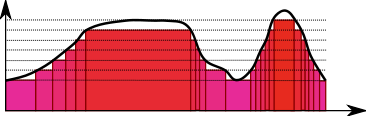
\includegraphics[scale=0.5]{images/lebesgue-integral-simple-functions.png}
    \caption{Lebesgue integration.
      \url{https://commons.wikimedia.org/wiki/File:Lebesgueintegralsimplefunctions.svg}}
    \label{fig:lebesgue-integration}
  \end{figure}
\end{proof}
\begin{prop}
  Parts a,b, and c from \ref{integration-props} apply to the new
  definition of integration for $f,g \in L^+$.
\end{prop}
\begin{proof}
  \begin{enumerate}
  \item[(a)] If $c=0$, the statement is trivial. Let $c > 0$. Then, \[
      \int c f \d\mu = \sup_{\phi \leq cf, \phi \text{ simple}} \int
      \phi \d\mu
    \]
    Take $\psi := \frac{1}{c}\phi$ is simple. Then, $\psi \leq f$
    and \[
      \int f \geq \int \psi = \int \frac{1}{c} \phi = \frac{1}{c} \int \phi
    \]
    which then implies that \[
      \int \phi \leq c \int f
    \]
    Then just take the supremum over $\phi$ to get \[
      \int cf \leq c \int f.
    \]
    Changing $c \to \frac{1}{c}$ yields the other inequality.
  \item[(c)] If $\phi$ is finite, we have $\phi \leq f \leq g$ and so
    $\int \phi \leq \int g$ by definition. Take supremum over $\phi$
    to get $\int f \leq \int g$.
  \item[(b)] If $0 \leq \phi \leq f$ and $0 \leq \psi \leq g$ for
    simple $\phi,\psi$, then $0 \leq \phi+\psi \leq f+g$ and so \[
      \int \phi + \int \psi = \int(\phi + \psi) \leq \int (f+g)
    \]
    by definition. Now, fix $\phi$ and take supremum over $\psi$ to
    get, for all $\phi$, that \[
      \int \phi + \int g \leq \int(f+g)
    \]
    and then take sup over $\phi$ to get \[
      \int f + \int g \leq \int(f+g).
    \]
    For the other inequality, we will need the following lemma
    \subsection*{(3/21/2017) Lecture 12}
    \begin{lem}\label{lem26}
  Let $f \in L^+$. Then, if $\phi_n$ is a sequence of simple functions
  with, for all $x$, $\phi_n(x)$ a non-decreasing sequence and
  $\lim_{n \to \infty} \phi_n(x) = f(x)$, then \[
    \lim_{n \to \infty} \int \phi_n \d\mu = \int f \d\mu
  \]
  \end{lem}
  Then, take $\phi_n$ a non-decreasing sequence converging to $f$ and
  $\psi_n$ a non-decreasing sequence converging to $g$. Then, $\phi_n
  + \psi_n$ simple functions converge to $f+g$ and so we apply the
  lemma to get
  \begin{align*}
    \int (f+g) \d\mu & = \lim_{n \to \infty} \int (\phi_n+\psi_n) \\
                    & = \lim_{n \to \infty}\left( \int \phi_n + \int \psi_n \right)\\
    & = \lim_{n \to \infty} \int \phi_n + \lim_{n \to \infty} \int
      \psi_n \\
    & = \int f + \int g
  \end{align*}
  \end{enumerate}
\end{proof}
Of course, we need to prove this lemma, so we seek to do that now.
\begin{prop}
  Let $\phi$ be simple in $L^+$. Then,
  \begin{enumerate}
  \item \[
      \nu_\phi(E) = \int_E \phi \d\mu := \int_X \phi \chi_E \d\mu
    \]
    is a measure.
  \item For all $\psi$ simple in $L^+$, \[
      \int \psi d\nu_\phi = \int \psi \phi d \mu
    \]
  \end{enumerate}
  \begin{proof}
    (a) is trivial. For (b), we must call Bootstrap Bill.
    \begin{itemize}
    \item ($\psi = \chi_E$). If $\psi = \chi_E$, then $\psi = 1 \cdot
      \chi_E + 0 \cdot \chi_{E^c}$ is a good decomposition of
      $\psi$. Thus, \[
        \int \psi d\nu_\phi = \nu_\phi(E) = \int \chi_E \phi d \mu =
        \int \psi \phi \d\mu
      \]
    \item (General $\psi$). Let $\psi$ have a good decomposition $\psi
      = \sum_{i=1}^n a_i \chi_{E_i}$ for $a_i \in [0,\infty)$ and
      $\Dunion E_i = X$. By definition, we get that
      \begin{align*}
        \int \psi d\nu_\phi & = \sum_{i=1}^n a_i \int \chi_{E_i} d
                         \nu_\phi \\
                       & = \sum a_i \int \chi_{E_i} \phi \d\mu \\
                       & = \int \left( \sum a_i \chi_{E_i} \right)
                         \phi \d\mu \\
        & = \int \psi \phi \d\mu
      \end{align*}
    \end{itemize}
  \end{proof}
\end{prop}
\begin{prop}
  Let \((\phi_n)_{n \geq 1}, \psi\) all be simple functions such that
  \(\phi_n\) increases to \(\psi\). Then, \[
    \lim_{n \to \infty} \int \phi_n \d\mu = \int \psi \d\mu
  \]
\end{prop}
\begin{proof}
  Let \(\alpha \in [0,1) \) and, for all \(n\), let \(E_n = \{x
  \in X \st \phi_n(x) \geq \alpha \psi(x)\}\). It is clear that
  \(E_n\) is measurable since \(\phi_n - \alpha \psi\) is measurable
  and \(E_n\) is the inverse image of \([0,\infty) \). Furthermore, it
  is easy to check \(E_n \subset E_{n+1}\). Now, we note that \[
    \Union_{n=1}^\infty E_n = X.
  \]
  Let \(x \in X\). If \(\psi(x) = 0\), then \(x \in E_n\). Otherwise,
  \(\psi(x) > 0\) is finite and so \(\alpha \psi(x) < \psi(x)\). Thus,
  \(\phi_n(x) \to \psi(x)\) and thus there exists an \(n\) such that
  \(\phi_n(x) \geq \alpha \psi(x)\). Thus, we now have \[
    \lim \int \phi_n \leq \int \psi.
  \]
  We still want to show the other inequality. Consider \(\nu_{\alpha
    \psi}\). We have that \(\nu_{\alpha \psi}(E_n) \to \nu_{\alpha
    \psi}(X)\) as \(n \to \infty \) using continuity from
  below. Furthermore, \[
    \nu_{\alpha \psi}(X) = \int \chi_X \alpha \psi \d\mu = \alpha \int
    \psi \d\mu.
  \]
  Now, \(\phi_n \geq \alpha \psi \chi_{E_n}\) for all \(x \in X\) and
  thus \[
    \int \phi_n \d\mu \geq \int \alpha \psi \chi_{E_n} \d\mu = \nu_{\alpha \psi}(E_n).
  \]
  Taking \(n \to \infty\), we get \[
    \lim \int \phi_n \d\mu \geq \alpha \int \psi \d\mu
  \]
  for \(\alpha \in (0,1)\) and so we take \(\alpha \to 1\) to complete
  the proof.
\end{proof}
Finally, we can now prove \ref{lem26}.
\begin{proof}[Proof of Lemma]
  Take \((\phi_n)\) as a sequence of simple functions increasing to
  \(f\) in \(L^+\). Since \(0 \leq \phi_n \leq f\), we get \[
    \int \phi_n \leq \int f
  \]
  by definition and so \[
    \lim_{n \to \infty} \int \phi_n \leq \int f.
  \]
  To get the \(\geq\) direction, take \(0 \leq \phi_n \leq f\). Also,
  let \(\psi\) be any simple function with \(\phi_n \leq \psi\). Then,
  \(\min(\phi_n,\psi)\) is simple and increases to \(\psi\). Thus, by
  our proposition above, we get that \[
    \lim \int \phi_n \geq \lim \int \min(\phi_n,\psi) = \int \psi
  \]
  However, this is true for all \(\psi \leq f\). So, taking the supremum, we
  get \[
  \lim_{n \to \infty} \int \phi_n \geq \int f.
  \]
\end{proof}
\begin{thm}[Monotone Convergence theorem]
  Let \((f_n)_{n \geq 1}, f \in L^+\) with \(f_n\) increasing to
  \(f\). Then, \[
    \lim_{n \to \infty} \int f_n \d\mu = \int f \d\mu
  \]
\end{thm}
\begin{proof}
  The \(\leq\) direction is trivial by properties of integrals. For
  the \(\geq\) direction, let \(\alpha \in (0,1)\) and \(\psi\) be
  a simple function with \(0 \leq \psi \leq f\). Furthermore, let
  \(E_n = \{x \in E \st f_n(x) \geq \alpha \psi(x)\}\), which is
  measurable as discussed in the previous proof of the proposition, as
  well as increasing and satisfying \(\Union_n E_n = X\). Now,
  consider \(\nu_{\alpha \psi}\) as a measure. We have that
  \(\nu_{\alpha \psi}(E_n) \to \nu_{\alpha \psi}(X)\) and so this
  gives us that \[
    \int f_n \d\mu \geq \int \alpha \psi \chi_{E_n} \d\mu \to \alpha
    \int \psi \implies \lim_{n \to \infty} \int f_n \d\mu \geq \alpha
    \int \psi \d\mu
  \]
  Since this is true for all \(\alpha \in (0,1)\), it is true for
  \(\alpha = 1\). Now, simply take the supremum over \(\psi\) to get
  the theorem.
\end{proof}
Here I will choose to judiciously skip some pages of notes for the
sake of getting the more important theorems into the notes.
\begin{lem}[Fatou's Lemma]
  Let \((f_n)_{n \geq 1} \in L^+\). Then, \[
    \int (\lim \inf f_n) \d\mu \leq \lim \inf \int f_n \d\mu
  \]
\end{lem}
\begin{proof}
  For a perfectly good proof using our program, see page 52 of
  Folland, 2.18.
\end{proof}
\subsection*{(3/23/2017) Lecture 13}
\begin{prop}
  Let \((X,\M,\mu)\) be a measure space with \(f \in L^+\). If
  \(\mu(E) = 0\), then \(\nu_f(E) = 0\).
\end{prop}
\begin{defn}
  Let \((X,\M)\) be a measurable space with measures \(\mu,\nu\) both
  defined on it.
  \begin{enumerate}
  \item \(\nu\) is called \de{absolutely continuous with respect to
      \(\mu\)} (denoted \(\nu \ll \mu\)) if and only if for all \(E
    \in \M\), \(\mu(E) = 0 \implies \nu(E) = 0\).
  \item \(\mu\) is \de{singular with respect to \(\nu\)} if and only
    if there exists an \(E \in \M\) such that \(\nu(E) = \mu(E^c) =
    0\).
  \end{enumerate}
\end{defn}
\begin{prop}
  \(\mu\) is singular with respect to \(\nu\) if and only if \(\nu\)
  is singular with respect to \(\mu\).
\end{prop}
\begin{defn}
  \(\mu\) and \(\nu\) in the proposition above may be called
  \de{mutually singular}, denoted \(\mu \perp \nu\).
\end{defn}
\begin{rmk}
  If \(\nu \ll \mu\) and \(\nu \perp \mu\), then \(\nu \equiv 0\).
\end{rmk}
\begin{rmk}
  For all \(f \in L^+\), \(\nu_f \ll \mu\). Later, we will see the
  converse in the Radon-Nicodyn Theorem.
\end{rmk}
I am choosing to skip the section of restriction of measures to
subsets.
\begin{defn}
  We say measurable \(f \from X \to \R\) is \de{integrable} if and only if \[
    \int |f| \d\mu < \infty.
  \]
  We denote this \(f \in \cL^1(X,\R) = \cL^1(X,\M,\mu,\R)\)
\end{defn}
\begin{defn}
  Let \(f \in \cL^1\). A \de{good representation} of \(f\) is \[
    f = g-h
  \]
  where \(g,h \in \cL^1\) take values in \([0,\infty]\) and are
  measurable.
\end{defn}
\begin{defn}
  \[
    \int_X f \d\mu := \int_X g \d\mu - \int_X h \d\mu
  \]
\end{defn}
We would need to show this definition makes sense. Once again, I will
omit such details for the time being.
\begin{prop}
  Let \(\mathbb{K} = \R,\C\), or \([0,\infty]\). Then,
  \begin{enumerate}
  \item \(\cL^1(X,\mathbb{K})\) is a \(\mathbb{K}\)-vector space.
  \item \(f \mapsto \int_X f \d\mu\) is a \(\mathbb{K}\)-linear form.
  \end{enumerate}
\end{prop}
\subsection*{(3/23/2017) Lecture 14}
\begin{prop}
  Let \(\mathbb{K} = \R,\C\) and \(f \in
  \cL^1(X,\mathbb{K})\). Then, \[
    \left| \int f \right| \leq \int \left| f \right|
  \]
\end{prop}
\begin{prop}
  Using the same hypotheses as above,
  \begin{enumerate}
  \item \(f \in \cL^1 \implies \{x \st f(x) \neq 0\}\) is
    \(\sigma\)-finite.
  \item For all \(f,g \in \cL^1\), \[
      \int_E f = \int_E g, \ \forall E \in \M \iff \int |f-g| = 0 \iff
      f=g \ \mu-\text{almost everywhere}.
    \]
  \end{enumerate}

\end{prop}
\begin{defn}
  \(L^1 = \cL^1/\sim\) where \(f \sim g\) if \(f=g\) \(\mu\)-almost everywhere.
\end{defn}
\section{Elements of Functional Analysis}
\subsection{Topological Vector Spaces}
\begin{defn}
  Let \(V\) be a \(\mathbb{K} = \R,\C\) vector space. \(V\) is called
  a \de{\(\mathbb{K}\)-topological vector space} (TVS) if \(V\) comes with
  a topology \(\Top\) such that \(+ \from V \times V \to V\) and
  \(\cdot \from \mathbb{K} \times V \to V\) are continuous.
\end{defn}
\begin{defn}
  Give \(V\) a \(\mathbb{K}\)-vector space, \(||\cdot|| \from V \to
  [0,\infty)\) is called a \de{semi-norm} if
  \begin{enumerate}
  \item for all \(u,v \in V\), \(||u+v|| \leq ||u|| + ||v||\)
  \item for all \(\lambda \in \mathbb{K}\) and \(v \in V\),
    \(||\lambda v|| = |\lambda|\cdot ||V||\)
  \end{enumerate}
\end{defn}
Note that this differs from the definition of a norm since \(||v||=0\)
does not imply \(v = 0\).
\begin{defn}
  \(||\cdot||\) is a \de{norm} if it is a seminorm with the property
  \(||u||=0\) if and only if \(u = 0\).
\end{defn}
\begin{defn}
  Given a finite set of semi-norms \(F\) on a vector space \(V\),
  define a \de{multi-ball} with radius \(\epsilon > 0\) to be \[
    B(u,F,\epsilon) = \left\{ v \st \ \forall ||\cdot|| \in F, ||v-u|| <
    \epsilon\right\}
  \]
\end{defn}
\begin{defn}
  Let \(V\) be a \(\mathbb{K}\)-vector space and let \(\cN\) be a set
  of semi-norms \(\cN \subset [0,\infty)^V \). Then, there is a
  canonical topology \(\Top_\cN\) on \(V\) which makes it a
  topological vector space. Namely, \[
    \Top_\cN = \left\{ U \in \P(V) \st \forall u \in U, \exists \text{
      finite } F \subset \cN, \exists \epsilon > 0,
  B(u,F,\epsilon) \subset U \right\}
  \]
\end{defn}
\subsection*{(3/28/2017) Lecture 15}
\begin{defn}
  Let \(V\) be a TVS with topology \(\Top_\norms\) for some set of
  semi-norms \(\norms\). Then, we call \((V,\Top_\norms)\) a
  \de{locally convex topological vector space} (LCTVS).
\end{defn}
\begin{rmk}
  \(B(x,F,\epsilon)\) with finite \(F \subset \norms\), \(x \in
  V\), and \(\epsilon > 0\) is an open set in \(\Top_\N\).
\end{rmk}
\begin{proof}[Proof of remark]
  Let \(F = \{\norm_1, \ldots, \norm_k\}\). Then, take \(y \in
  B(x,F,\epsilon)\). We want to find some \(\epsilon' > 0\) such that
  \(B(y,F,\epsilon') \subset B(x,F,\epsilon)\). Now, if we take \(1
  \leq \ell \leq k\), we get \[
    \norm[x-z]_\ell \leq \norm[x-y]_\ell + \norm[y-x]_\ell <
    \norm[x-y]_\ell + \epsilon'
  \]
  and we want this to be less than \(\epsilon\), so take \(\epsilon' =
  \min_{1 \leq \ell \leq k}(\epsilon - \norm[x-y]_\ell)\).
\end{proof}
\begin{prop}
  Given \(V,\Top_\norms\) an LCTVS, it is Hausdorff separated if and
  only if, for all \(x \in V \setminus \{0\}\) there exists \(\norm
  \in \norms\) with \(\norm[x] \neq 0\).
\end{prop}
\begin{proof}
  \begin{itemize}
  \item (\(\implies\)). Take \(x \neq 0\) and \((V,\Top_\norms)\)
    Hausdorff separated. Then, there are \(U_1,U_2\) open disjoint
    sets with \(0 \in U_1\) and \(x \in U_2\). Therefore, there exists
    \(F,\epsilon\) such that \(0 \in B(0,F,\epsilon) \subset U_1\) but
    \(x\) is not. Thus, there exists an \(\ell, 1 \leq \ell \leq k\)
    such that \(\norm[x]_\ell \geq \epsilon > 0\).
  \item (\(\impliedby\)). Let \(x,y \in V\)with \(x \neq y\). Then
    there exists \(\norm\) such that \(\epsilon := \norm[x-y] >
    0\). Thus, take \(F = \{\norm\}\) and we get that \[
      B\left(x,F,\frac{\epsilon}{2}\right) \intersect B\left(y,F,\frac{\epsilon}{2}\right) = \emptyset
    \]
  \end{itemize}
\end{proof}
We will mostly focus on Hausdorff LCTVS's.
\begin{defn}
  \(X,\Top\) a topology is called \de{first countable} if, for all
  \(x\), there exists a sequence \((V_n)_{n \geq 1}\) of open
  neighborhoods of \(x\) such that, for all \(U \in \Top\) with \(x
  \in U\), there exists an \(n\) with \(V_n \subset U\).
\end{defn}
Without loss of generality, we can assume \((V_n)\) is decreasing
using the standard trick.
\begin{example}
  All metric spaces \(X,d\) are first countable by taking \(V_n =
  B(x,\frac{1}{n})\).
\end{example}
\begin{prop}[Sequential Characterization of Limits]\label{seq-char-of-lims}
  Suppose \(X, \Top_X\) is first countable with \(\Top_\infty \subset
  X\) a union of neighborhoods of a point \(x_\infty \in X\). Then,
  given a function \(f \from U \setminus \{x_\infty\} \to (Y,
  \Top_Y)\) and \(y \in Y\), we have \(\lim_{x \to x_\infty} f(x) = y\)
  if and only if, for all sequences \((x_n)\) in \(U \setminus
  \{x_\infty\}\) such that \(x_n \to x_\infty\), we get \(f(x_n) \to y\).
\end{prop}
\begin{proof}
  \begin{itemize}
  \item (\(\implies\)). Take \(W \in \Top_Y, y \in W\) with \(\lim_{x
      \to x_\infty} f(x) = y\). Thus, there exists a \(V \in \Top_X,
    x_\infty \in V, V \subset U\) such that for all \(x \in V
    \setminus \{x_\infty\}\), \(f(x) \in W\). Thus, \(\lim f(x_n) =
    y\).
  \item (\(\impliedby\)). We seek to prove the contrapositive. Let
    there exist a \(W\) open neighborhood of \(y\) such that, for all
    \(V \in \Top_X\) with \(x_\infty \in V\) and \(V \subset U\),
    there exists \(x \in V \setminus \{x_\infty\}\) such that \(f(x)
    \not \in W\). Here we use the first countable property, so there
    exists a non-increasing \((V_n)\) that is a neighborhood basis for
    \(x_\infty\). Without loss of generality \((V_n) \subset
    U\). Thus, there exists an \(N\) such that, for all \(n \geq N\),
    \(V_n \subset U\). So, we renumber our sequence from \(N\) and
    apply above to \(V = V_n\) to get that there exists an \(x_n \in
    V_n \setminus \{x_\infty\}\) with \(f(x_n) \not \in W\). Thus,
    \(\lim_{n \to \infty} f(x_n) = y\) is false. Moreover, \(x_n \neq
    x_\infty\) for all \(n\), but \(\lim x_n = x_\infty\). If
    \(\Omega\) is a neighborhood of \(x_\infty\), there exists an
    \(n\) where \(V_n \subset \Omega\) implies that, for all \(m \geq
    n\), \(V_m \subset \Omega\).
  \end{itemize}
\end{proof}
\begin{prop}
  Let (\(V,\Top_\norms\)) be a Hausdorff LCTVS. Then, the following
  are equivalent.
  \begin{enumerate}
  \item \(V\) is metrizable.
  \item \(V\) is first countable.
  \item There exists a countable \(\norms_c \subset \norms\) such that
  \(\Top_{\norms_c} = \Top_\norms\).
  \end{enumerate}
\end{prop}
\begin{proof}
  (a) implies (b) is trivial since all metric spaces are first
  countable. The proofs of the other two statements are omitted for
  the time being since they are somewhat long and technical.
\end{proof}
\begin{rmk}
  In summary, we have that, given a Hausdorff LCTVS
  \((V,\Top_\norms)\) (where \(\norms\) is non-unique), we ask what is
  the smallest \(\norms\) needed to define our topology?
  \begin{itemize}
  \item If \(\norms\) is finite, we have shown we really only need one
    norm.
  \item If \(\norms\) is countable, we have shown \(V\) is metrizable.
  \item If \(\norms\) is uncountable, then \(V\) is not metrizable
    (see homework 6).
  \end{itemize}
\end{rmk}
\begin{example}
  The space of all functions \(f \from \R^d \to \mathbb{K}\) that are
  in \(\mathcal{C}^\infty\)
\end{example}
We now seek to fix some notation.
\begin{defn}
  \begin{itemize}
  \item Take \(\alpha \in \N_0^d\) as a multi-index. \(\alpha =
    (\alpha_1, \ldots, \alpha_d)\).
  \item Say \(|\alpha| = \alpha_1 + \cdots + \alpha_d\) the \de{length
      of \(\alpha\)}.
  \item \[
      \partial^\alpha f(x) := \frac{\partial^{|\alpha|}}{\partial
        x_1^{\alpha_1} \cdots \partial x_d^{\alpha_d}}(x)
    \]
  \item \(\langle x \rangle := \sqrt{1+\norm[x]_2^2}\) where
    \(\norm_2\) is the standard Euclidean norm.
  \item For all \(\alpha\) and \(k \geq 0\), \[
      \norm[f]_{\alpha,k} := \sup_{x \in \R^d} \langle x \rangle^k
      \left| \partial^d f(x) \right| \in [0,\infty]
    \]
  \item Define the \(\mathbb{K}\)-vector space \[
      S(\R^d,\mathbb{K}) := \left\{ f \from \R^d \to \mathbb{K} \in
        \mathcal{C}^\infty \st \forall \alpha, k, \norm[f]_{\alpha,k}
        < \infty \right\}
    \]
  \item Thus, \(\norm_{\alpha,k}\) restricted to \(S\) are seminorms
    on \(S\), so we say \[
      \norms = \{\norm_{\alpha,k} \st \alpha \in \N_0^d, k \in \N_0\}.
    \]
  \end{itemize}
  So, \(S(\R^d,\mathbb{K}), \Top_\norms\) is a \(\mathbb{K}\)-LCTVS
  metrizable space called \de{Schwartz space}. Also, let
  \(S'(\R^d,\mathbb{K})\) be its topological dual, that is, continuous
  \(\mathbb{K}\)-linear forms \(S \to K\).
\end{defn}
\subsection*{(3/30/2017) Lecture 16}
Take \(d=1\), then we can study \(L^1(\R,m,\K) \to S'(\R,\K)\) given
by \(f \mapsto L_f\), a linear form on \(S\). So, \(L_f(g) = \int_\R
fg \d m\) for \(g \in S\). However, we would like to pick \(f \in
\cL^1\) a representative and show that this form is well-defined, linear,
and continuous in both variables.
\begin{prop}[\(L^1-L^\infty\) bound]\label{L1-Linf-bound-1}
  Given \(f,g\) measurable functions with \(f \in L^1\) and \(g\)
  continuous and bounded, we get \[
    \int |fg| \d m \leq \norm[f]_{L^1} \cdot \norm[g]_\infty =
    \left(\int_\R |f| \d m\right) \cdot \sup_{x \in \R} |g(x)|.
  \]
\end{prop}
...
\begin{rmk}
  We will skip sections 3.1 and 3.3 in Folland on signed measures and
  complex measures respectively.
\end{rmk}
\begin{defn}
  We say \(f \from X \to Z\) is \de{locally constant} if, for all \(x \in
  X\), there exists an open set \(U \subset X\) with \(x \in U\) such
  that, for all \(y \in U\), we get \(f(y) = f(x)\).
\end{defn}
Note that a locally constant function is continuous.
\begin{defn}
  Let \(f \from X \to \K\). We define the \de{support of \(f\)} to
  be \[
    \supp(f) = \ov{\{x \st f(x) \neq 0\}}
  \]
\end{defn}
\begin{defn}
  Let \(f \from X \to \K\). We say \(f\) is \de{compactly supported}
  if \(\supp(f)\) is compact.
\end{defn}
We now take some time to do an aside on \(p\)-adic numbers, which one
should recall from homeworks 1 and 4.
\begin{defn}
  Recall that the \(p\)-adic numbers, \(\Q_p\), are the normed vector
  space with elements \[
    x = \sum_{n \in \Z} a_n(x) p^n, \ a_n(x) \in \{0, \ldots, p-1\}
  \]
  such that \(a_n(x) = 0\) for negative enough \(n\), and norm \[
    |x|_p = p^{-k}
  \]
  where \(k \in \Z\) is the index such that \(a_k(x) \neq 0\), but
  \(a_n(x) = 0\) for all \(n < k\). Note that this also gives the nice
  characterization that \[
    |x-y|_p = p^{-N} \text{ where } N = \min\{n \st a_n(x) \neq a_n(y)\}.
  \]
  is a metric and so we can define closed balls \(B(x,p^k)\) for \(k
  \in \Z\).
\end{defn}
\begin{rmk}
  Taking \(d \from \Q_p \times \Q_p \to [0,\infty)\) as \(d(x,y) :=
  |x-y|_p\), we have that \(d\) is actually an \de{ultrametric}, that
  is \[
    d(x,z) \leq \max(d(x,y), d(y,z))
  \]
\end{rmk}
\begin{defn}
  Given \(d \in \N\), we define the \de{Schwartz-Bruhat} space as \[
    S(\Q_p^d,\K) := \left\{ f \from \Q_p^d \to \K \st f \text{ is
        locally constant and compactly supported} \right\}.
  \]
  It is easy to show this is a \(\K\)-vector space.
\end{defn}
\begin{example}
  If we take \(\norms_\text{all}\) to be the set of all seminorms on
  \(S(\Q_p^d,\K)\) and equip it with the topology
  \(\Top_{\norms_\text{all}}\), then we get \(S'(\Q_p^d,\K)\) as the
  topological dual of \(S\). In this case, it also happens to coincide
  with the algebraic dual.
\end{example}
\begin{prop}
  Let \(f \in S(\Q_p,\K)\). Then, there exists \(k,\ell \in \Z\) with
  \(k \leq \ell\) such that
  \begin{enumerate}
  \item \(\supp(f) \subset B(0,p^\ell)\)
  \item For all \(x,y \in \Q_p\), \(|x-y|_p \leq p^k \iff f(x) =
    f(y)\).
  \end{enumerate}
\end{prop}
\begin{proof}[``Proof'']
  For some \(ell\), we have \(\supp(f) \subset B(0,p^\ell)\) and a
  locally constant function on a compact metric space gives us a
  uniform local constant.
\end{proof}
\begin{defn}
  Let \(k,\ell \in \Z\) with \(k \leq \ell\). Define
  \(S_{k,\ell}(\Q_p,\K) = \{f \st \text{ (a) and (b) from the
    proposition above hold}\}\). So, \[
    S(\Q_p,\K) = \Union_{k,\ell} S_{k,\ell} = \Union_{n \in \N} S_{-n,n}
  \]
\end{defn}
We note that \(\dim_\K S_{k,\ell}\) is the number of closed balls of
radius \(p^k\) inside \(\ov{B}(0,p^\ell)\), which is \(p^{\ell-k}\).
\begin{rmk}
  We get that \(S = \Union_{n \geq 0} S_{-n,n} \isom \bigoplus_{n \in
    \N_0} \K = \K[x] \) and so there exists a countable Hamel basis
  for \(S\).
\end{rmk}
\subsection*{(3/30/2017) Lecture 17}
\begin{defn}
  Given a LCTVS \((V,\Top_\norms)\), define \[
    V_{\text{null}} := \left\{ x \in V \st \forall \norm \in \norms,
      \norm[x] = 0 \right\}.
  \]
  This is a \(\mathbb{K}\)-linear subspace of \(V\).
\end{defn}
\begin{rmk}
  Given LCTVS \((V,\Top_\norms)\)  that is not Hausdorff, one can fix
  this by defining the equivalence relation \(x \sim y \iff \forall
  \norm, \norm[x-y] = 0\). Then \(\ov{V} := V/\sim\) is
  Hausdorff. Equivalently, one could define \(\ov{V} :=
  V/V_{\text{null}}\). We then get \(\ov{\norms}\) on \(\ov{V}\) given
  by \(\{\ov{\norm} \st \norm \in \norms\}\) where \(\ov{\norm[[x]]}
  := \norm[x]\), which is clearly well-defined. Thus, \(\ov{\norm}\)
  is a seminorm of the quotient \(\ov{V}\) and so we get an LCTVS
  \((\ov{V}, \Top_{\ov{\norms}})\).
\end{rmk}
\begin{example}
  Take \(V = \cL^1(X,\M,\mu,\mathbb{K})\), \(\norms =
  \{\norm_{L^1}\}\), \(\norm[f]_{L^1} = \int_X |f|\d\mu\), \(\ov{V} =
  L^1(X,\M,\mu,\mathbb{K})\), and \(V_\text{null} = \{f \st f=0
  \mu-\text{almost everywhere}\}\).
\end{example}
\subsection{Normed spaces}
\begin{defn}
  Given a space \(V\) and a norm \(\norm\),  \((V,\norm)\) is called a
  \de{normed space} if it is equipped with the metric topology using
  the metric \(d(x,y) = \norm[x-y]\).
\end{defn}
\begin{defn}
  A normed space \((V,\norm)\) is a \de{Banach space} if it is
  complete.
\end{defn}
We will eventually show that \(L^1(X,\M,\mu,\mathbb{K})\) is a Banach
space.
\begin{rmk}
  Given \(f \in L^1\), \(\int_X f \d\mu\) is well-defined independent
  of choice of representative.
\end{rmk}
\begin{thm}[Dominated Convergence Theorem v1.0]\label{dct-v1}
  Let \((X,\M,\mu)\) be a measure space and let \(f_n \from X \to
  \mathbb{K}\) be a sequence of functions in \(\cL^1\) such that, for
  all \(x\), \(\lim_{n \to \infty} f_n(x)\) exists and there exists an
  integrable \(g \in L^+ \intersect \cL^1\) with \(\infty > g \geq
  0\) such that, for all \(n \geq 1\) and for all \(x\), \(|f_n(x)|
  \leq g(x)\) (that is to say, \(g\) is a dominating function), then
  \(f \in \cL^1\) and \[
    \lim_{n \to \infty} \int_X f_n \d\mu = \int_X f \d\mu
  \]
\end{thm}
\begin{proof}
  We first note that if \(f\) is the pointwise limit of measurable
  functions, then \(f\) is measurable. Thus, \(\norm[f_n(x)] \leq
  g(x)\) for all \(n\) tells us \(\norm[f(x)] \leq g(x)\) in
  \(\cL^1\). Thus, since \(g \in \cL^1\), \[
    \int g < \infty \implies \int |f| < \infty
  \]
  and so \(f \in \cL^1\).
  \begin{itemize}
  \item (\(\K = \R\)). Let \(f_n(x) + g(x) \geq 0\) for all
    \(x,n\). Then we use Fatou's lemma.
    \begin{align*}
      \int \lim \inf (f_n+g)
      & \leq \lim \inf \int (f_n+g) \text{ in }L^+ \\
      & \leq \lim \inf \int (f_n+g) \text{ in }\R \\
      \implies \int f + \int g & \leq \left( \lim \inf \int f_n \right)
      + \int g \\
      \implies \int f \leq \lim \inf \int f_n & \leq \lim \sup \int f_n
    \end{align*}
    Now, we wish to show \(\lim \sup \int f_n \leq \int f\). Take
    \(-f_n(x) + g(x) \geq 0\) and do the argument above again for
    \(-f_n\). This will yield \[
      \int (-f) \leq \lim \inf \int (-f_n)
    \]
    and so moving the minus signs outside gets \[
      \int f \geq \lim \sup \int f_n
    \]
    and so we are done.
  \item (\(\K = \C\)). Simply use the real case on \(|\operatorname{Re}
   f_n| \leq |f_n| \leq g\) and similarly for the imaginary part.
  \end{itemize}
\end{proof}
\begin{thm}[Dominated Convergence Theorem v2.0, ``\(\mu\)-almost
  everywhere everywhere'']
  Let \((f_n)\) be integrable and \(g \geq 0\) be
  integrable. Furthermore, for all \(n\), let \(|f_n| \leq g\)
  \(\mu\)-almost everywhere and let \(\lim_{n \to \infty} f_n(x)\)
  exist \(\mu\)-almost everywhere. Then, ``\(f \in L^1\)''  and \(\lim_{n
    \to \infty} \int f_n = \int f\).
\end{thm}
\begin{rmk}
  ``\(f \in L^1\)'' means there exists a true function \(f \in \cL^1\)
  such that, for \(\mu\)-almost all \(x\), \(\lim_{n \to \infty}
  f_n(x) = f(x)\) exists. If \(g \in \cL^1\), it also works with
  \(f=g\) \(\mu\)-almost everywhere.
\end{rmk}
\begin{proof}
  There exists \(Z,(Z_n)_{n \geq 1}\) in \(\M\) of measure 0 such that
  \(|f_n(x)| \leq g(x)\) on \(Z_n^c\) and such that \(\lim_{n \to
    \infty} f_n(x)\) exists on \(Z^c\). Take \(N = Z \union \left(
    \Union_{n \geq 1} Z_n \right)\). Then, we let \[
    f(x) :=
    \begin{cases}
      \lim_{n \to \infty} f_n(x) & \text{ if } x \in N^c \subset Z^c
      \\
      0 & \text{ else }
    \end{cases}
  \]
  Then, we have that \(f_n \chi_{N^c} \to f\) pointwise everywhere
  and, for all \(n\), \(|f_n \chi_{N^c}| \leq g\). Thus, we can use
  the Dominated Convergence Theorem 1.0 to conclude that \(f \in
  \cL^1\) and, moreover, that \(\lim \int f_n \chi_{N^c} = \int f\).
\end{proof}
\subsection*{(4/4/2017) Lecture 18}
\begin{example}
  Take \((\N,\B_\N,\mu)\) as a measure space where \(\mu\) is the
  counting measure. Then, a function \(f \from \N \to \K\) is a
  sequence \(a = (a_n)_{n \geq 1}\). If \(a \in L^1\), then \[
    \int_\N |a_n| \d\mu(w) = \sum_{n=1}^\infty |a_n| < \infty
  \]
  and thus saying \(a \in L^1(\N,\K)\) is the same as saying the
  series corresponding to \(a\) converges absolutely.
\end{example}
\begin{defn}
  We defined \(\ell^1 = \ell^1(\N,\K) := L^1(\N,\P(\N),\mu,\K)\) where
  \(\mu\) is the counting measure. This is a normed space with \[
    \norm[a]_{L^1} = \sum_{n=1}^\infty |a_n|
  \]
\end{defn}
\begin{cor}
  Let \((a_{i,j})_{(i,j) \in \N^2}\) with values in \(\C\) such that
  there exists a sequence
  \((b_i)_{i \geq 1}\) with \(\sum_{i=1}^\infty a_{i,j} <
  \sum_{i=1}^\infty b_i < \infty\).
  Then, \[
    \sum_{i=1}^\infty \lim_{j \to \infty} a_{i,j}
  \]
  is absolutely convergent and we get the equality \[
    \sum_{i=1}^\infty \lim_{j \to \infty} a_{i,j} = \lim_{j \to
      \infty} \sum_{i=1}^\infty a_{i,j}
  \]
\end{cor}
\begin{proof}
  Proof is elementary and left as exercise.
\end{proof}
\begin{thm}[Dominated Convergence Theorem v2.1, Series Version]
  Let \((f_n)_{n \geq 1}\) be a sequence in \(L^1\) such that
  \(\sum_{n=1}^\infty \norm[f_n]_{L^1} < \infty\). Then, \(\lim_{N \to
  \infty} \sum_{n=1}^N f_n =: f\) exists
  and \[
    \sum_{n=1}^\infty \int_X f_n \d\mu = \int_X f \d\mu
  \]
\end{thm}
\begin{proof}
  The proof is a combination of using MCT and DCT. Take representatives
  in \(\cL^1\) for \(f_n\) and define \[
    g(x) := \sum_{n=1}^\infty |f_n(x)|.
  \]
  (Read ahead to see why this converges.) Then, using a MCT corollary, we
  get \[
    \int g \d\mu = \sum_{n=1}^\infty \int |f_n| \d\mu < \infty.
  \]
  Thus, it must be that \(g(x) < \infty\) \(\mu\)-almost everywhere.
  Thus, one construction we could use is, given \(Z \in \M\) the set
  of measure 0 on which \(g(x) = \infty\), we can define \[
    \tilde{g}(x) =
    \begin{cases}
      g(x) & \text{ if } x \not\in Z \\
      0 & \text{ else }
    \end{cases}
  \]
  So, \(\tilde{g} \in \cL^1\) and \(L^1\) with \(\tilde{g}(x) <
  \infty\) for all \(x\). Now, to use DCT v2.0, we note \[
    \left| \sum_{n=1}^N f_n(x) \leq \tilde{g}(x) \right|, \
    \mu\text{-almost everywhere}
  \]
  and so \[
    \lim_{N \to \infty} \int \sum_{n=1}^N f_n(x) = \int f(x) dx.
  \]
  Finally, we check that \[
    \norm[f - \sum_{n=1}^\infty f_n]_{L^1} = \int \left|
      \sum_{n=N+1}^\infty f_n \right| \leq \int \sum_{n=N+1}^\infty
    |f_n| = \sum_{n=N+1}^\infty \norm[f_n]_{L^1} \to 0 \text{ as } N
    \to \infty
  \]
  where the last equality follows from MCT.
\end{proof}
\subsection{Aside: \(\K\)-valued measures}
\begin{defn}
  Given a measurable space \((X,\M)\), a \(\K\)-valued measure is a
  function \(\mu \from \M \to \K\) such that \(\mu(\emptyset) = 0\)
  and if \(E = \Dunion_{n=1}^\infty E_n\), a disjoint union, then \[
    \sum_{n=1}^\infty \mu(E_n) = \mu(E) \text{ converges absolutely}
  \]
  is called a \de{signed measure} if \(\K=\R\) and a \de{complex
    measure} is \(\K=\C\).
\end{defn}
\begin{rmk}
  One can drop the absolute convergence from the definition, but then
  one needs the Riemann series rearrangement theorem.
\end{rmk}
\begin{prop}
  Let \(f \in \cL^1(X,\M,\mu,\K)\). Then, given \(E \in \M\), \[
    \nu_f(E) = \int_E f \d\mu := \int_X f \chi_E \d\mu
  \]
  is a \(\K\)-valued measure such that, for all \(E\), \(|\nu_f(E)|
  \leq \nu_{|f|}(E)\).
\end{prop}
Note that this agrees with the old definition.
\begin{proof}
  See Folland page 94, Proposition 3.13(a)
\end{proof}
\subsection{Restriction to Subsets}
In this section, we would like to introduce the idea of extension by
0.
\begin{prop}
  Let \((X,\M,\mu)\) be a measure space and let \(Y \in \M\). Then,
  using notation from before, we have \[
    \M_Y := \P(Y) \intersect \M, \ \mu_Y = \mu|_{\M_Y}.
  \]
  Let \(f \from Y \to \K\) be \((\M_Y,\B_\K)\)-measurable and let
  \(\tilde{f} \from X \to \K\) be its ``extension by zero'', that
  is \[
    \tilde{f} =
    \begin{cases}
      f(x) & \text{ if }x \in Y \\
      0 & \text{ else }
    \end{cases}
  \]
  Then, we have
  \begin{enumerate}
  \item \(\tilde{f}\) is \((\M,\B_\K)\)-measurable.
  \item \(f \in \cL^1(Y,\M_Y,\mu_Y,\K)\) if and only if \(\tilde{f}
    \in \cL^1(X,\M,\mu,\K)\), in which case \[
      \int_Y f \d\mu_Y = \int_X \tilde{f} \d\mu = \int_X \tilde{f}
      \chi_Y \d\mu = \int_Y \tilde{f} \d\mu = \int_Y f \d\mu
    \]
  \end{enumerate}
\end{prop}
\begin{proof}
  \begin{enumerate}
  \item Let \(B \in \B_\K\). Then, we get \[
      \tilde{f}^{-1}(B) = \left( \tilde{f}^{-1}(B) \intersect Y
      \right) \union \left( \tilde{f}^{-1}(B) \intersect Y^c \right)
    \]
    However, the left set is just \(f^{-1}(B) \in \M_Y \subset \M\)
    and the right set is either empty or equal to \(Y^c\), either of
    which is in \(\M\).
  \item We have the if and only if statement because \(|\tilde{f}| =
    \widetilde{|f|}\) using the previous version of this proposition
    (currently missing) for \(L^+\). Thus, we have \[
      \int_X |\tilde{f}| \d\mu = \int_Y |f| \d\mu_Y.
    \]
    Now, for \(\K=\R\), take a good decomposition \(f = g-h\) with
    \(g,h \in L^+ \intersect \cL^1\). Then, we get that
    \begin{align*}
      \int_Y f \d\mu_Y & = \int_Y g \d\mu_Y - \int_Y h \d\mu_Y \\
                      & = \int_X \tilde{g} \d\mu - \int_X \tilde{h} \d\mu \\
                      & = \int_X (\tilde{g} - \tilde{h}) \d\mu \\
      & = \int_X \widetilde{g-h} \d\mu = \int_X \tilde{f} \d\mu.
    \end{align*}
    For \(\K = \C\), apply the result above to the real and imaginary
    parts of \(f\). (\(\widetilde{\Re f} = \Re \tilde{f}\), etc.)
  \end{enumerate}
\end{proof}
\subsection{Restriction with Topology}
Let \((X,\Top)\) be a topological space with \(Y \subset X\). We ask
how \(\B_{(Y,\Top_Y)}\), the Borel of the induced topology, and
\((\B_{(X,\Top)})_Y\), the induced \(\sigma\)-algebra from the Borel,
are related. It turns out they are, in fact, equal.
\begin{defn}
  Recall \(\Top_Y = \iota^* \Top := \{\iota^{-1}(V) \st V \in \Top\}\)
  where \(\iota \from Y \to X\) is the inclusion map.
\end{defn}
\begin{defn}
  Given a function \(f \from U \to V\), the \de{push-forward}
    of a \(\sigma\)-algebra \(\M \subset \P(U)\), is \(f_* \M := \{B
  \subset V \st f^{-1}(B) \in \M\}\)
\end{defn}
\begin{defn}
  Given a function \(f \from U \to V\), the \de{pull-back}
    of a \(\sigma\)-algebra \(\M \subset \P(V)\), is \(f^* \M :=
    \{f^{-1}(B) \st B \in \M\}\)
\end{defn}
\begin{prop}
  Given 2 sets \(U,V\), \(f \from U \to V\), and \(\Ep \subset
  \P(V)\), then \[
    \M(f^{-1}(\Ep)) = f^* \M(\Ep)
  \]
  where \(f^{-1}(\Ep) = \{f^{-1}(E) \st E \in \Ep\}\).
\end{prop}
\begin{proof}
  For the \((\subset)\) direction, we note that \(\Ep \subset \M(\Ep)
  \implies f^{-1}(\Ep) \subset f^* \M(\Ep)\), which is a
  \(\sigma\)-algebra. Thus, \(\M(f^{-1}(\Ep)) \subset f^*
  \M(\Ep)\). \\

  To prove \((\supset)\), we claim \(\Ep \subset f_*
  \M(f^{-1}(\Ep))\), which is a \(\sigma\)-algebra. To show this, let
  \(B \in \Ep\). Then, \[f^{-1}(B) \in f^{-1}(\Ep) \subset
    \M(f^{-1}(\Ep)) \implies B \in f_* \M(f^{-1}(\Ep)).\]
  Now, from this claim, we can get \(\M(\Ep) \subset f_*
  \M(f^{-1}(\Ep))\). Thus, for all \(B \in \M(\Ep)\), we have
  \(f^{-1}(B) \subset \M(f^{-1}(\Ep))\), and so \(f^*\M(\Ep) \subset \M(f^{-1}(\Ep))\).
\end{proof}
We now wish to apply this to the situation where \(Y \subset X\) via
\(\iota \from Y \to X\).
\begin{cor}
  Given a topological space \((X,\Top)\) with \(Y \subset X\), we have
  \((\B_{(X,\Top)})_Y = \B_{Y,\Top_Y}\)
\end{cor}
\begin{proof}
    Given \(\iota \from Y \into X\), we have that \(\iota^* \M(\Top) =
  \M(\iota^{-1}(\Top))\). Since \(\M(\Top) = \B_{(X,\Top)}\),
  \(\iota^{-1}(\Top) = \Top_Y\), and \(\iota^* \B_{(X,\Top)} =
  (\B_{(X,\Top)})_Y\), we are done.
\end{proof}
\begin{prop}
  If \((X,\Top)\) is a topological space with \(Y \subset
  \B_{(X,\Top)}\) and if \(f \from Y \to \K\) is continuous for
  \(\Top_Y\), then \(\tilde{f}\) is \((\B_X, \B_\K)\)-measurable.
\end{prop}
\begin{proof}
  Since \(f \from Y \to \K\) is continuous, it is \((\B_{(Y,\Top_Y)},
  \B_\K)\)-measurable. However, \(\B_{(Y,\Top_Y)} =
  (\B_{(X,\Top_X)})_Y\) by the previous proposition. Since \(Y \in
  \B_{(X,\Top)}\), then \(\tilde{f}\) is \((\B_X, \B_\K)\)-measurable.
\end{proof}
Now, we wish to show that one never needs to do another Riemann
integral again.
\begin{thm}
  Let \(a<b\) be in \(\R\) with \(f \from [a,b] \to \K\) a continuous
  function. Then, \(f \in L^1([a,b],m)\) and \[
    \int_{[a,b]} f(x) \d m(x) = \int_a^b f(x) dx, \text{ the Riemann integral.}
  \]
\end{thm}
\begin{proof}
  There are many proofs of this statement, but an overpowered one is
  to use the DCT. Since \(f\) is bounded (continuous on a compact
  set), we get that
  \begin{align*}
    \int_a^b f(x) dx & = \lim_{n \to \infty} \sum_{i=0}^{n-1}
                       \frac{b-a}{n} f(a + i \frac{b-a}{n}) \\
    & = \lim_{n \to \infty} \int \sum_{i=0}^{n-1} f(a+i\frac{b-a}{n})
      \chi_{E_{n,i}}(x) \d m \\
    & \text{ where }  E_{n,i} = [a+i\frac{b-a}{n},a+(i+1)\frac{b-a}{n})
      \text{ if } 0 \leq i < n-1 \\
    & \text{ and } E_{n,n-1} = [a+\frac{n-1}{n}(b-a), b]
  \end{align*}
Taking \(f_n(x) = \sum_{i=0}^{n-1} f(a+i \frac{b-a}{n})
\chi_{E_{n,i}}(x)\), then there exists an \(M\) such that \(|f_n(x)|
\leq M\) for all \(x,n\). Thus, for all \(x\), we get that \[
  \lim_{n \to \infty} f_n(x) = \lim_{n \to \infty} f(\xi_{n,x}) = f(x)
\]
where \(\xi_{n,x}\) is some point in the domain such that the equality
\(f_n(x) = f(\xi_{n,x})\) is true. (This exists by the construction of
\(f_n\); it looks like a step function that agrees with \(f\) at left
endpoints.) However, \(|\xi_{n,x}-x| \leq \frac{b-a}{n}\), so we can
use continuity at \(x\) to create a dominating function and apply the
DCT. Note that this did not use uniform continuity.
\end{proof}
\subsection*{(4/6/2017 Lecture 19)}
\begin{thm}[Dominated Convergence Theorem v3.0]
  Let \((X,\M,\mu)\) be a measure space and \(\Lambda\) a first
  countable topological space. Furthermore, let \(\lambda_\infty \in
  \Lambda\) be a limit point, \(f \from X \times (\Lambda
  \setminus \{\lambda_\infty\}) \to \R\), and \(g \from X \to
  [0,\infty)\) be in \(\cL^1\) such that,
  \begin{itemize}
  \item for all \(\lambda \in
  \Lambda \setminus \{\lambda_\infty\}\), \(f(\cdot, \lambda)\) is
  \((\M,\B_\K)\)-measurable,
  \item for all \((x,\lambda) \in X \times
  (\Lambda \setminus \{\lambda_\infty\})\), \(|f(x,\lambda)| \leq
  g(x)\),
  \item For all \(x \in X\), \(\lim_{\lambda \to \lambda_\infty}
    f(x,\lambda)\) exists in \(\K\).
  \end{itemize}
  Then, \(x \mapsto \lim_{\lambda \to \lambda_\infty} f(x,\lambda)\)
  is in \(\cL^1\) and \[
    \lim_{\lambda \to \lambda_\infty} \int_X f(x,\lambda) \d \mu(x) =
    \int_X \left( \lim_{\lambda \to \lambda_\infty} f(x,\lambda)
    \right) \d \mu(x)
  \]
\end{thm}
\begin{rmk}
  DCT v1.0 (\ref{dct-v1}) is just this version with \(\Lambda = \N \union \{\infty\}
  \subset [0,\infty]\) where \(\lambda_\infty = \infty\).
\end{rmk}
\begin{proof}[Proof of Theorem]
  We first note that \(|f(\cdot,\lambda)| \leq g(\cdot) \in \cL^1\),
  so \(f(\cdot, \lambda) \in \cL^1\) for all \(\lambda \in \Lambda
  \setminus \{\lambda_\infty\}\). Thus, \(\int_X f(x,\lambda) \d
  \mu(x)\) is well-defined. \\

  Since \(\lambda_\infty\) is a limit point, there exists a sequence
  \((\lambda_n)_{n \geq 1}\) with \(\lambda_n \in \Lambda \setminus
  \{\lambda_\infty\}\) such that \(\lambda_n \to
  \lambda_\infty\). Thus, \(\lim_{\lambda \to \lambda_\infty}
  f(x,\lambda) = \lim_{n \to \infty} f(x,\lambda_n)\) (pointwise
  limit) exists and is measurable as a function of \(x\). Thus, since
  we have for all \(x,n\) that \(|f(x,\lambda_n)| \leq g(x)\), we also
  have that \[
   \left|  \lim_{\lambda \to \lambda_\infty} f(x,\lambda) \right| \leq
   g(x) \in \cL^1
  \]
  and thus\[
    \int_X \lim_{\lambda \to \lambda_\infty} f(x,\lambda) \d \mu(x)
  \]
  is well-defined. \\

  Now, we wish to show that we can commute the limit, and so we need
  to use that \(\Lambda\) is first countable. Let \((\lambda_n)_{n
    \geq 1}\) be \emph{any} sequence in \(\Lambda \setminus
  \{\lambda_\infty\}\) such that \(\lambda_n \to
  \lambda_\infty\). Then, the sequence of function \(x \mapsto
  f(x,\lambda_n)\) satisfies the hypotheses of DCT v1.0
  (\ref{dct-v1}). Thus,
  \begin{align*}
    \lim_{n \to \infty} \int_X f(x,\lambda_n) \d \mu(x)
    & = \int_X \lim_{n \to \infty} f(x,\lambda_n) \d \mu(x) \\
    & = \int_X \lim_{\lambda \to \lambda_\infty} f(x,\lambda) \d \mu(x)
  \end{align*}
  This is true for all such \((\lambda_n)\) and first countable
  \(\Lambda\). Using the sequential characterization of limits
  (\ref{seq-char-of-lims}), we get \[
    \lim_{\lambda \to \lambda_\infty} \int_X f(x,\lambda) \d \mu(x) =
    \int_X \lim_{\lambda \to \lambda_\infty} f(x,\lambda) \d \mu(x)
  \]
\end{proof}
\begin{cor}[Continuity of integrals dependent on a parameter; weaker
  version of Folland 2.27a]
  Let \(I\) be a closed interval and \(t_0 \in I\). Furthermore, let
  \(f \from X \times X \to \K\) such that, for all \(t\), \(f(\cdot,t)
  \in \cL^1\). Next, let \[
    F(t) := \int_X f(x,t) \d\mu(x)
  \]
  and let \(g \in \cL^1 \intersect L^+\) such that, for all \(x \in X,
  t \in I\), we have \(|f(x,t)| \leq g(x)\). Finally, suppose that,
  for all \(x \in X\), \(t \mapsto f(x,t)\) is continuous at
  \(t_o\). Then, \(\lim_{t \to t_0} F(t) = F(t_0)\), that is to say
  \(F\) is continuous at \(t_0\).
\end{cor}
\begin{proof}
  Take \(\Lambda = I \subset \R, \lambda_\infty = t_0\) and apply DCT
  v3.0.
\end{proof}
\begin{cor}[Differentiation under the integral sign]
  Let \(f \from X \times I \to \K\). Suppose that,
  \begin{itemize}
  \item For all \(t \in  I\), \(f(\cdot, t) \in \cL^1(X,\K)\),
  \item For all \(x \in X\), \(\frac{\partial f}{\partial
      t}(x,\cdot)\) exists on \(I\), and
  \item There exists \(g \in \cL^1(X) \intersect L^+(X)\) such that,
    for all \(x \in X,\ t \in I\), \(\left| \frac{\partial f}{\partial
      t}(x,t)\right| \leq g(x)\).
  \end{itemize}
  Then, for all \(t \in I\), we get \(\frac{\partial f}{\partial
    t}(\cdot, t) \in \cL^1\)  and \[
    F(t) := \int_X f(x,t) \d\mu(x)
  \]
  is differentiable on \(I\) with derivative \[
    f'(t) = \int_X \frac{\partial f}{\partial t}(x,t) \d\mu(x)
  \]
\end{cor}
\begin{proof}
  Take, \(t \in I\) fixed, \(\Lambda = I\), and \(\lambda_\infty =
  t\). Define \(h \from X \times (I \setminus \{t\} \to \K)\) by
  \[h(x,\lambda) = \frac{f(x,\lambda) - f(x,t)}{\lambda - t}\]
  Then, for all \(\lambda \in I \setminus \{t\}\), we get \(h(\cdot,
  \lambda)\) is measurable. Now, we use the Mean Value Theorem to say
  that for all \(x \in X\), for all \(\lambda \in I \setminus \{t\}\),
  there exists \(\xi \in I\) such that \[
    h(x,\lambda) = \frac{\partial f}{\partial t}(x, \xi)
  \]
  and so \(|h(x,\lambda)| \leq \left| \frac{\partial f}{\partial
      t}(x,\xi) \right| \leq g(x)\). So, for all \(x \in X\), we
  get \[
    \lim_{\lambda \to t} h(x,\lambda) = \frac{\partial f}{\partial
      t}(x,t) \text{ (why?)}
  \]
  Therefore, \(h(x,\lambda)\) satisfies the hypotheses of DCT v3.0 and
  so \[
    \lim_{\lambda \to t} \int_X h(x,\lambda) \d \mu(x) = \int_X
    \lim_{\lambda \to t} h(x,\lambda) \d\mu(x) = \int_X \frac{\partial
      f}{\partial t}(x,t) \d\mu(x)
  \]
\end{proof}
\begin{thm}
  \(L^1(X,\M,\mu,\K)\) equipped with norm \(\norm[f]_{L^1} = \int_X
  |f|\d\mu\) is a Banach space using induced metric.
\end{thm}
The proof of this theorem requires some prep work in the form of the
following lemma
\begin{lem}\label{series-criterion-for-completeness}
  Let \((X,d)\) be a metric space. Then, \(X\) is complete if and only
  if, for all sequences \((x_n)_{n \geq 1}\) in \(X\) such that \[
    \sum_{n=1}^\infty d(x_n,x_{n+1}) \leq \infty,
  \]
  \((x_n)_{n \geq 1}\) converges in \(X\).
\end{lem}
\begin{proof}[Proof of Lemma]
  The proof of this lema is ommitted since it is a purely topological argument.
\end{proof}
\begin{proof}[Proof of Theorem]
  Let \((f_n)\) be a sequence of function in \(L^1\) such that \[
    \sum_{n=1}^\infty \norm[f_{n+1}-f_n] < \infty
  \]
  Then, DCT v2.1 tells us that \[
    f = \sum_{n=1}^\infty \left( f_{n+1} - f_n \right)
  \]
  converges in the \(L^1\) norm and so \[
    \sum_{n=1}^N (f_{n+1}-f_n) \to F
  \]
  in the \(L^1\) norm as \(N \to \infty\). Thus, \[
    \norm[f_{N+1} - (f_1+F)]_{L^1} \to 0 \text{ as } N \to \infty
  \]
  and so \((f_n)\) converges in \(L^1\). Thus, \(L^1\) is complete.
\end{proof}
\section{\(L^p\) spaces}
We have introduced the space \(L^1\), but this notion can be
generalized to the idea of \(L^p\) spaces for \(1 \leq p \leq
\infty\). For now, we will postpone the discussion of \(p = \infty\).
\begin{defn}
  For any \(p \in (0,\infty)\) and \(a \in [0,\infty]\), we will
  define \[
    a^p :=
    \begin{cases}
      e^{p \log a} & \text{ if } 0 < a < \infty \\
      0 & \text{ if } a = 0 \\
      \infty & \text{ if } a = \infty
    \end{cases}
  \]
\end{defn}
We note that this function is continuous, bijective, and strictly
increasing.
\begin{defn}[\(L^p\) spaces for \(p \neq 1,\infty\)]
  For \(1 < p < \infty\), we say \[
    \cL^p(X,\M,\mu,\K) := \left\{ f \from X \to \K \st f \text{ is
      }(\M,\B_\K)\text{-measurable and }\int_X |f|^p \d\mu < \infty \right\}
  \]
  Furthermore, since \(\cL^p\) is a \(\K\)-vector space, if we take
  \(V_\text{null} = \{f \in \cL^p \st f=0\
  \mu\text{-almost everywhere}\}\), then \(V_\text{null}\) is a
  subspace and so we can define \[
    L^p(X,\M,\mu,\K) := \cL^p/V_\text{null}
  \]
  with norm \[
    \norm[f]_{L^p} = \left( \int_X |f|^p \d\mu \right)^{\frac{1}{p}}
  \]
\end{defn}
For this definition, we need to prove that \(\norm_{L^p}\) is actually
a norm, but this will take some work. The easy part is given a
proposition (proof left to the reader)
\begin{prop}
  If \(f \in L^p\), then
  \begin{itemize}
  \item \(\norm[f]_{L^p} = 0 \iff f = 0\)
  \item for \(\lambda \in \K\), we have \(\norm[\lambda f]_{L^p} = |\lambda|\norm[f]_{L^p}\).
  \end{itemize}
\end{prop}
Now, all that we have left to show is the triangle inequality
holds. We seek to do this by showing H\"{o}lder's inequality, which
gives us Minkowski's inequality and then we will be able to show the
triangle inequality.
\begin{lem}
  For all \(\lambda \in (0,1)\) and for all \(a,b \in [0,\infty)\), we
  have \[
    a^\lambda b^{1-\lambda} \leq \lambda a + (1-\lambda)b
  \]
  with equality if and only if \(a=b\).
\end{lem}
\begin{proof}
  This can be proved using elementary calculus; see Folland p 182. In class, we used a
  ``multi-scale'' approach, but there is no reason to spend time
  recreating it here.
\end{proof}
\begin{defn}
  Given \(V\) a \(\K\)-topological vector space and a subset \(C
  \subset V\), \(C\) is called a \de{convex subset} if, for all \(x,y
  \in C\) and for all \(\lambda \in [0,1]\), \(\lambda x +
  (1-\lambda)y \in C\).
\end{defn}
\begin{prop}
  If \(C \subset V\) is closed, then \(C\) is convex if and only if,
  for all \(x,y \in C\), \(\frac{x+y}{2} \in C\).
\end{prop}
\begin{proof}
  For the forward direction, take our lemma with \(\lambda =
  \frac{1}{2}\) and for the backwards direction, just use some clever
  approximation that will be guaranteed to converge since
  \(\frac{x+y}{2} \in C\).
\end{proof}
\subsection*{(4/11/17) Lecture 20}
\begin{thm}[H\"{o}lder's Inequality]
  Let \(p,q \in (1,\infty)\) such that \(\frac{1}{p}+\frac{1}{q} = 1\)
  (pair of conjugate exponents). If \(f,g \from X \to \K\) are
  measurable, then \[
    \norm[fg]_{L^1} \leq \norm[f]_{L^p} \norm[g]_{L^q}.
  \]
  Furthermore, if \(f \in L^p\) and \(g \in L^q\), then \(fg \in L^1\)
  and our inequality is an equality if and only if there exists
  \(\alpha,\beta \in [0,\infty)\), not both 0, such that \[
    \alpha|f|^p = \beta |g|^q\ \mu\text{-almost everywhere.}
  \]
\end{thm}
\begin{rmk}
  A special case is when \(X = \{1,\ldots,n\}\) with the counting
  measure. Then, for \(x_1, \ldots, x_n, y_1, \ldots, y_n \in \C\), we
  get \[
    \left| \sum_{i=1}^n x_i y_i \right| \leq \left( \sum_i |x_i|^p
    \right)^\frac{1}{p} \left( \sum_i |y_i|^q\right)^\frac{1}{q}.
  \]
  When \(p=q=2\), this is called the \de{Cauchy-Bunyakovsky-Schwarz
    Inequality}.
\end{rmk}
\begin{proof}[Proof of Theorem]
  Ommitted for now; to be filled in later.
\end{proof}
\begin{thm}[Minkowski's Inequality]
  Let \(1 \leq p < \infty\) and \(f,g \in L^p\). Then, \[
    \norm[f+g]_{L^p} \leq \norm[f]_{L^p} + \norm[g]_{L^p}
  \]
\end{thm}
\begin{proof}
  If \(p=1\), we are done since this is just the triangle inequality
  for the \(L^1\) norm. \\

  If \(1 < p < \infty\), then \(q = \frac{p}{p-1}\). Now, we note
  that \[
    |f+g|^p = |f+g||f+g|^{p-1} \leq |f||f+g|^{p-1} + |g||f+g|^{p-1}
  \]
  and thus
  \begin{align*}
    \int_X |f+g|^p \d\mu(x) & = \norm[f+g]_{L^p}^p\\
    & \leq \int_X |f||f+g|^{p-1} + |g||f+g|^{p-1} \d\mu(x) \\
    & \leq \norm[f]_{L^p} \norm[(f+g)^{p-1}]_{L^q} +
      \norm[g]_{L^p}\norm[(f+g)^{p-1}]_{L^q} & \text{ by H\"{o}lder's
                                               inequality} \\
    & \leq \left( \norm[f]_{L^p} + \norm[g]_{L^p} \right) \left( \int
      |f+g|^{q(p-1)} \right)^\frac{1}{q} \\
    & \leq \left( \norm[f]_{L^p} + \norm[g]_{L^p} \right)
      \norm[f+g]_{L^p}^\frac{p}{q} & \text{ since }q(p-1) = p
  \end{align*}
  If \(\norm[f+g]_{L^p} = 0\), then the inequality is trivial, so divide
  both sides by \(\norm[f+g]_{L^p}^{p-1} > 0\). This gives, \[
    \norm[f+g]_{L^p} \leq (\norm[f]_{L^p} + \norm[g]_{L^p})
    \norm[f+g]_{L^p}^{\frac{p}{q}-(p-1)} = \norm[f]_{L^p} + \norm[g]_{L^p}
  \]
  since \(\frac{p}{q}-(p-1) = 0\).
\end{proof}
Thus, we have that \(\norm_{L^p}\) is a seminorm on
\(cL^p(X,\M,\mu,\R)\) and thus a norm on \(L^p\).
\begin{thm}
  For \(1 \leq p < \infty\), \(L^p(X,\K)\) is a \(\K\)-Banach space.
\end{thm}
\begin{proof}
  \(p=1\) has already been proven. For \(1 < p < \infty\), use
  the series criterion for completeness
  (\ref{series-criterion-for-completeness}). See Folland Theorem 6.6 p
  183 for a complete proof.
\end{proof}
\subsection{Density of Simple Integrable Functions}
\begin{thm}
  For \(f \from X \to \K\) a simple, measurable function, the
  following are equivalent.
  \begin{enumerate}
  \item \(f \in L^1\)
  \item \(\exists p \in [1,\infty), \ f \in L^p\)
  \item \(\forall p \in [1,\infty), \ f \in L^p\)
  \item \(\forall \alpha \in \K \setminus \{0\}, \
    \mu(f^{-1}(\{\alpha\})) < \infty\)
  \item \(f\) is a finite linear combination of \(\chi_E\) with
    \(\mu(E) < \infty\).
  \end{enumerate}
\end{thm}
\subsection*{(4/13/17) Lecture 21}
\begin{proof}
  For (a) \(\implies\) (b), just take \(p=1\).\\

  For (b) \(\implies\) (c), we take the canonical representation \(f =
  \sum_{k=1}^n \alpha_k \chi_{E_k}\) where \(f(x) = \{\alpha_1,
  \ldots, \alpha_n\}\) distinct and \(E_k =
  f^{-1}(\{\alpha_k\})\). Then, we get \[
    |f|^p = \sum_{k=1}^n |\alpha_k|^p \chi_{E_k}
  \]
  and so \[
    \norm[f]_p^p = \sum_{k=1}^n |\alpha_k|^p \mu(E_k).
  \]
  Suppose \(\norm[f]_p < \infty\). Then, for all \(k\), we get
  \(\alpha_k = 0\) or \(\mu(E_k) < \infty\). So, for some other \(q
  \in [1,\infty)\), we get \[
    \norm[f]_q^q = \sum_{k=1}^n |\alpha_k|^q \mu(E_k) < \infty
  \]
  (this reasoning seems suspect to me). \\

  For (c) \(\implies\) (d), take \(p=1\). Then, \[
    \infty > \int |f| \geq \int |\alpha| \chi_E, \ E = f^{-1}(\{\alpha\})
  \]
  and so \(|\alpha|\mu(E) < \infty \implies \mu(E) < \infty\) if
  \(\alpha \neq 0\). \\

  For (d) \(\implies\) (e), we use the canonical representation and
  take \(J := \{k \st 1 \leq k \leq n, \alpha_k \neq 0\}\). So, (d)
  tells us that \(\mu(E_k) < \infty\) for \(k \in J\).\\

  For (e) \(\implies\) (a), we note that \(L^1\) is a vector space,
  and so \[
    \int |\chi_E| = \mu(E) < \infty
  \]
  tells us that \(\chi_E \in L^1\).
\end{proof}
\begin{defn}
  If any of the properties in the theorem above hold, \(f\) is called
  a \de{simple integrable function}.
\end{defn}
\begin{thm}
  Let \(1 \leq p < \infty\). Simple integrable functions are dense in \(L^p(X,\M,\mu,\K)\).
\end{thm}
\begin{rmk}
  A general proof strategy for showing a property that respects sums
  holds on \(L^p\) spaces is to show the property holds for simple
  integrable functions and then bootstrap using this theorem.
\end{rmk}
\begin{proof}[Proof of Theorem]
  To see a proof for real \(L^p\) spaces, see Folland p 183. For
  complex \(L^p\) spaces, if \(f \in L^p\), then its real and
  imaginary parts are in real \(L^p\).
\end{proof}
\subsection{\(L^\infty\) space}
\begin{defn}
  Let \(f \from X \to [0,\infty]\) be measureable. Then, we define the
  \de{essential supremeum} to be \[
    \ess\sup f = \inf \left\{ \alpha \st \mu(f^{-1}((\alpha,\infty])))
      = 0 \right\}
  \]
\end{defn}
\begin{prop}
  \begin{enumerate}
  \item If \(\alpha > \ess\sup f\), then \(\{x \st f(x) > \alpha\}\)
    has measure 0.
  \item \(f(x) \leq \ess \sup f\)
  \item There exists \(g\) with \(f = g\) \(\mu\)-almost everwhere
    such that \(\ess \sup f(x) = \sup g(x)\).
  \end{enumerate}
\end{prop}
\begin{proof}
  \begin{enumerate}
  \item If \(\alpha > \inf \{\beta \st \mu(\{x \st f(x) > \beta\}) =
    0\}\), then there exists a \(beta,\ \alpha > \beta \geq \ess\sup
    f\) such that \(\mu(\{x \st f(x) > \beta\}) = 0\). However, \(\{x
    \st f(X) > \alpha\} \subset \{x \st f(x) > \beta\}\), so \(\mu(\{x
    \st f(x) > \alpha\} = 0)\).
  \item If \(s := \ess \sup f = \infty\), the proposition is
    trivial. IF \(s < \infty\), for \(n \geq 1\), we have \(\mu(\{x
    \st f(x) > s + \frac{1}{n}\}) = 0\) by part (a). So, if \[
      Z = \Union_{n \geq 1} \{x \st f(x) > s + \frac{1}{n}\}
    \]
    then \(\mu(Z) = 0\) and \(f(x) \leq s\) on \(Z^c\).
  \item If \(s = \ess\sup f = \infty\), then for all \(n\), there
    exists an \(x\) such that \(f(x) \geq n\). If not, there exists an
    \(n\) such that, for all \(x\), \(f(x) \leq n\). Then, for
    \(\alpha > n\), \(\mu(f(x) > \alpha) = \mu(\emptyset) = 0\). Then,
    \(s \leq n\), which is a contradiction. So, \(s = f\) gives us
    \(\sup g = \infty\). (What is going on here?) \\

    If \(s < \infty\), use the same \(Z\) as above and take \(g = f
    \chi_{Z^c}\). Then, \(g = f\) \(\mu\)-almost everywhere and we
    simply need to show that \(\ess \sup f = \sup g\). It is trivial
    that \[
      \ess\sup f = \inf \{\alpha \st \mu(\{x \st f(x) > \alpha\}) = 0\} \leq \inf
      \{\alpha \st \{x \st g(x) > \alpha\} = \emptyset\} = \sup g
    \]
    For the other inequality, take \(W = \{x \st f(x) > s\}\). If \(x
    \in W^c\), then \(g(x) = f(x) \leq s\). If \(x \in W\), then
    \(g(x) = 0 \leq s\).
  \end{enumerate}
\end{proof}
\begin{defn}
  Let \(f \from X \to \K\) be measurable. Then, we define \[
    \norm[f]_{L^\infty} := \ess \sup |f|
  \]
  and \[\cL^\infty(X,\M,\mu,\K) := \{f \from X \to \K \text{
      measurable},\ \norm[f]_{L^\infty} < \infty\}\]
\end{defn}
\begin{prop}
  \(\cL^\infty\) is a vector space and \(\norm_{L^\infty}\) is a
  seminorm on \(\cL^\infty\).
\end{prop}
\begin{proof}
  Ommitted for the time being. It is relatively straight forward.
\end{proof}
\begin{defn}
  If we take \(V_\text{null} = \{f \in \cL^\infty \st \norm[f]_\infty
  = 0\}\), it is a subspace of \(\cL^\infty\). Then, we define \[
    L^\infty(X,\M,\mu,\K) = \cL^\infty / V_\text{null}
  \]
  with \(\norm_\infty\) descending to the quotient and becoming a norm.
\end{defn}
\begin{thm}
  \(L^\infty\) is a Banach space.
\end{thm}
\begin{proof}
  Use the series criterion for completeness
  (\ref{series-criterion-for-completeness}).
\end{proof}
With this construction, we can generalize our original
\(L^1-L^\infty\) bound (\ref{L1-Linf-bound-1}).
\begin{prop}[\(L^1-L^\infty\)-bound v2]
  If \(f \in L^1\), \(g \in L^\infty\), and \(fg \in \cL^1\), then \[
    \norm[fg]_1 \leq \norm[f]_1 \norm[g]_\infty
  \]
\end{prop}
\begin{thm}
  Simple functions are dense in \(L^\infty\).
\end{thm}
\begin{rmk}
  Note that simple integrable functions are not dense in
  \(L^\infty\). For example, the constant function \(f \equiv 1 \in
  L^\infty(\R)\) but cannot be approximated by integrable functions.
\end{rmk}
\begin{proof}
  The proof trivially reduces to proving for positive functions. If
  \(f \from X \to [0,\infty)\), then \(\norm[f]_\infty = M <
  \infty\). Change on \(Z\) of measure 0. So, we can assume, for all
  \(x\), that \(f(x) \leq M\). So, a sequence of simple functions
  \(\phi_n\) converges upwards to \(f\) uniformly where \(f\) is bounded.
\end{proof}
Now, we go into two important examples.
\begin{example}
  Consider series where \(X = \N\), \(\M = \P(X)\), and \(\mu\) is the
  counting measure. For \(p \in [1,\infty]\), we consider the sequence
  spaces \(\ell^p = \ell^p(\N) = \ell^p(N,\K)\). \\
  If \(p < \infty\), this is teh spaec of sequences \((x_n)\) where \[
    \sum_{n=1}^\infty |x_n|^p < \infty
  \]
  If \(p = \infty\), we instead require \(\sup_{n \geq 1} |x_n| <
  \infty\).
\end{example}
\begin{thm}
  If \(p < q \in [1,\infty]\), then \(\ell^p \subset \ell^q\).
\end{thm}
\begin{proof}
  If \(q = \infty\), then \(\sum |x_n|^p\) converges so \(x_n \to 0\)
  and thus \(x_n\) is bounded.\\

  If \(p < q < \infty\), then \(\sum |x_n|^p < \infty\) and so
  \begin{align*}
    \sum |x_n|^q & = \sum |x_n|^p |x_n|^{q-p} \\
                 & \leq |x_n|^p M^{q-p} \\
                 & \leq M' \sum |x_n|^p < \infty \\
  \end{align*}
\end{proof}
  However, the opposite direction certainly does not hold. Consider
  that \(\left( \frac{1}{n} \right)_{n \geq 1} \in \ell^2(\N,\R)\) but
  not in \(\ell^1(\N,\R)\). \\

  Furthermore, there is a canonical injection from \(\ell^p \into
  \ell^q\) and it \emph{is} continuous.
  \begin{example}
    The other important example covered is probability spaces, which
    will be covered next lecture
  \end{example}
  \subsection*{(4/13/17) Lecture 22}
  \subsection{Continuity of Normed Spaces}
  \begin{rmk}
    Let \((V,\norm_V)\) and \((W,\norm_W)\) be 2 normed spaces and let
    \(L \from V \to W\) be \(\K\)-linear. Then, \(L\) is continuous
    (everywhere on \(V\)) if and only if it is continuous at
    0. To see this, we define linear \(T_x(y) = y+x\), then it is
    continuous for every choice of \(x\) and a homemorphism with
    inverse \(T_{-x}\). Thus, we see that \(L\) is continous at \(x\)
    if and only if \(T_{-L(x)} \circ L \circ T_x\) is continuous at
    \(0\).
  \end{rmk}
  \begin{prop}
    The following are equivalent for \(L \from V \to W\) linear.
    \begin{enumerate}
    \item \(L\) is continuous.
    \item \(\exists c \geq 0\) such that, for all \(x \in V\), we get
      \(\norm[L(x)]_W \leq c \norm[x]_V\).
    \item \(L\) sends bounded sets to bounded sets.
    \end{enumerate}
  \end{prop}
  To prove this, we need the lemma
  \begin{lem}
    If \(A \subset V\) a normed space, \(A\) is bounded if and only if
    \(\sup_{x \in A} \norm[x] < \infty\).
  \end{lem}
  \begin{proof}[Proof of Lemma]
    Ommitted for now.
  \end{proof}
  \begin{proof}[Proof of Theorem]
    Ommitted for now.
  \end{proof}
  Between normed spaces, continuous maps are the same as bounded
  linear maps. If \(W = V\), then \(L\) is sometimes called an
  \de{operator}. We also denote \(\cL(V,W)\) to be the space of linear
  and continuous maps from \(V\) to \(W\). If \(W = \K\), then
  \(\cL(V,\K)=V\) is the topological dual, also called the space of
  continuous linear forms on \(V\) or the space of bounded linear
  functionals.
  \begin{prop}
    \(\cL(V,W)\) is also a normed space with \[
      \norm[L]_{\cL(V,W)} = \sup_{\norm[x] \leq 1} \norm[L(X)]_W
    \]
    called the \de{operator norm}.
  \end{prop}
  \begin{thm}
    If \(W\) is complete, then \((\cL(V,W),\norm_{\cL(V,W)})\) is a
    Banach space.
  \end{thm}
  \begin{proof}[Sketch of Proof]
    Take a Cauchy sequence \((L_n)\), so then, for all bounded \(A
    \subset W\), \(\sup_{x \in A} \norm[L_n(x) - L_m(x)]_W \leq
    \norm[l_n - L_m]\). Then, argue that \(L_n(x)\) converges
    uniformly on \(A\).
  \end{proof}
  In particular, \(V'\) is always a Banach space.
  \begin{example}
    We now discuss probability spaces. [Omitted for now.]
  \end{example}
\subsection{Density of Continuous Functions}
  \begin{thm}
    Let \(X = \R\) or \([a,b]\). Then, for \(1 < p < \infty\), the
    space of continuous functions is dense in \(L^p(X,m)\).
  \end{thm}
  \begin{rmk}
    This is not true for \(p=\infty\)
  \end{rmk}
  \begin{proof}
    For \(X=\R\), it is enough to approximate \(\chi_E \in L^p\) for \(E \in
    \B_X\). To do this we will use regularity. We also need the
    following lemma:
    \begin{lem}
      Let \((X,d)\) be a metric space with closed \(A,B \subset X\)
      and \(A \intersect B = \emptyset\). Then, there exists a continuous \(f
      \from X \to [0,1]\) such that \(f|_A \equiv 1\) and \(f|_B
      \equiv 0\).
    \end{lem}
    To see this lemma is true, just take \[
      f(x) = \frac{d(x,B)}{d(x,A) + d(x,B)}
    \]
    Now, for \(\chi_E \in L^p\), we get \(\int |\chi_E| \d m <
    \infty\) and so \(m(E) < \infty\). Furthermore, given any
    \(\epsilon > 0\), \(m\) is regular so there exists a compact \(K
    \subset E\) and an open \(U \supset E\) such that \(m(U) <
    m(E)+\epsilon\) and \(m(K) > m(E)-\epsilon\). Now, we apply our
    lemma with \(A = K\) and \(B = U^c\) to get an \(f \from \R \to
    [0,1]\). Then, we examine \[
      \norm[\chi_E - f]_p^p = \int |\chi_E - f|^p \d m \leq m(U
      \setminus K) \leq 2 \epsilon
    \]
    For \(X = [a,b]\), we take \(g \in L^p([a,b])\) and extend \(g\)
    by 0 to get \(\tilde{g} \in L^p(\R)\). Then, we apply the above
    result to get the final proof.
  \end{proof}
  \begin{rmk}
    For \(p=1\) and \(X = [a,b]\), this shows that \(L^1([a,b],m)\) is
    the completion of \(\mathcal{C}^0([a,b],\K)\) with
    \(\norm_{L^1}\). \\

    This is not true for \(p=\infty\). If \(f \from [a,b] \to \K\) is
    continuous, then \[
      \norm[f]_{l^\infty} = \sup_{x \in [a,b]} |f(x)|
    \]
    which is the norm of uniform convergence on \([a,b]\).  However,
    there exist bounded functions in \(L^\infty\) that cannot be
    approximated by continuous functions in this norm. Take, for
    example, the step function that is \(1\) when \(x \geq 0\) and
    \(0\) elsewhere. If \(\epsilon = \frac{1}{3}\), no such continuous
    function can have \(\norm[f-g]_\infty < \frac{1}{3}\).
  \end{rmk}
\subsection*{(4/18/17) Lecture 23}
\subsection{Product Measures and Fubini}
\begin{defn}
  If $\E$ is an elementary family of subsets of $X$, then $\mu \from \E \to [0, \oo]$ is an \de{elementary measure} or a \de{pre-premeasure} if
  \begin{itemize}
    \item $\mu(\emptyset) = \emptyset$
    \item $\mu$ is \s additive on $\E$
  \end{itemize}
\end{defn}
\begin{thm}[Practical Carathéodory Theorem]
  If $\E$ is an elementary family on $X$ and $\mu$ is a pre-premeasure that is \s finite on $\E$, then there exists a unique measure $\bar\mu$ on $\M(\E)$ that extends $\mu$.  Moreover, for any $A \in \M(\E)$, $$\bar\mu(A) = \inf\sum_{n=1}^N \mu(E_n)$$ where the infimum is taken over all finite disjoint covers $\{E_n\}_{n=1}^N$ of $A$, where all $E_n \in \E$.
\end{thm}
\begin{proof}
  HW 8.
\end{proof}
\begin{thm}
  The below is true for any $n \in \N$, not just $n = 2$.  Proving this will be homework.
\end{thm}
\begin{thm}
  Let $(X, \M, \mu)$ and $(Y, \cN, \nu)$ be \s finite measure spaces.
  Then there exists a unique measure $\mu \ox \nu$ on $(X \x Y, \M \ox
  \cN)$ such that for all $A \in \M$, for all $B \in \cN$, $$(\mu \ox \nu)(A \x B) = \mu(A)\nu(B).$$  Further, this measure is \s finite.
\end{thm}
\begin{proof}
  \mbox{}
  \begin{enumerate}[label=(\arabic{*})]
    \item We claim that $(X \x Y, \M \ox \cN, \mu \ox \nu)$ is \s finite (assuming it ends up being a legit measure):

    We know $(X, \M, \mu)$ and $(Y, \cN, \nu)$ are \s finite by hypothesis, so there exist \s finite covers $\Union A_m$ from $\M$ and $\Union B_n$ from $\cN$ (whose indices are countable).

    Notice that $(m, n) \in \N^2$ is countable, and the union $\Union_{m,n}\left(A_m \x B_n\right) = X \x Y$ is a cover of the space.  Finally, each individual set $A_m \x B_n$ satisfies $(\mu\ox\nu)(A_m \x B_n) = \mu(A_m)\nu(B_n) < \oo$.

    \item We claim that $\E := \{A \x B \st A \in \M, B \in \cN\}$ is an elementary family:

    \begin{itemize}
      \item $\emptyset = \emptyset \x Y \in \E$
      \item If $A \x B$ and $C \x D$ are in $\E$, then $$(A \x B) \cap (C \x D) = (A \cap C) \x (B \cap D) \in \M \ox \cN = \E.$$
      \item If $A \x B \in \E$, then $$(A \x B)^c = (A^c \x Y) \dunion (A \x B^c).$$
    \end{itemize}

    \item We claim that $\mu \ox \nu$ defined by $(\mu\ox\nu)(A \x B) = \mu(A)\nu(B)$ is a pre-pre-measure (like a measure, but on an elementary family, for now):

    \begin{itemize}
      \item $(\mu\ox\nu)\from\E\to[0, \oo]$
      \item $(\mu\ox\nu)(\emptyset) = \mu(\emptyset)\nu(B) = 0\nu(B) = 0$
      \item \s additivity:

      Recall that $\M \ox \cN = \M(\E)$ by definition.  Suppose we have a countable disjoint union $A \x B = \Dunion A_n \x B_n$.  Note that
      $$\sum \chi_{A_n}(x)\chi_{B_n}(y) = \chi_{A \x B}(x,y) = \chi_A(x)\chi_B(y).$$

      Fix $x \in X$ and integrate the equality above with respect to
      $\nu(y)$.  Once we finish that, we will repeat the trick, integrating with respect to $\mu$!
      \begin{align*}
        \sum \chi_{A_n}(x)\chi_{B_n}(y) &= \chi_A(x)\chi_B(y) \\
        \implies \int_Y\left(\sum \chi_{A_n}(x)\chi_{B_n}(y)\right)\d\nu(y) &= \int_Y \chi_A(x)\chi_B(y) \d\nu(y) \\
        \implies \sum \left(\int_Y\chi_{A_n}(x)\chi_{B_n}(y)\d\nu(y)\right) &= \int_Y \chi_A(x)\chi_B(y) \d\nu(y) \\
        \implies \sum \left(\chi_{A_n}(x)\int_Y\chi_{B_n}(y)\d\nu(y)\right) &= \chi_A(x)\int_Y \chi_B(y) \d\nu(y) \\
        \implies \sum \chi_{A_n}(x)\nu(B_n) &= \chi_A(x)\nu(B) \\
        \implies \int_X \left(\sum \chi_{A_n}(x)\nu(B_n)\right) \d\mu(x) &= \int_X \chi_A(x)\nu(B)\d\mu(x) \\
        \implies \sum \left(\int_X \chi_{A_n}(x)\nu(B_n) \d\mu(x)\right) &= \int_X \chi_A(x)\nu(B)\d\mu(x) \\
        \implies \sum \left(\int_X \chi_{A_n}(x) \d\mu(x)\right)\nu(B_n) &= \left(\int_X \chi_A(x)\d\mu(x)\right)\nu(B) \\
        \implies \sum \mu(A_n)\nu(B_n) &= \mu(A)\nu(B)
      \end{align*}
    \end{itemize}
  \end{enumerate}
  Finally, I have a big feeling that we have satisfied the hypothesis of the Practical Catheodary Theorem, and we simply invoke that theorem to get $(\mu\ox\nu)$ for the entire $\M\ox\cN$, not just $\E$.
\end{proof}
\begin{defn}
  For $d > 1$, the \de{Lebesgue measure} $\mu$ on $(\R^d, \B_{\R^d})$ is defined inductively by letting $$\mu := \mu^1 \ox \mu^{d-1}$$ coming from the Lebesgue measure spaces $(\R, \B_{\R}, \mu^1)$ and $(\R^{d-1}, \B_{\R^{d-1}}, \mu^{d-1})$.
\end{defn}
\begin{thm}
  The product measure above is associative and could have been built up in a different way, giving the same measure.  Proving this is in HW 8.
\end{thm}
\subsection*{Sections, and Preparation for Tonelli Theorem}
\begin{defn}
  Let $E \subset X \x Y$.  For any fixed $x \in X$, we define $$E_x := \{y \st (x,y) \in E\} \subset Y$$ and symmetrically, for a fixed $y \in Y$, we define $$E_y := \{x \st (x,y) \in E\} \subset X.$$
\end{defn}
\begin{defn}
  If $f \from X \x Y \to S$ is a function, then for any fixed $x \in X$, we define
  \begin{align*}
    f_x = f(x, \cdot) \from Y &\to S \\
    y &\mapsto f(x,y)
  \end{align*}
  and symmetrically for any fixed $y \in Y$, we define
  \begin{align*}
    f^y = f(\cdot, y) \from X &\to S \\
    x &\mapsto f(x,y).
  \end{align*}
\end{defn}
\begin{prop}
  \mbox{}
  \begin{enumerate}[label=(\arabic{*})]
    \item If $f \from X \x Y \to S$ is a $(\M \ox \cN, \cS)$-measurable function, then for all $x \in X$, $f_x$ is $(\cN, \cS)$-measurable, and symmetrically for $y$.
    \item If $E \in \M \ox \cN$, then for all $x \in X$, $E_x \in \cN$, and symmetrically for $y$.
  \end{enumerate}
\end{prop}
\begin{proof}
  \mbox{}
  \begin{enumerate}[label=(\arabic{*})]
    \item Let $f$ be as described.
    $$\begin{tikzcd}
      &Y \arrow[rr, bend left, "f_x"] \arrow[r, "\iota_x"'] &X \x Y \arrow[r, "f"'] &S \\
      &y \arrow[r, mapsto] &(x,y) \arrow[r, mapsto] &f(x,y)
    \end{tikzcd}$$
    Sets $A \x B$ where $A \in \M$ and $B \in \cN$ generate $\M \ox \cN$, so it is enough to show that $\iota^{-1}_x(A \x B) \in \cN$ for all such sets. $$\iota^{-1}_x(A \x B) = \begin{cases}
      B &\text{if $x \in A$} \\
      \emptyset &\text{if $x \not\in A$}
    \end{cases}$$
    So it is proven!

    \item Given $E \in \M \ox \cN$:

    $\chi_E\from X \x Y \to [0, \oo]$ is measurable, so by (1), $\chi_E \from X \x Y \to [0, \oo]$ is $\cN_x$-measurable. $$(\chi_E)_x(y) = \begin{cases}
      1 &\text{if $(x,y) \in E \iff y \in E_x$} \\
      0 &\text{otherwise}
    \end{cases}$$
    $(\chi_E)_x = \chi_{(E_x)}$ is measurable implies that $E_x \in \cN$.
  \end{enumerate}
\end{proof}
\begin{thm}[Tonelli's Theorem]
  Let $(X, \M, \mu)$ and $(Y, \cN, \nu)$ be \s finite measure spaces.  If $f \in L^+(X \x Y, \M \ox \cN, \mu \ox \nu)$, then
  \begin{enumerate}[label=(\arabic{*})]
    \item for all $x \in X$, $f_x \in L^+(Y)$, and symmetrically for $y$
    \item The function $\left(x \mapsto \int_Y f_x \d\nu\right)$ is in $L^+(X)$, and symmetrically for $y$
    \item $\int_{X \x Y} f(x,y) \d(\mu \ox \nu)(x,y) = \int_X\left(\int_Y f_x(y) \d\nu(y)\right)\d\mu(x)$, and symmetrically for $y$.
  \end{enumerate}
\end{thm}
\begin{proof}
  \mbox{}
  \begin{enumerate}[label=(\arabic{*})]
    \item This is true by the previous proposition.
    \item This will be proved along with (3)\ldots
    \item For all $f \in L^+(X \x Y)$, first consider the case where $f$ is $\chi_E$.  Then we'll get it for $f$ simple, and then we let simple functions converge pointwise to a nonsimple $f$ to complete the proof (yeah, we really shouldn't skip all of this though)

    Here is the last step:

    For $f \in L^+(X \x Y)$, let $(\psi_n)$ be simple converging pointwise and nondecreasing to $f$.  Then $$\int_Y f(x,y) \d\nu(y) = \lim_{n \to \oo} \int_Y \psi_n(x,y) \d\nu(y),$$ where the righthand side within the limit is measurable.  This implies

    $\int_Y f(\cdot, y) \d\nu(y) \in L^+(X)$, and symmetrically for $x$.

    Then
    \begin{align*}
      &\quad\, \int_{X \x Y} f(x,y) \d(\mu \ox \nu)(x,y) \\
      &= \lim_{n \to \oo} \int_{X \x Y} \psi_n(x,y) \d(\mu \ox \nu)(x,y) \\
      &= \lim_{n \to \oo} \int_{X} \left(\int_{Y} \psi_n(x,y) \d\nu(y) \right) \d \mu(x) \\
      &= \int_{X} \left(\int_{Y} f(x,y) \d\nu(y) \right) \d \mu(x)
    \end{align*}
  \end{enumerate}
\end{proof}
\subsection*{(4/20/17) Lecture 24}
In this lecture, we will seek to go into more detail about all the
things we skipped in the proof of Tonelli's Theorem.
\begin{proof}[Proof for Tonelli when (\(f = \chi_E,\ E \in \M \ox \cN\))]
  In this case, the theorem
    says
    \begin{align*}
      x \mapsto \nu(E_x) \text{ is measurable}\\
      y \mapsto \mu(E_y) \text{ is measurable}
    \end{align*}
    and that \[
      (\mu \ox \nu)(E) = \int_X \nu(E_x) \d\mu(x) = \int_Y \mu(E_y) d\nu(y)
    \]
    So, to prove this, let \(A \times B = E \in \Ep\) with \(A \in
    \M\) and \(B \in \cN\). Then, \[
      \nu(E_x) = \int_Y \chi_E(x,y) \d\nu(y) = \int_Y \chi_A(x)\chi_B(y)
      \d\nu(y) = \chi_A(x)\nu(B)
    \]
    which is clearly a measurable function. One argues likewise for the
    measurability of \(y \mapsto \mu(E_y)\). Now, by definition, we
    get \[
      (\mu \ox \nu)(E) = \mu(A)\nu(B) = \int_X \chi_A(x) \nu(B)
      \d\mu(x) = \int_X \nu(E_x) \d\mu(x)
    \]
    and similarly for \(\int_Y \mu(E_y) \d\nu(y) = (\mu \ox \nu)(E)\).
  \end{proof}
  For the next step of our proof, we need the following definition and
  some lemmas and propositions.
  \begin{defn}
    Let \(X\) be a set and \(\cC \subset \P(X)\). \(\cC\) is called a
    \de{monotone class} if
    \begin{itemize}
    \item \(\emptyset \in \cC\),
    \item \(\cC\) is closed under countable increasing union,
    \item \(\cC\) is closed under countable decreasing intersection.
    \end{itemize}
  \end{defn}
  \begin{prop}
    Given any set of subsets \(\F \subset \P(X)\), there is a unique
    smallest monotone class containing \(\F\) denoted \(\cC(\F)\). 
  \end{prop}
  \begin{proof}[Proof of Proposition]
    Let \[
\Omega := \{\cC \in \P(\P(X)) \st \cC \text{ is a monotone
      class and }\cC \supset \F\}.
  \]
  Then, \(\cC(\F) := \Intersect_{\cC \in \Omega} \cC\), the
  intersection of all monotone classes containing \(\F\). It is
  straightforward to show that this is a monotone class containing
  \(\F\). 
\end{proof}
\begin{lem}[Monotone Class Lemma; Folland 2.35 p 66]
  If \(\A\) is an algebra of sets in \(X\), then \(\cC(\A) = \M(\A)\).
\end{lem}
\begin{proof}[Proof of Lemma]
  Since \(\M(\A)\) a \s algebra, it is trivially a monotone class and
  so \(\cC(\A) \subset \M(\A)\). To show the other direction, we need
  to show that \(\cC(\A)\) is a \s algebra. Let \(E \in \cC :=
  \cC(A)\). Then, define \[
    \cC_E := \{E \in \cC \st E \setminus F, F \setminus E, E
    \intersect F \in \cC\}.
  \]
  Then, we trivially get \(\emptyset \in \cC_E\) and \(E \in
  \cC_E\). We also note that if \(E,F \in \cC\), then \[
    E \in \cC_F \iff E \setminus F, F \setminus E, E \intersect F \in
    \cC \iff F \in \cC_E
  \]
  So, we seek to show, for \(E \in \cC\), that \(\cC_E\) is a monotone
  class. \\

  If \(F_1 \subset F_2 \subset \cdots \in \cC_E\), then
  \begin{align*}
    E \setminus \left( \Intersect_{j=1}^\infty F_j \right)
    & = E \intersect \left( \Union F_j \right)^c \\
    & = E \intersect \left( \Intersect F_j^c \right) \\
    & = \Intersect_j \left( E \intersect F_j^c \right) \\
    & = \Intersect_j (E \setminus F_j)
  \end{align*}
  is a decreasing sequence with \(E \setminus F_j \in \cC\). Since
  \(\cC\) is a monotone class, we get that \(E \setminus F \in \cC\)
  where \(F = \Union_{j=1}^\infty F_j\). We also get \(F \setminus E =
  \Union_j (F_j \setminus E)\) an increasing sequence with \(F_j
  \setminus E \in \cC\), so \(F \setminus E \in \cC\). Finally, \(E
  \intersect F = \Union_j (E \intersect F_j)\) is increasing, so \(E
  \intersect F \in \cC\). Thus, \(\cC_E\) is a monotone class. \\

  Now, we show that \(\cC\) is a \s algebra. If \(E \in \A\), then
  for all \(E \in \A\), we get \(F \in 
  \cC_E\) because \(\A\) is an algebra. So, for all \(E \in \A\), we
  get \(\A \subset \cC_E\) and thus \(\cC(\A) \subset \cC_E\). In
  other words, for all \(E \in \A\) and for all \(F \in \cC\), we get
  \(F \in \cC_E\) and \(E \in \cC_F\). However, by above, this also
  means that, for all \(F \in \cC\) and \(E \in \A\), we get \(E \in
  \cC_F\) and so \(\A \subset \cC_F\). Thus, \(\cC(\A) \subset
  \cC_F\). Finally, for all \(E,F \in \cC\), we have \(E \in \cC_F\)
  and so we get \[
    E \intersect F, E \setminus F, F \setminus E \in \cC
  \]
  and stability by monotone limits \(\implies \cC\) is a \s algebra.
\end{proof}
Now, we are ready to complete our proof of Tonelli's Theorem.
\begin{proof}[Proof of Tonelli's Theorem]
  \begin{itemize}
  \item (\(\mu, \nu\) are finite). Let \(\cC = \{E \subset \M \ox \cN
    \st \text{ Tonelli is true for }E\}\). Then, \(\Ep = \{A \times B
    \st A \in \M, B \in \cN\} \subset \cC\). So, we need to show
    \(\cC\) is a monotone class. Let \(E_n\) increase to \(E\) in \(\M
    \ox \cN\). Then, from our proof for Tonelli on characteristic
    functions, we have, for all \(n\), that
    \begin{align*}
      x \mapsto \nu((E_n)_x) \text{ is
      }(\M,\B_{[0,\infty]})\text{-measurable} \\
      y \mapsto \mu((E_n)_y) \text{ is
      }(\cN,\B_{[0,\infty]})\text{-measurable} \\
      (\mu \ox \nu)(E_n) = \int_X \nu((E_n)_x) \d\mu(x) = \int_Y
      \mu((E_n)_y) \d\nu(y)
    \end{align*}
    Then, taking \(n \to \infty\), we note that the pointwise limits of
    measurable functions are measurable, so the pointwise increasing
    limit \(x \mapsto \nu(E_x)\) and \(y \mapsto \mu(E_y)\) are
    measurable. So, we can use the
    monotone convergence theorem and continuity from below to get
    \begin{align*}
      (\mu \ox \nu)(E_n)
       = &\int_X \nu((E_n)_x) \d\mu(x)
      & = \int_Y \mu((E_n)_y) \d\nu(y) \\
      \text{continuity from below} \downarrow \ \ \ \ \   
      & \text{ MCT in }X \downarrow
      & \downarrow\text{MCT in }Y\\
      (\mu \ox \nu)(E) =
      & \int_X \nu(E_x) \d\mu(x)
      & = \int_Y \mu(E_y) \d\nu(y)
    \end{align*}
    Thus, \(\cC\) is stable by increasing limits of sets. Since
    \(\mu,\nu\) are finite by assumption, \(\cC\) is also stable by
    decreasing limits of sets using the dominated convergence
    theorem.   Finally, to get Tonelli for arbitrary functions with
    finite measures, see Folland p 67 or
  attempt to use the monotone convergence theorem to get from
  nonnegative simple functions to arbitrary measurable functions.
  \item (\(\mu,\nu\) are \s finite). Let \(X = \Union_{i=1}^\infty
    X_i\) with \(X_1 \subset X_2 \subset \cdots\) and \(\mu(X_i) <
    \infty\) and similarly let \(Y = \Union_{j=1}^\infty\) with \(Y_1
    \subset Y_2 \subset \cdots\) and \(\mu(Y_i) < \infty\). Then,
    given \(f \from X \times Y \to [0,\infty]\) that is \(\M \ox \cN,
    \B_{[0,\infty]}\)-measurable, we wish to show \(f\) satisfies
    Tonelli. To do this, recall the induction to subsets \\
    \begin{tikzcd}
      \text{Topo}, X \arrow[r,"\text{Induce}"] \arrow[d,"\text{Borel}"]&
      \text{Topo}, Y \subset X \arrow[d] \\
      \B_X \arrow[r,"\text{Induce}"] & \B_Y
    \end{tikzcd} \\
    We then need to make use of the following lemma.
    \begin{lem}
      Let \(\phi \from U \to V\). Then, if \(F \subset \P(V)\), we get
      \(\phi^{-1}(\M(F)) = \M(\phi^{-1}(F))\).
    \end{lem}
    Now, let \(\M_i := \M \intersect \P(X_i)\), \(\cN_i := \cN
    \intersect \P(Y_i)\), \(\mu_i := \mu|_{\M_i}\), \(\nu_i :=
    \nu|_{\cN_i}\), \(f_i := f|_{X_i \times Y_i}\), and \(\Ep_{X,Y} =
    \{X_i \times Y_i\} \subset \M \ox \cN\). 
    Because of the lemma, given \(\iota \from X_i \times Y_i \into X
    \times Y\), the canonical injection, we get \[
      (\M \ox \cN)_{X_i \times Y_i} := \iota^{-1}(\M \ox \cN) =
      \iota^{-1}(\M(\Ep_{X,Y})) = \M(\iota^{-1}(\Ep_{X,Y}).
    \]
    So, \(f_i = f \circ \iota\) where \(\iota\) is \(((M \ox \cN)_{X_i
    \times Y_i},\M\ox\cN)\)-measurable. Thus, \(f_i\) is \(((\M \ox
    \cN)_{X_i \times Y_i},\B_{[0,\infty]})\)-measurable. Thus, only now
    can we use Tonelli for \(f_i\). \\

    So, we get, for all \(i\), that
    \begin{align*}
      F_i(x) &:= \int_{Y_i} f_i(x,y) \d\nu_i(y) \text{ is
      }(\M_i,\B_{[0,\infty]})\text{-measurable} \\
      G_i(y) &:= \int_{X_i} f_i(x,y) \d\mu_i(x) \text{ is }
      (\cN_i,\B_{[0,\infty]})\text{-measurable} \\
      \int_{X_i \times Y_i} f_i \d(\mu_i \ox \nu_i) & = \int_{X_i}
      \left( \int_{Y_i} f_i(x,y) \d\nu_i(y)\right) \d\mu_i(x) =
      \int_{Y_i} \left( \int_{X_i} f_i(x,y) \d\mu_i(x)\right)\d\nu_i(y)
    \end{align*}
    Now, using extension by 0, we get that \(f \chi_X \chi_Y = \tilde{f}_i \from X \times
    Y \to [0,\infty]\) is \((\M \ox
    \cN,\B_{[0,\infty]})\)-measurabble. So, for \(x \in X_i\), \[
      F_i(x) = \int_{Y_i} f_i(x,y) \d\nu_i(t) = \int_Y f(x,y)
      \chi_{Y_i}(y) \d\nu(y).
    \]
    So, since \(F_i\) is measurable on \(X_i\), \(\tilde{F}_i\) is
    measurable on \(X\). Now, since \(\tilde{F}_i \to F\) pointwise,
    then applying MCT in \(Y,\nu\) gets us that \(F\) is
    \((\M,\B_{[0,\infty]})\)-measurable and the same argument applies
    for \(\tilde{G}_i := \int_x f(x,y)\chi_{X_i}(x) \chi_{Y_i}(y)
    \d\mu(x)\). \\
    
    Finally, we use Tonelli for finite measures and MCT to get
    \begin{align*}
      \int f(x,y) &\chi_{X_i}(x)\chi_{Y_i}(y) \d(\mu \ox \nu)
      & =\int_{X_i \times Y_i} f_i \d(\mu_i \ox \nu_i)
      &  = \int_X  \left(\int_Y f(x,y) \chi_{X_i}(x) \chi_{Y_i}(y)
        \d\nu(y)\right) \d\mu(x) \\
      \downarrow & &&  \downarrow \\
      \int_{X \times Y} & f \d(\mu \ox \nu)
       && = \int_X  \int_Y f(x,y)\d\nu(y \d\mu(x))
    \end{align*}
    % This seems fishy, but by the
    % monotone class lemma, we get \(\cC(A) = \M(\A)\), so the theorem
    % is true for all \(E \in \M(\A) = \M(\Ep) = \M \ox \N\). 
  \end{itemize}
\end{proof}
\begin{rmk}
  Note that \(f(x,y)\) jointly measurable in \([0,\infty]\) is
  \emph{not} the same as separately measurable. 
\end{rmk}
\begin{thm}[Fubini's Theorem]
  Let \(f \in \cL^1(X\times Y, \M \ox \cN, \mu \ox \nu, \K)\). Then,
  \(f_x\) is measurable for all \(x \in X\)  and \(f_x \in \cL^1(Y)\)
  for \(\mu\)-almost all \(x\). Similarly, \(f_y\) is measurable for
  all \(y \in Y\) and \(f_y \in \cL^1(X)\) for \(\nu\)-almost all
  \(y\). Furthermore, the functions
  \begin{align*}
    x \mapsto \int_X f(x,y) \d\nu(y) \in L^1(X) \\
    y \mapsto \int_Y f(x,y) \d\mu(x) \in L^1(Y)
  \end{align*}
  and finally, \[
    \int_{X \times Y} f \d(\mu \ox \nu) = \int_X \left( \int_Y f(x,y)
      \d\nu(y) \right) \d\mu(x) = \int_Y \left( \int_X f(x,y) \d\mu(x)
    \right) \d\nu(y)
  \]
\end{thm}
\begin{proof}
  For \(f \in \cL^1(X \times Y)\), one simply needs to note \(f = f_+
  - f_-\) and use Tonelli's theorem on \(f_+\) and \(f_-\). 
\end{proof}

\subsection*{(4/25/17) Lecture 25}
\subsection{Abstract Change of Variables}
\begin{defn}
  Let \((X,\M,\mu)\) be a measure space and \((Y,\cN)\) a measurable
  space. Then, given a \((\M,\cN)\)-measurable function \(f \from X
  \to Y\) with \(\cN \subset f_* \M\), we define the \de{push-forward
    measure} to be \[
    f_* \mu(B) := \mu(f^{-1}(B))
  \]
\end{defn}
\begin{prop}
  \((Y,\cN,f_*\mu)\) is a measure space.
\end{prop}
\begin{thm} \mbox{}
  \begin{enumerate}
  \item If \(\phi \from Y \to [0,\infty]\) is
    \((\cN,\B_{[0,\infty]})\)-measurable, then \[
      \int_Y \phi \d(f_*\mu) = \int_X(\phi \circ f) \d\mu
    \]
  \item If \(\phi \from Y \to \K\) with \(\phi \in \cL^1(Y,\cN,
    f_*\mu,\K)\), then \[
      \int_X \phi\circ f \d\mu = \int_Y \phi \d(f_*\mu)
    \]
  \end{enumerate}
\end{thm}
\subsection*{(4/27/17) Lecture 26}
\subsection*{(5/2/17) Lecture 27}
\end{document}
